\documentclass[msc, classic, a4paper]{ufbathesis}
\usepackage[utf8]{inputenc}
\usepackage[brazil]{babel}
\usepackage{fancyvrb}
\usepackage[alf]{abntex2cite}
\usepackage{multicol}
\usepackage{acronym}
\usepackage{listings}
\usepackage{float}
\usepackage{longtable} 
\usepackage{hhline}

\defenseyear{2017}
\date{09 de Outubro de 2017}
\adviser[f]{Profa. Dra. Christina von Flach G. Chavez}
\coadviser{Prof. Dr. Paulo Roberto Miranda Meirelles}

\title{
<<<<<<< HEAD
%Quão sustentável é o software acadêmico de análise estática? 
Um estudo sobre a relação entre a sustentabilidade software acadêmico de análise estática e a reproducibilidade
=======
  Estudo sobre a sustentabilidade do ecossistema de software acadêmico de
  análise estática
>>>>>>> 03556fa3492534b3ce6ec12ec979e22ac31bb51e
}

\author{Joenio Marques da Costa\\
  {\small joenio@joenio.me}
}

\begin{document}

\frontpage
\frontmatter
\presentationpage

\resumo

(pendente)

\begin{keywords}

  (pendente)

\end{keywords}

\tableofcontents
\listoffigures
\listoftables
\chapter*{Glossário}

\begin{acronym}[Sustentabilidade de software]
  \acro{analise-estatica-de-software}[Análise estática de software]{
    É o processo de coleta de informações de um software a respeito dos seus
    componentes e sua organização interna sem necessidade de execução do código
    fonte.
  }
  \acro{disponibilidade}[Disponibilidade]{
    Capacidade de um softwares estar acessível publicamente para obtenção no
    presente.
  }
  \acro{manutenabilidade}[Manutenabilidade]{
    Característica de qualidade de software que indica o quão fácil é
    realizar atividades de evolução e manutenção em seu código fonte.
  }
  \acro{reprodutibilidade}[Reprodutibilidade]{
    Capacidade de reprodução de um dado estudo científico, ou seja, recriar
    o espírito do que outra pessoa fez, usando seus próprios artefatos.
  }
  \acro{software-academico}[Software acadêmico]{
    Softwares desenvolvidos durante pesquisas científicas, sejam pequenos
    scripts, protótipos ou produtos maduros, que tenham sido utilizados durante
    o estudo para coleta, extração ou análise dos dados (podem ser encontrados
    com o nome de {\it research-originated software} ou {\it research tool}).
  }
  \acro{sustentabilidade-de-software}[Sustentabilidade]{
    Conceito guarda chuva composto de múltiplas dimensões, social, individual,
    ambiental, econômica e técnica, que traz o tema sustentabilidade para o campo da
    ciência da computação exibindo preocupação com os impactos que os sistemas
    e a tecnologia da informação causam no futuro do planeta.
  }
  \acro{sustentabilidade-tecnica}[Sustentabilidade técnica]{
    Dimensão da sustentabilidade preocupada com a longevidade da informação,
    dos sistemas, e infraestrutura, e sua adequada evolução frente as condições
    do ambiente em constante mudança.
  }
\end{acronym}

\mainmatter

%------------------------------------------%

\xchapter{Introdução}{}

"Ocorrências não reprodutíveis não têm significado para a ciência" \cite{popper2004logica}.

\section{Motivação}

Em 2010, ... contar o cenário que envolve Analizo.

Eu, como engenheiro de software pesquisador e parte do ecossistema do software
acadêmico de análise estática Analizo estou interessado em saber como melhor
investir recursos no ecossistema do projeto Analizo com o objetivo de fazê-lo
mais útil e acessível para todo o campo de pesquisa, uma vez que percebo que os
projetos de software do meu campo sofrem da existência de muitos projetos, com
poucos usuários, com ciclos de vida curtos, que terminam em paralelo ao
financiamento inicial, comunidades desconectadas e paralelas,
incompatibilidades entre projetos, e tentativas aparentemente não coordenadas
de ``reiniciar'' tudo ({\it re-boots}).

Mas antes de saber como atingir este objetivo é necessário compreender como
este problema ocorre e se ele realmente acontece no ecossistema de software
acadêmico de análise estática.

% é interessante realmente apresentar o Analizo como um case de sucesso

%software acadêmicos sofrem de {\it ``dysfunctional chaotic churn''}.
% O ecossistema de software acadêmico sofre de um fenômeno chamado de
% desordem caótica disfuncional ({\it ``dysfunctional chaotic churn''}).

\section{Apresentação}

A Ciência moderna depende de software. Novos softwares são constantemente
criados e desenvolvidos durante pesquisas científicas, seja pelo próprio pesquisador,
seja por colaboradores. 
Estes softwares resolvem problemas comuns de pelo menos metade dos cientistas 
de todas as áreas da Ciência, em atividades de coleta ou análise, 
e em outras atividades de pesquisa.

Estes softwares variam em tamanho e finalidade: alguns são simples
scripts para automatizar tarefas repetitivas, enquanto outros são utilizados para
coleta, análise ou transformação de dados. Alguns softwares são projetos maduros e
carregam boa parte do conhecimento desenvolvido ao longo da própria pesquisa, e
costumam ter uma maior promoção por parte dos seus autores e um maior
reconhecimento por parte da comunidade científica.

O domínio e objetivo da pesquisa também implicam em particularidades do software: 
um software para coleta de dados numa pesquisa em engenharia de
software certamente terá características e requisitos distintos de um software
para o mesmo fim em outro domínio, por exemplo,  antropologia ou medicina.
Em um mesmo domínio, softwares para análise de dados podem variar
enormemente entre sí, dependendo do objetivo da pesquisa e das atividades realizadas.
\'{E} natural acreditar, portanto, que existe demanda suficiente para a
criação de softwares para os mais diversos campos de atuação e aplicação da
Ciência.

A criação destes softwares tem motivações variadas:  alguns cientistas publicam
seus softwares juntamente com dados e outros artefatos, outros fazem um esforço
adicional para documentar e incentivar o seu uso e adoção, alguns não
consideram seus softwares dignos de publicação, outros não dão visibilidade a
sua existência mesmo quando são publicados sob as melhores práticas da
engenharia de software.

Independente da finalidade, tamanho ou motivação, todo software tem o potencial
de voltar a ser útil em outros momentos ou lugares, para o autor original,
ou para pesquisadores enfrentando problemas semelhantes aos dos autores originais.
Não é difícil imaginar que o problema enfrentado por um pesquisador pode, em
algum momento, ser enfrentado por outros pesquisadores, criando assim uma ótima
oportunidade de colaboração entre pesquisas e pesquisadores, sendo o software
um excelente vetor de ajuda mútua em ambas as direções.

Apesar disso, cientistas tem percebido que os softwares desenvolvidos na
academia sofrem de {\it ``dysfunctional chaotic churn''}, ou seja, a existência
de muitos projetos, com poucos usuários, com ciclos de vida curtos, que
terminam em paralelo ao financiamento inicial, comunidades desconectadas e
paralelas, incompatibilidades entre projetos, e tentativas aparentemente não
coordenadas de ``reiniciar'' tudo ({\it re-boots}).

%Este cenário, além de desacelerar o progresso geral da ciência gerando
%retrabalho, faz surgir questionamentos sobre as conclusões dessas pesquisas,
%especialmente quando grande parte dos pesquisadores não sabem o quão confiável
%seus softwares são.

Este problema apesar de ser percebido por muitos cientistas carece de
evidências, neste trabalho investigamos como ele se manifesta em pesquisas da
engenharia de software, em especial, em publicações de análise estática, uma
área com uma longa e respeitável tradição em pesquisas sobre a criação de novas
ferramentas, métodos e algoritmos.

\section{Escopo}

O objetivo geral desta pesquisa é explorar como o {\it ``dysfunctional chaotic
churn''} se manifesta entre os projetos de software de análise estática,
respondendo as seguintes questões:

\begin{itemize}
  \item Projetos de software acadêmico de análise estática tem contribuidores além dos autores iniciais?
  \item Os projetos incentivam ativamente a contribuição?
  \item Os espaços dos projetos são abertos e transparentes?
  \item Os projetos fazem um pedido explícito e claro de reconhecimento?
\end{itemize}

Que tal perguntas assim?
\begin{itemize}

  \item Os projetos sustentáveis tem contribuidores além dos autores iniciais?
  \item Os projetos sustentáveis tem mais contribuidores?
  \item Os artigos de projetos sustentáveis são mais lidos, mais citados?
  \item Os autores de projetos sustentáveis tem mais publicações com o uso de software do que os autores?
  \item Os projetos são mais fáceis de manter?  de usar? 
\end{itemize}



Estas questões darão importantes indícios sobre a qualidade do software acadêmico de
análise estática desenvolvido na academia, especialmente sobre a capacidade de serem 
encontrados, compartilhados e co-desenvolvidos.

\section{Metodologia de trabalho}

(apresentar aqui um resumo do capítulo \ref{metodologia})

Objetivo específico: caracterizar software acad publicado quanto a ...
Objetivo específico: caracterizar o tipo de citação / menção d
  \item Os projetos tem contribuidores além dos autores iniciais?
  \item Os projetos incentivam ativamente a contribuição?
  \item Os espaços dos projetos são abertos e transparentes?
  \item Os projetos fazem um pedido explícito e claro de reconhecimento?

\section{Contribuições}

(pendente)

\section{Organização do texto}

(pendente)

%O capítulo \ref{fundamentacao} apresenta os fundamentos teóricos necessários
%para a compreensão deste trabalho.
%
%O capítulo \ref{metodologia} apresenta a estratégia de pesquisa adotada nos
%estudos.
%
%O capítulo \ref{sustentabilidade-tecnica} traz um estudo sobre a
%sustentabilidade técnica e a disponibilidade dos softwares acadêmicos de
%análise estática.
%
%O capítulo \ref{complexidade-ferramentas} descreve um estudo sobre a
%manutenabilidade dos softwares acadêmicos de análise estática.
%
%O capítulo \ref{conclusoes} apresenta as considerações finais e discute os
%resultados deste trabalho.

% A Retrospective Study of Academic Software Projects
% (estudo restropectivo parece um bom termo, uma busca rápida no google-scholar retornou muita coisa da área de saúde)



%------------------------------------------%

% A Preliminary Literature Review which indicates: 
% (i) that you have studied the work of the major authors in your research field 
% (ii) that you are familiar with the major themes relevant to that subject area 
% (iii) what further investigations you intend to pursue as part of this dissertation. 
% You should bear in mind that you are reviewing the literature in order to develop sharper, 
% more insightful and focused research questions about your topic. 
% Therefore, your literature review should lead to and justify your research objectives and questions.

% continuar a partir de:
% /home/joenio/src/bibliografia/Papers/Replication of Controlled Experiments in Empirical Software Engineering - A Survey.pdf

\xchapter{Fundamentação teórica}
{Este capítulo apresenta conceitos necessários para a compreensão do trabalho.}
\label{fundamentacao}

%\section{Software acadêmico}
%
%% Anúncio em destaque no ACM DL: Reproducibility of Results in the ACM Digital Library 
%% http://dl.acm.org/docs/reproducibility.cfm
%
%% ciencia aberta e desenvolvimento sustentavel
%% https://ocsdnet.org/open-and-collaborative-science-using-knowledge-as-a-pathway-to-sustainable-development/
%
%Segundo \citeonline{hettrick_2014_14809} software acadêmico ({\it research
%software}) é todo software usado para gerar, processar ou analisar resultados
%de pesquisas com intenção de ser publicados (seja num jornal, revista,
%conferência, monografia, livro ou tese). Software de pesquisa pode ser qualquer
%coisa entre poucas linhas escritas por você mesmo, até mesmo um software
%desenvolvido profissionalmente. Software que não gera, processa ou analisa
%resultados - como por exemplo um editor de textos, ou o uso de navegadores web
%- não são considerados softwares de pesquisa, segundo esta definição.
%
%%% Softwares acadêmicos são softwares desenvolvidos no decorrer de pesquisas
%%% científicas como parte de um estudo a ser publicado (seja num jornal, revista,
%%% conferência, monografia, livro ou tese), podem ser pequenos scripts contendo
%%% poucas linhas de código, protótipos, ou mesmo produtos de software completos
%%% que demonstram ou refletem os resultados de uma pesquisa, costumam ser
%%% utilizados para gerar, processar ou analisar resultados, mas podem ser para
%%% qualquer outro fim, basta que seja um dos artefatos gerado na pesquisa, será
%%% considerado software acadêmico.
%%% 
%%% Tais softwares podem ser encontrados na literatura pelo nome de {\it research
%%% tool} \cite{Portillo12}, {\it research-originated software} \cite{Kon2011},
%%% %{\it research software} \cite{hettrick_2014_14809} ou
%%% {\it academic software} \cite{allen2017engineering}, e costumam ser citados
%%% pelos seus autores como uma contribuição do estudo, seja principal ou
%%% secundária, alguns autores criam softwares acadêmicos como meio para atingir os
%%% resultados da pesquisa e não descrevem muito bem o software.
%%% 
%%% %, traduzido para software acadêmico para evitar o
%%% %termo {\it software de pesquisa}, a palavra {\it research} em português {\it
%%% %pesquisa} pode ser facilmente confundida com ferramentas ou sistemas de
%%% %pesquisa, como sites de pesquisa por exemplo,
%%% 
%%% % este artigo \cite{howison2016software} faz exatamento o mesmo estudo que estou fazendo!
%%% 
%%% Copiar e usar exatamente esta linha de pensamento e argumentos:
%%% Yet, the visibility of software in the scientific record is in
%%% question, leading to concerns, expressed in a series of
%%% National Science Foundation (NSF)- and National Institutes
%%% of Health–funded workshops, about the extent that scientists
%%% can understand and build upon existing scholarship (e.g.,
%%% Katz et al., 2014; Stewart, Almes, & Wheeler, 2010). In
%%% particular, the questionable visibility of software is linked to
%%% concerns that the software underlying science is of question-
%%% able quality. These quality concerns are not just technical,
%%% but extend to the appropriateness of software for wide
%%% sharing, and its ability to facilitate the codevelopment that
%%% would make efficient use of limited scholarly funding
%%% (Howison & Herbsleb, 2013; Katz et al., 2014).
%%% The link is two-fold: First, when software is not visible, it
%%% is often excluded from peer review; second, its lack of
%%% visibility, or the particular form of visibility, means that
%%% incentives to produce high-quality, widely shared, and code-
%%% veloped software may be lacking. A well-functioning system
%%% would assist not only the goals of understanding and trans-
%%% parency, but also the goals of aiding replication (Stodden
%%% et al., 2010), complementing the availability of publications
%%% such that “the second researcher will receive all the benefits
%%% of the first researcher’s hard work” (King, 1995, p. 445).
%%% The situation with software is broadly analogous (but not
%%% identical) to that of data in publications; indeed, all data are
%%% processed by software in some form (Borgman et al., 2012).
%%% Nonetheless, there are relevant differences. Accordingly, our
%%% inquiry into the visibility of software in scholarly commu-
%%% nication is complementary to recent interest in data citation.
%%% In sum, then, the relationship of software to the scholarly
%%% 
%%% 
%%% Como não existe ainda amadurecimento suficiente sobre como citar softwares e
%%% outros artefatos em pesquisas científicas, não temos um padrão de como fazê-lo,
%%% cada autor cita à sua maneira, muitas vezes ao longo do texto, outras em seções
%%% específicas sobre a implementação do software, nem semprem informam onde
%%% encontrar uma cópia do software, ou ainda nem sobre o modelo em que o software
%%% é distribuído, ou se é de alguma forma distribuído ao público.
%%% 
%%% Os softwares acadêmicos neste estudo serão aquelas citados pelo autor como
%%% contribuição do estudo, então toda vez que citarmos software acadêmico estamos
%%% falando de artefatos de software citados pelo autor como contribuição do estudo.

\section{Ciência aberta}

Over the past fifteen years the scholarly communications agenda
has progressed gradually. Currently we are experiencing a strong
tendency among all research stakeholders to engage with the
practice of OS. Lately, research funders require the sharing not
only of the research results they have funded, but also of the
procedures and data that are being generated during the research
conduct. Researchers, on the other side, are keen on observing
their research results being used for the improvement of the
society and are forced by their funders to demonstrate the impact
of their research. At the same time, higher academic institutions
aim to join the OS agenda as well, since they see the opportunity
of great economic benefits and savings. While OS is the possible
answer to all these factors, the stakeholders’ inability to
understand the requirements for the application of OS can be a
suspensory factor for the OS implementation and evolution.
The aim of the FOSTER project is to advance the stakeholders'
knowledge on the usefulness of OS and explain the technicalities,
strategies and best practices using which OS can be applied. As an
attempt to educate the largest number of researchers possible,
FOSTER has created an e-leanring portal, which contains quality
assured information relating to the topic and it is open to everyone
in the world. The platform contains two types of information:
learning material and online courses. The classification of these
two types is supported by an OS taxonomy, where related terms
are applied both in the portal's material and also in the courses.
With the use of the taxonomy, users are in the position to
understand the OS domain and the concepts around it.
The main goal of the FOSTER project, which is mainly achieved
through the portal functionalities, is not only to educate the
research stakeholders on OS, but also to build a community of
researchers, librarians, software developers, funders and research
administrators who are interested in OS in order to advance the
way research is being conducted and shared. In addition, FOSTER
attempts to provide tools to this community, such as re-usable
content for training and a platform for blended learning and e-
learning courses that the community could run. This OS
advancement is essential for the research promotion and,
consequently, for the benefit of the society as a whole
\cite{Nancy2015}.

Open Science may be practised both
for philosophical and pragmatic reasons. As the
resources produced by open projects are
potentially accessible to public audiences, Open
Science offers both a novel medium for public
access and involvement in the process of science
and an innovative method for real-time science
communication. Does such direct access clear
the stream of communication or muddy the
waters with unfocussed, unclear and unvetted
comment? This paper suggests that adopting an
Open Science approach allows the capture of an
authentic and clear record of research.
However, researchers acknowledge this involves
opening their work up to a different type of
scrutiny \cite{Grand2010}.

Open Science is an emerging approach to the conduct of science, technology and engineering
projects, in which information about the whole of an ongoing investigation is made available
on and through the Internet. Adopting an Open Science approach means the audience for the
research can extend beyond the researchers involved to other researchers and to members of
the public. Thus, Open Science has implications for engineering research, practice,
publishing and public engagement with engineering. This paper reviews the history and
evolution of the Open Science movement, includes some reflections on the related areas of
Open Access, peer-review and public engagement with science and engineering and discusses
data gathered from interviews. The analysis suggests that interviewees have concerns about
issues such as precedence and protection of original work and the time needed to integrate
open science practices into daily work. Successfully working in such collaborations is likely
to require not only common practical tools but also the development of shared language and
understanding between researchers and members of the public. Interviewees recognise the
value of Open Science in collaborative research and its innovative facility to sustain direct
public access to research outputs. It also has the potential to allow members of the public to
make real practical contributions to research \cite{Grand2010Open}.

This white paper was written as a contribution to the “Imagining
Tomorrow’s University: Rethinking scholarship, education, and institu-
tions for an open, networked era” workshop, a joint NIH/NSF-funded
event held 8–9 March 2017 in Rosemont, IL. In this paper, I present an
overview of what I consider open science, its importance, and how it
plays a role in my research agenda. I also discuss challenges faced in
pursuing research openness, and recommend changes to university
leaders to address these barriers \cite{niemeyer2017open}.

Open to All?  Case studies of openness in research
Since the early 1990s, the open access movement has promoted the concept of openness in relation
to scientific research. Focusing initially upon the records of science in the form of the text of articles
in scholarly journals, interest has broadened in the last decade to include a much wider range of
materials produced by researchers. At the same time, concepts of openness and access have also
developed to include various kinds of use, by machines as well as humans.
Academic bodies, including funders and groups of researchers, have set out statements in support
of various levels of openness in research. Such statements often focus upon two key dimensions:
what is made open, and how; and to whom is it made open, and under what conditions? This study
set out to consider the practice of six research groups from a range of disciplines in order to better
understand how principles of openness are translated into practice \cite{Nesta2010}.

\section{Reprodutibilidade}


The lack of replicability and reproducibility of scientific studies based on
computational methods has lead to serious mistakes in published scientific
findings, some of which have been discovered and publicized recently. Many
strategies are currently pursued to improve the situation. This article reports the
first conclusions from the ActivePapers project, whose goal is the development
and application of a computational platform that allows the publication of
computational research in a form that enables installation-free deployment,
encourages reuse, and permits the full integration of datasets and software into
the scientific record. The main finding is that these goals can be achieved with
existing technology, but that there is no straightforward way to adapt legacy
software to such a framework \cite{hinsen2014activepapers}

Reproducibility verification is essential to the practice of the scientific method.
Researchers report their findings, which are strengthened as other independent groups
in the scientific community share similar outcomes. In the many scientific fields
where software has become a fundamental tool for capturing and analyzing data, this
requirement of reproducibility implies that reliable and comprehensive software platforms
and tools should be made available to the scientific community. The tools will empower
them and the public to verify, through practice, the reproducibility of observations that
are reported in the scientific literature. Medical image analysis is one of the fields in
which the use of computational resources, both software and hardware, are an essential
platform for performing experimental work. In this arena, the introduction of the Insight
Toolkit (ITK) in 1999 has transformed the field and facilitates its progress by accelerating
the rate at which algorithmic implementations are developed, tested, disseminated and
improved. By building on the efficiency and quality of open source methodologies, ITK has
provided the medical image community with an effective platform on which to build a daily
workflow that incorporates the true scientific practices of reproducibility verification. This
article describes the multiple tools, methodologies, and practices that the ITK community
has adopted, refined, and followed during the past decade, in order to become one of the
research communities with the most modern reproducibility verification infrastructure. For
example, 207 contributors have created over 2400 unit tests that provide over 84% code
line test coverage. The Insight Journal, an open publication journal associated with the
toolkit, has seen over 360,000 publication downloads. The median normalized closeness
centrality, a measure of knowledge flow, resulting from the distributed peer code review
system was high, 0.46 \cite{McCormick2014}.

Linked Open Science—Communicating, Sharing and Evaluating
Data, Methods and Results for Executable Papers.
Linked Open Science is an approach to solve challenges of an executable paper. It is a combination of four “silver
bullets”: 1) publication of scientific data, metadata, results, and provenance information using Linked Data principles,
2) open source and web-based environments for executing, validating and exploring research, 3) Cloud Computing
for efficient and distributed computing, and 4) Creative Commons for the legal infrastructure. We will use a realistic
scientific research setting related to research on deforestation of the Brazilian Amazon rainforest to provide scenarios
to illustrate the application of Linked Open Science \cite{Kauppinen2011}.

Among empirical software engineering studies, those based on data re-
trieved from development repositories (such as those of source code management,
issue tracking or communication systems) are specially suitable for reproduction.
However their reproducibility status can vary a lot, from easy to almost impossible
to reproduce. This paper explores which elements can be considered to characterize
the reproducibility of a study in this area, and how they can be analyzed to better
understand the type of reproduction studies they enable or obstruct. One of the
main results of this exploration is the need of a systematic approach to asses the
reproducibility of a study, due to the complexity of the processes usually involved,
and the many details to be taken into account. To address this need, a methodology
for assessing the reproducibility of studies is also presented and discussed, as a tool to
help to raise awareness about research reproducibility in this field. The application
of the methodology in practice has shown how, even for papers aimed to be
reproducible, a systematic analysis raises important aspects that render reproduction
difficult or impossible. We also show how, by identifying elements and attributes
related to reproducibility, it can be better understood which kind of reproduction
can be done for a specific study, given the description of datasets, methodologies and
parameters it uses \cite{gonzalez2012reproducibility}.


Science rests on peer review and the wide-spread dissemination of
knowledge. Software engineering research will advance further and
faster if the sharing of data and tools were easier and more wide-
spread. Pragmatic concerns hinder the realization of this ideal: the
time and effort required and the risk of being scooped. We examine
the costs and benefits of facilitating sharing in our field in an effort
to help the community understand what problems exist and find
a solution. We examine how other fields, such as medicine and
physics, handle sharing, describe the value of sharing for replication
and innovation, and address practical concerns such as standards
and warehousing. To launch what we hope will become an ongoing
discussion of solutions in our community, we present some ways
forward that mitigate the risk of sharing — partial sharing, registry,
escrow, and market \cite{barr2010shoulders}.

Computer systems research spans sub-disciplines that in-
clude embedded and real-time systems, compilers, network-
ing, and operating systems. Our contention is that a number
of structural factors inhibit quality research. We highlight
some of the factors we have encountered in our work and ob-
served in published papers and propose solutions that could
both increase the productivity of researchers and the quality
of their output \cite{Vitek2011}.

At various machine learning conferences, at
various times, there have been discussions
arising from the inability to replicate the
experimental results published in a paper.
There seems to be a wide spread view that we
need to do something to address this prob-
lem, as it is essential to the advancement
of our field. The most compelling argument
would seem to be that reproducibility of ex-
perimental results is the hallmark of science.
Therefore, given that most of us regard ma-
chine learning as a scientific discipline, being
able to replicate experiments is paramount.
I want to challenge this view by separating
the notion of reproducibility, a generally de-
sirable property, from replicability, its poor
cousin. I claim there are important differ-
ences between the two. Reproducibility re-
quires changes; replicability avoids them. Al-
though reproducibility is desirable, I contend
that the impoverished version, replicability,
is one not worth having \cite{drummond2009replicability}.

Abstract—This paper is the result of reviewing all papers
published in the proceedings of the former International
Workshop on Mining Software Repositories (MSR) (2004-2006)
and now Working Conference on MSR (2007-2009). We have
analyzed the papers that contained any experimental analysis
of software projects for their potentiality of being replicated.
In this regard, three main issues have been addressed: i) the
public availability of the data used as case study, ii) the public
availability of the processed dataset used by researchers and iii)
the public availability of the tools and scripts. A total number of
171 papers have been analyzed from the six workshops/working
conferences up to date. Results show that MSR authors use
in general publicly available data sources, mainly from free
software repositories, but that the amount of publicly available
processed datasets is very low. Regarding tools and scripts, for
a majority of papers we have not been able to find any tool,
even for papers where the authors explicitly state that they have
built one. Lessons learned from the experience of reviewing the
whole MSR literature and some potential solutions to lower the
barriers of replicability are finally presented and discussed
\cite{robles2010replicating}.



Enquanto pesquisadores publicam artigos descrevendo e divulgando seus
resultados, é raro que façam o mesmo com toda a produção gerada durante a
pesquisa. A maioria dos componentes necessários para a reprodução dos
resultados de uma pesquisa -- por exemplo, códigos fonte e dados -- usualmente
permanecem não publicados. Esse problema fere um dos fundamentos
da ciência de que novas descobertas sejam reproduzidas antes de serem
consideradas parte da base de conhecimento \cite{Stodden2009}.

% Software Carpentry: lessons learned [version 2; referees: 3 approved]
%
% iniciativa voltada a melhorar as habilidades com computação entre os
% pesquisadores de diversas áreas, ajudando a melhorar os resultados,
% facilitar reprodutiblidade, acesso a dados, codigos, etc... reducao de custos
% melhoria de qualidade, etc... faz workshops, eventos, treinamentos, ao longo
% dos varios anos de existencia, ...
%
% Since its start in 1998, Software Carpentry has evolved from a week-long
% training course at the US national laboratories into a worldwide volunteer effort
% to improve researchers' computing skills. This paper explains what we have
% learned along the way, the challenges we now face, and our plans for the
% future.


Nesse sentido, \citeonline{Prlic2012} enfatizam que disponibilizar o código
criado durante pesquisas não apenas aumenta o impacto como também se torna
essencial para outros reproduzirem os resultados encontrados, citam ainda que
manutenabilidade e disponibilidade do software após a publicação é o maior
problema enfrentado pelos pesquisadores que desenvolvem tais softwares.

A replicação desses estudos empíricos pode, e deve, ser realizado, de modo a
averiguar a validade e aumentar o nível de confiança em seus resultados,
replicação costuma ser citado como um importante meio para validar estudos
empíricos e assim aumentar o nível de confiança em seus resultados
\cite{Almqvist2006}. A reprodução dos resultados de pesquisas aumenta o impacto
social das pesquisas e gera economia de tempo e dinheiro para os pesquisadores
e para as instituições \cite{Nesta2010}.

Apesar da preocupação com a reprodutibilidade dos resultados de pesquisas de
forma independente \cite{Stodden2009} e aberta, esta área tem recebido ainda
pouca atenção da comunidade de pesquisa \cite{Nancy2015, Grand2010Open}. Em um
estudo recente, com 88 papers do MSR entre 2004-2011, evidenticou-se que apenas
62\% são replicaveis ou parcialmente replicaveis e que apenas 20\% dos estudos
disponibilizam suas ferramentas \cite{amann2015software}. Um estudo anterior
com 171 papers do MSR evidenciam que, entre outros problemas, a maioria não
disponibilizam publicamente as ferramentas e scripts, mesmo quando os autores
explicitamente afirmam que construíram algum \cite{robles2010replicating},
apenas 2 entre 154 estudos experimentais avaliados fornecem os dados e as
ferramentas necessárias para replicação e futuras pesquisas
\cite{barr2010shoulders}.

Reprodutibilidade ({\it reproducibility}) é a habilidade de replicar um experimento
ou estudo em sua totalidade a fim de confirmar suas hipóteses, seja pelo
autor ou por pesquisadores independentes. Esse conceito é um ponto
central do método científico e continua a receber bastante atenção ainda hoje,
como pode ser verificado em estudos recentes.

% Replicability is not Reproducibility: Nor is it Good Science
%
% I want to challenge this view by separating
% the notion of reproducibility, a generally de-
% sirable property, from replicability, its poor
% cousin. I claim there are important differ-
% ences between the two. Reproducibility re-
% quires changes; replicability avoids them. Al-
% though reproducibility is desirable, I contend
% that the impoverished version, replicability,
% is one not worth having.
% ...
% In this paper, I have claimed that what many in the
% field are advocating is the replicability of published
% experiments. They argue that this meets the repro-
% ducibility requirement inherent to science. My claim
% is that replicability is a poor substitute for scientific
% reproducibility. There may be other good reasons for
% the collecting of software and scripts that are the ba-
% sis of the experimental results published in papers but
% scientific reproducibility is not one.

\citeonline{Stodden2009} preocupada com as barreiras legais para
disponibilidade de artefatos de pesquisa propõe o framework ``{\it Reproducible
Research Standard (RRS)}'', onde sugere formas de usar o licenciamento e as leis
de copyright da melhor forma para manter disponíveis os produtos gerados
durante pesquisas e assim viabilizar reprodutibilidade. \citeonline{Vitek2011}
em um estudo sobre reprodutibilidade e rigor científico destacam a importancia
de se disponibilizar qualquer material suplementar gerado durante uma pesquisa
de modo a possibilitar revisores verificarem e replicarem experimentos. Em
2012, um workshop intitulado ``{\it Reproducible Research: Tools and Strategies for
Scientific Computing}'' \cite{Stodden2012} discutiu, especificamente, iniciativas
e ferramentas voltadas a apoiar pesquisas reprodutíveis.
\citeonline{Krishnamurthi2015}, em um estudo sobre repetibilidade, chamam
atenção para o papel central que os artefatos de software possuem em pesquisas
de ciência da computação e questionam: "Onde está o software nas pesquisas
sobre linguagem de programação?". \citeonline{Stodden2015} demonstram o
projeto "ResearchCompendia.org", uma infraestrtura para reprodutibilidade e
colaboração em ciência computacional. Além destes e tantos outros estudos em
\cite{GithubReproducibilityGuide} é possível acessar um guia sobre como
desenvolver pesquisas cientíticas de forma que promovam a reprodutibilidade.

% A survey of controlled experiments in software engineering
%
% Among
% the 20 replications, five can be considered as close replica-
% tions in the terminology of Lindsay and Ehrenberg [31], i.e.,
% one attempts to retain, as much as is possible, most of the
% known conditions of the original experiment.

% Replication of empirical studies in software engineering: Preliminary findings from a systematic mapping study
%
% The number of replications grew in the last few years, but the
% absolute number of replications is still very small, in particular
% considering the breadth of topics in software engineering. Incentive
% to perform external replications and better standards to report
% empirical studies and their replications are still needed.

Apesar do termo reprodutibilidade ser relativamente concensual entre as várias
áreas da ciência, existem alguns termos relacionados com uma certa diferença
de significado, diante disto, e preocupado em criar uma linguagem comum entre
os pesquisadores, \citeonline{Feitelson2015} propôs as seguintes definições:

\begin{description}

  \item[Repetição (repetition)]
  Refazer exatamente o que outra pessoa fez usando os artefatos originais.

  \item[Replicação (replication)]
  Replicar com precisão exatamente o que outra pessoa fez, recriando os
  artefatos.

  \item[Variação (variation)]
  Repetir ou replicar exatamente o que a outra pessoa fez, mas com alguma
  modificação controlada nos parâmetros.

  \item[Reprodução (reproduction)]
  Recriar o espírito do que outra pessoa fez, usando seus próprios artefatos.

  \item[Corroboração (corroboration)]
  Obter os mesmos resultados de outra pessoa, usando outros meios e
  procedimentos experimentais.

\end{description}

É conhecido que a ciência precisa de reprodutibilidade e corroboração para
realmente fazer progressos, mas a prática de forma abrangente ainda é um
obstáculo. Diante disso \citeonline{Peng2011} sugere adotar soluções
intermediárias, repetição, replicação, variação, e desta forma já teríamos uma
grande melhoria sobre a situação atual onde muitos estudos em engenharia de
software sofrem de dificuldades de repetição \cite{Tang2016} e,
consequentemente, poucos estudos replicando pesquisas da área são encontrados
\cite{da2011replication}.

Mesmo sabendo que todo artefato tem impacto na reprodutibilidade
\cite{gonzalez2012reproducibility}, uma barreira comum para tal prática, e
consequentemente para repetição, replicação e variação é a indisponibilidade do
código fonte. Toda pesquisa que possua qualquer processo computadorizado deve
publicar seus códigos, eles precisam estar disponíveis, mesmo que os dados
correspondentes não estejam, o código deve estar. De acordo com o espectro de
reprodutibilidade (Figura \ref{reproducibility-spectrum}), a disponibilidade de
código é o requisito mínimo e é o primeiro passo para possibilitar validação e
confirmação dos resultados.

\begin{figure}[h]
  \center
  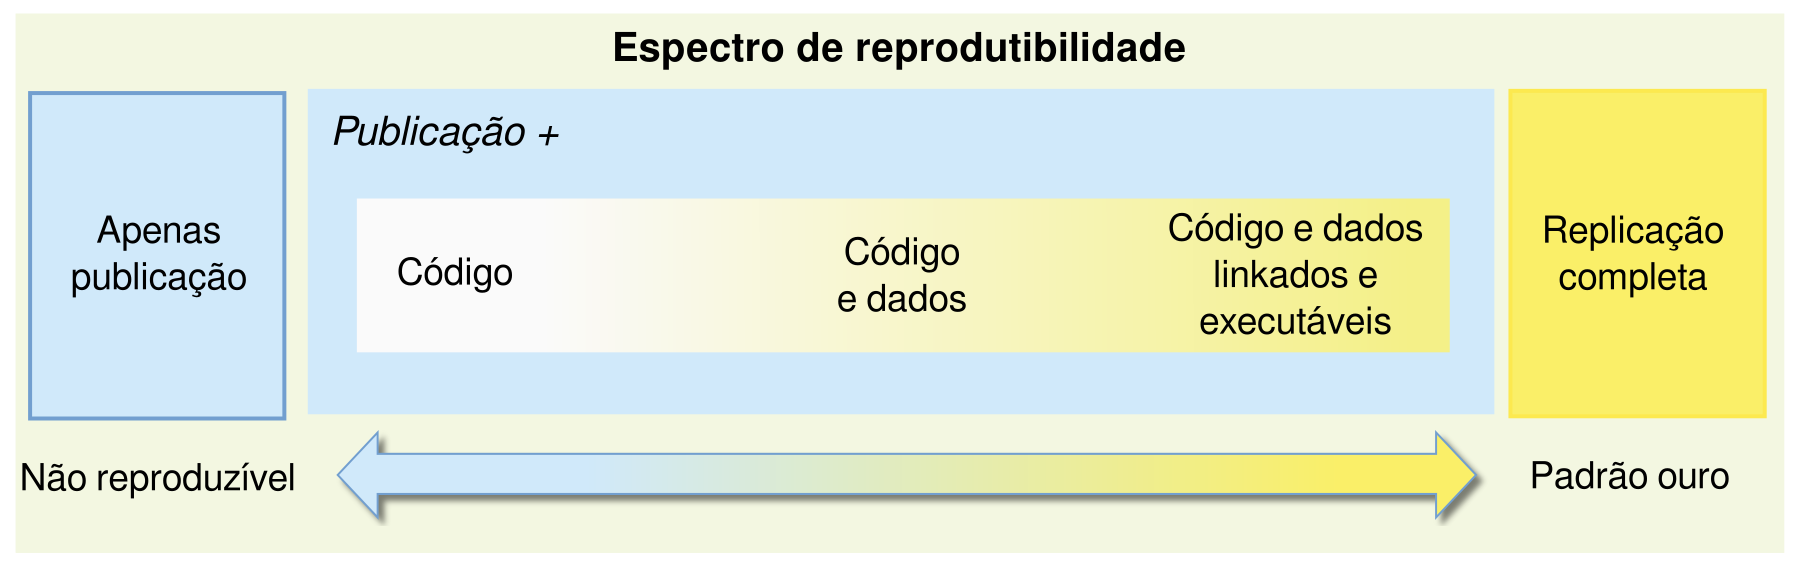
\includegraphics[scale=0.35]{imagens/reproducibility-spectrum-ptbr.png}
  \caption{Espectro de reprodutibilidade \cite{Peng2011}}
  \label{reproducibility-spectrum}
\end{figure}

Apesar das pesquisas reproduzíveis ({\it RR - Reproducible Research}) não
resolverem todos os problemas de validade experimental dos estudos em
engenharia de software, elas ao menos garantem que dados e métodos de análise
estejam disponíveis para inspeção e que os resultados possam ser derivados,
facilitando revisão logo que a publicação acontece. Além disso, é um recurso
valoroso para pesquisadores iniciantes, pesquisas reproduzíveis melhoram o
impacto do próprio estudo, por exemplo, artigos de computação que não
disponibilizam pubicamente dados e códigos possuem menos chances de serem
citados \cite{madeyski2017would}.

A disponibilidade dos softwares científicos tem sido enfatizada também em
discussões sobre sustentabilidade de software, um conceito que diz respeito
à longevidade dos sistemas de software.

%% O surgimento do conteito de engenharia de software baseada em envidências (EBSE
%% - {\it Evidence-Based Software Engineering }) surgiu em um trabalho seminal
%% apresentado em 2004 na {\it International Conference on Software Engineering
%% (ICSE)} e suas ideias e ferramentas, especialmente a revisão sistemática, tem
%% evoluído e amadurecido ao longo do tempo, e tem ajudado a caracterizar e
%% consolidar nosso conhecimento sobre muitos aspectos da pesquisa e práticas da
%% engenharia de software.
%% 
%% Em engenharia de software o termo {\it literatura} foi adicionado formando
%% revisão sistemática de literatura, isto foi feito para evitar confusão com
%% práticas de inspeção de código (comumente definido com o termo revisão) existentes
%% na área.
%% 
%% O objetivo de uma revisão sistemática é buscar e identificar todo material relevante
%% relacionado a um certo tópico (a natureza deste material é determinada pelas
%% questões de pesquisa e a natureza dos participantes intererssados na pesquisa).
%% 
%% Um fator em favor da aceitação dos conceitos da EBSE tem sido a crescente
%% reconhecimento que os resultados de estudos empíricos individuais são frequentemente
%% inconclusivos, e estes tipo de estudos são difícels de replicar com sucesso
%% \cite{sjoberg2005survey}.
%% 
%% Ainda existem poucos estudos replicados \cite{kitchenham2015evidence}.

\section{Sustentabilidade de software} \label{sustentabilidade}

% Software Sustainability: The Modern Tower of Babel

O {\it Dagstuhl Perspective Workshop} é um evento organizado por e para um
pequeno grupo de pesquisadores sêniores de renome internacional, realizado
anualmente na universidade de Dagstuhl\footnote{\url{http://www.dagstuhl.de}}
com o objetivo de refletir sobre o atual estado da ciência da computação.

Através de uma discussão intensiva com foco estratégico o workshop explora
tópicos novos e emergentes da ciência da computação produzindo manifestos que
capturam tendências e desenvolvimentos relacionados aos tópicos explorados.

Realizado desde 2011 o workshop tem explorado diversos tópicos da ciência da
computação, como computação e paleografia, tecnologia da informação como ponte
entre biologia e medicina, métodos de aprendizado de máquina para segurança de
computadores, análise de performance e visualização, entre outros tópicos. Em
sua mais recente edição, o {\it Dagstuhl Perspectives Workshop on ``Engineering
Academic Software''} \cite{allen2017engineering} examinou o estado atual dos
softwares científicos, identificou problemas comuns em seu desenvolvimento,
reconhecimento e sustentabilidade.

Uma das contribuições chave deste workshop é um manifesto contendo um roteiro
para o futuro da engenharia de software profissional e acadêmica, com foco em
instrumentos de suporte para pesquisas em software científico. O manifesto é
expresso em termos de ações ``promessas'' destinado a usuários e
desenvolvedores de softwares científicos, com passos concretos para melhorar o
ambiente em que os softwares são produzidos.

Os compromissos expressados neste manifesto são agrupados em três conceitos gerais:
(i) garantir que softwares científicos sejam {\it citados} apropriadamente;
(ii) promover a {\it carreira} do engenheiro de software desenvolvedor de software científico; e
(iii) medir a qualidade e sustentabilidade do software científico durante e após o seu {\it desenvolvimento}.

No terceiro compromisso, relacionado ao conceito {\it desenvolvimento}, o Dagstuhl Manifesto enfatiza a necessidade de medir a
qualidade e a sustentabilidade dos softwares científicos, e define
sustentabilidade de software como capacidade de perdurar, software sustentável
é aquele que continua a estar disponível no futuro, em novas plataformas e se
atende às novas necessidades \cite{allen2017engineering}.

% campos da engenharia de software, e apesar dos inúmeros entendimentos sobre o
% conceito \cite{venters2014software}, 

Essa definição de sustentabilidade de software é encontrada em mais detalhes no
{\it Karlskrona Manifesto} \cite{becker2014karlskrona}, um documento que alerta
sobre os impactos que os sistemas e a tecnologia da informação causam no futuro
do planeta, convida praticantes e pesquisadores de software a refletir sobre
o tema sustentabilidade na área da ciência da computação.

Sustentabilidade é um conceito guarda chuva composto de múltiplas dimensões, em
sua dimensão técnica, chamada sustentabilidade técnica, temos a preocupação com
a longevidade da informação, dos sistemas, e infraestrutura, e sua adequada
evolução frente as condições do ambiente em constante mudança. Software ocupa
um papel central nessa discussão, ele pode levar a crescentes consumo de
recurso, crescimento da desigualdade social, e influenciar no ganho ou perda de
auto-estima individual.

Se sustentabilidade não for levada em consideração em projetos de software, não
importa qual o domínio ou qual o propósito do software, perde-se a oportunidade
de causar mudanças positivas no planeta e na sociedade.

%Pesquisadores de
%software podem contribuir identificando questões de pesquisa em seu campo para
%ajudar a melhor entender sustentabilidade em projetos de software, Discutir com
%seus pares e pensar sobre como sustentabilidade impacta sua área de pesquisa.
%
%Assim, surge um conjunto de ações que podem ser tomadas pelos diferentes atores
%em direção à garantir sustentabilidade nos projetos de software, ações para
%praticantes de software, pesquisadores, associações profissionais, educadores,
%cientes e usuários.
% 
% 
% Em resumo os dois manifestos, Dagstuhl e Karlskrona, exprimem o conceito de
% sustentabilidade necessários para este estudo, mas é importante citar que
% algumas iniciativas e outros manifestos também estão preocupados com questões
% similares, dentre os quais podemos destacar:
% 
%A ciência aberta e comunidades de pesquisa em software tem sido bastante ativas
%em criar manifestos visando chamadas para ação. Estes manifestos chamam para melhorar
%os softwares e os metadados de bibliografia para citação persistente destes softwares.
%Outros tópicos endereçados nestes manifestos incluem ênfase no acesso ao código fonte.
%
%Agências de financiamento como o {\it US National Science Foundation} estão começando
%a reconhecer produtos de pesquisa como software assim como fazem com as publicações.
%Isto reconhece as contribuições ao softwares assim como primeiro produto de pesquisa.
%
%O {\it Journal of the American Statistical Association (JASA)} irá agora insistir na
%disponibilidade do código e dados durante a revisão dos manuscritos \cite{baker2016scientists}.
%% 
%% \begin{itemize}
%% 
%%   \item Science Code Manifesto \cite{barnes2013science}
%% 
%%     Foco em código fonte escrito especificamente para processar dados de
%%     publicações, afirma que ``todo código fonte escrito especificamente para
%%     processar dados de uma publicação deve estar disponível para os revisores e
%%     leitores do paper''.
%% 
%%   \item FORCE11 Software Citation principles \cite{smith2016software}\footnote{\url{https://www.force11.org/software-citation-principles}}
%% 
%%     Enfatiza persistencia e claridade e diz que ``Software deve ser considerado
%%     um produto legítimo de pesquisas e devem ser possível de serem citados''.
%% 
%%   \item Open Access Pledge \cite{holcombe2011openaccess}\footnote{\url{http://www.openaccesspledge.com}}
%% 
%%     Concentra-se em publicar softwares e papers em locais de {\it open access}.
%% 
%%   \item Open Science Peer Review Oath\footnote{\url{https://f1000research.com/articles/3-271/v2}}
%% 
%%     Concentra-se em potencializar os revisores para exigir acesso aberto aos
%%     softwares, práticas reprodutíveis e revisões transparentes.
%% 
%%   \item UK RSE \cite{ukrse2013}\footnote{\url{http://rse.ac.uk/who}}
%% 
%%     Conscientização sobre a importância e o papel do {\it Research Software
%%     Engineer} através de comunicação e suporta institucional.
%% 
%%   \item Reproducibility manifesto \cite{Barba2012}\footnote{\url{http://lorenabarba.com/gallery/reproducibility-pi-manifesto}}
%% 
%%     Inclui termos para fazer softwares reusáveis por outros. Foco em
%%     reprodutibilidade, deixando sustentabilidade de software fora de questão.
%% 
%%   \item The GeoScience paper of the future initiative \cite{OntoSoft2016}\footnote{\url{http://www.scientificpaperofthefuture.org/gpf/what-is-a-gpf}}
%% 
%%     Possui um conjunto de requerimentos para softwares serem incluidos em
%%     papers.  Focando mais no paper em sí do que no software.
%% 
%%   \item FAIR principles \cite{wilkinson2016fair}\footnote{\url{https://www.nature.com/articles/sdata201618}}
%% 
%%     Foco em dados de pesquisa. O objetivo é fazer eles serem encontráveis,
%%     acessíveis, interoperável e reusável. Estes princípios podem ser
%%     generalizados para aplicar aos softwares.
%% 
%% \end{itemize}

\section{Análise estática de código fonte} \label{analise-estatica}

A análise estática de código fonte é o primeiro passo para coletar informações
necessárias em diversas atividades de verificação, medição e melhoria da
qualidade de produtos de software \cite{Cruz2009, Kirkov2010}. Ela é
realizada com base no código fonte de um programa ou sistema de software, e a
partir daí descobre problemas e propriedades de sua qualidade estrutural
\cite{Chess2007}.

Ferramentas de análise estática estão disponíveis há décadas, em especial,
para programadores. A ferramenta Lint \cite{Johnson1978}, considerada a
primeira ferramenta de análise estática \cite{Gosain2015}, foi criada para
examinar programas escritos em linguagem C e aplicar regras de tipagem mais
estritas do que as regras dos próprios compiladores da linguagem.

%Neste trabalho o nosso interesse reside em compreender características de
%qualidade interna de ferramentas deste domínio de aplicação, do ponto
%de vista de desenvolvedores interessados em manter e evoluir tais ferramentas
%melhorando seus atributos de qualidade interna.
%
%A seção \ref{analise-estatica} apresenta uma definição geral da análise
%estática de código fonte, suas aplicações, sua anatomia, seus formatos de
%representação intermediária e técnicas mais comuns. 

Análise estática de código fonte tem como objetivo prover
informações acerca de um programa a partir do seu código fonte sem
necessidade de execução, e sem requerer qualquer outro artefato do programa
além do próprio código.

É um ramo que possui muitas das suas abordagens em comum com os estudos da
área de análise de programas ({\it program analysis}), especialmente na área de
compiladores, onde atua especialmente nas primeiras etapas do processo de compilação.

A análise estática de código fonte é considerada uma atividade meio com
objetivo de suportar uma variedade de tarefas comuns da engenharia de
software; muitas dessas tarefas são substancialmente úteis em atividades de
manutenção. \citeonline{Binkley2007} define uma lista dessas
atividades, incluindo:

\begin{multicols}{2}
  \begin{itemize}
    \item Análise de performance
    \item Compreensão de programas
    \item Desenvolvimento baseado em modelos
    \item Detecção de clones
    \item Evolução de software
    \item Garantia de qualidade
    \item Localizaçao de falhas
    \item Manutenção de software
    \item Recuperação arquitetural
    \item Testes
  \end{itemize}
\end{multicols}

Seja em qual atividade for, a análise estática possui importância,
pois ao ser capaz de extrair informações diretamente do
código fonte de um programa, pode auxiliar a responder perguntas necessárias
para as diversas atividades de desenvolvimento e evolução de software. Essa
importância se torna ainda mais aparente diante da ``lei'' da tendência para
execução \cite{Harman2010} que indica que todos os tipos de notação tem a
tendência de se tornar executáveis.

\subsection{Usos da análise estática de código fonte} \label{usos}

A análise de programas trata, de modo geral, da descoberta de problemas e
fatos sobre programas, ela pode ser realizada sem a necessidade de executar o
programa (análise estática) ou com informações provenientes de sua execução
(análise dinâmica).

A ideia de que programas de computador podem ser utilizados para analisar
código fonte de outros programas tem uma história de mais de 40 anos.  O
programa PFORT \cite{Ryder1974} foi projetado para localizar potenciais
problemas na portabilidade de código Fortran; em função da diversidade de
dialetos de Fortran, uma compilação sem erros não indicava que o programa
estava correto segundo os padrões da linguagem \cite{Wichmann1995}.

Desde então, ferramentas de análise estática de código fonte têm surgido para
os mais diversos fins -- muitas delas a partir das pesquisas e
desenvolvimentos da área de compiladores.  O {\it parser} utilizado nessas
ferramentas têm funcionalidades análogas aos analisadores usados em
compiladores \cite{Anderson2008}.

O uso de tais ferramentas tem se
tornado mais comum no ciclo de desenvolvimento de
software, sendo aplicadas em uma infinidade de atividades distintas visto que o
campo de aplicação destas ferramentas é bastante variado, cobrindo diferentes
objetivos. De acordo com \citeonline{Chess2007}, as atividades em que análise
estática de código fonte é empregada, destacam-se:

\begin{description}

  \item \textit{Verificação de tipos}. 
    A forma mais amplamente utilizada de análise estática, e uma das quais os
    programadores estão mais familiarizados, é a checagem de tipo.
    Previne que acidentalmente atribuam valores de forma incorreta a
    variáveis. Ainda, ao capturar erros em tempo de compilação, esta checagem
    de tipo previne erros em tempo de execução.

  \item \textit{Verificação de estilo}. 
    Os verificadores de estilo são um tipo de análise estática que aplicam regras
    de forma mais superficial do que os verificadores de tipo. São regras
    relacionadas a espaços em branco, nomes, funções depreciadas, comentários,
    estrutura do programa, entre outros. Os erros reportados por verificadores de
    estilo são aqueles que afetam a leitura e a manutenabilidade do
    código fonte, não indicando potenciais erros em tempo de execução como
    fariam os verificadores de tipo.

  \item \textit{Compreensão de programas}. 
    Ferramentas de compreensão de programa ajudam programadores a terem uma visão
    clara frente a grandes programas de computador, ou seja, programas com
    alto volume de código fonte. Ambientes de desenvolvimento integrados (IDE)
    geralmente incluem funcionalidade de compreensão, por exemplo, ``encontrar
    todos os usos de um certo método'' ou ``encontrar a declaração de uma
    variável global''. Análises mais avançadas chegam a incluir, por exemplo,
    refatoração automática. Estas ferramentas de compreensão também são úteis
    para programadores interessados em entender código fonte escrito por
    outros programadores.

  \item \textit{Verificação de programas}.
    Ferramentas de verificação de programa aceitam como entrada uma especificação
    e um conjunto de código fonte e tenta provar que o código está deacordo
    com a especificação. Quando a especificação é uma descrição completa de
    todo o programa, a ferramenta de verificação poderá realizar uma checagem
    de equivalência para garantir que o código fonte e a especificação
    combinam de forma exata. Programadores raramente têm acesso a uma
    especificação detalhada suficientemente para ser usada numa checagem de
    equivalência, o trabalho de criar esta especificação pode ser maior do que
    o trabalho de escrever o próprio código fonte do programa, desta forma
    este tipo de verificação formal raramente acontece.

  \item \textit{Localização de bugs}. 
    Um localizador de bugs está
    preocupado em apontar locais onde o programa, possivelmente, irá se
    comportar de forma inesperada. A maioria das ferramentas de localização de
    bugs são fáceis de usar porque costumam vir com um conjunto de regras
    ({\it bug idioms}) para descrição de padrões de código que indicam bugs.
    Algumas destas ferramentas costumam usar os mesmos algoritmos utilizados
    por ferramentas de verificação de propriedade.

  \item \textit{Avaliação de segurança}. 
    Ferramentas de análise estática para segurança usam as mesmas técnicas
    encontradas nas outras ferramentas, mas por ter um propósito diferente,
    identificar problemas de segurança, aplicam estas técnicas de forma diferente.
    As primeiras ferramentas de segurança (ITS4, RATS, Flawfinder) eram pouco mais
    do que um {\it ``grep''} melhorado; na maior parte, elas escaneavam o código
    procurando por funções como por exemplo {\it ``strcpy()''} que são
    facilmente usadas de forma inadequada e devem ser inspecionadas
    manualmente no processo de revisão de código fonte.

\end{description}

\subsection{Anatomia da análise de código fonte} \label{anatomia}

Ferramentas de análise estática de código fonte estão organizadas em partes ou
componentes, responsáveis por implementar três funções básicas: a) extração de dados, b) geração de representação
intermediária, e c) análise \cite{Cruz2009, Binkley2007}.

\begin{description}

  \item \textit{Extração de dados}.
    O processo de recuperar dados para futuro processamento ou armazenamento é
    chamado de extração de dados. 

    O primeiro componente da análise de código fonte é a extração de dados,
    responsável por ler o código fonte do programa e gerar uma ou mais
    representações intermediárias. Em essência, este componente converte a sintaxe
    de um programa em uma outra sintaxe abstrata e mais adequada para análise
    posterior.

  \item \textit{Representação intermediária}.
    Exportar os dados extraídos para uma representação intermediária é uma
    estratégia comum para facilitar análise e transformação de dados e
    possivelmente adição de metadados.

    Os dados obtidos na extração precisam ser representados em um formato mais
    abstrato. Esta é a responsabilidade do segundo componente da análise de
    código fonte: armazenar os dados coletados usando uma representação
    intermediária em formato mais adequado para análise automática, abstraindo
    aspectos particulares do programa e da linguagem de programação.

    Alguns tipos de representação intermediária têm sua origem na área de
    compiladores, entre os formatos mais comuns, destacam-se:

    \begin{multicols}{2}
      \begin{itemize}
        \item Árvore sintática abstrata
        \item Grafo de fluxo de controle
        \item Árvore sintática abstrata decorada
        \item Grafo de dependência de módulos
        \item Atribuição estática única
        \item Grafo de dependência de valores
      \end{itemize}
    \end{multicols}

    Estas representações podem ser utilizadas tanto na análise estática quanto
    na análise dinâmica. O uso de um ou outro formato depende do tipo de
    análise e seu propósito. Pode-se combinar diferentes tipos no sentido de
    enriquecer e estruturar a informação extraída.

  \item \textit{Análise}.
    Este componente é responsável por realizar inferências a partir dos dados
    representados internamente. O processo requer que as informações
    armazenadas estejam interconectadas e também interrelacionadas com
    conhecimento anterior. Esta análise pode gerar conhecimento quantitativo
    ou qualitativo, como, por exemplo, métricas de software ou mineração de
    dados, respectivamente. Técnicas de visualização podem ser usadas para
    apoiar este processo.

    Diversas técnicas foram desenvolvidas ao longo do tempo para realizar
    análise, algumas delas são brevemente descritas na seção \ref{tecnicas}.

\end{description}

\subsection{Formatos de representação intermediária} \label{formatos}

Essencialmente, um formato de representação intermediária é uma abstração precisa
das propriedades de um programa representado em um domínio menor. Os
compiladores normalmente constroem esta representação a fim de possuir um
modelo do programa sendo compilado, é comum que compiladores utilizem diversos
formatos durante o curso da compilação.

Em ferramentas de análise estática estes formatos são utilizados durante a
fase de análise para cumprir diversos objetivos, como por exemplo, calcular
métricas de código fonte. A métrica de complexidade ciclomática de McCabe
\cite{McCabe1976}, por exemplo, é definida com base no grafo de fluxo de controle ({\it Control Flow Graph - CFG}) do
programa com o seguinte cálculo $CC = e - n + 2p$. Onde: {\bf e} é o número de
arestas; {\bf n} é o número de nós; e {\bf p} é o número de componentes
fortemente conectados no grafo.

Assim, percebe-se que cada formato de representação intermediária pode ter fins
e objetivos bastante distintos, dentre os formatos mais comuns podemos destacar
\cite{Nielson2015, Stanier2013, Cruz2009, Ramalho1996}:

\begin{description}

  \item \textit{Árvore sintática abstrata}.
    A árvore sintática abstrata (AST - {\it Abstract Syntax Tree}) representa um
    programa tratando os elementos do código fonte como operadores e
    operandos organizados em nós numa árvore, este formato de representação é
    muito popular em tradutores {\it
    source-to-source}\footnote{http://en.wikipedia.org/wiki/Source-to-source\_compiler}.

  \item \textit{Grafo de fluxo de controle}.
    O grafo de fluxo de controle (CFG - {\it Control Flow Graph} ou {\it Call Graph}) é um grafo direcionado
    representando a estrutura de controle de um programa e sua sequência de
    instruções, onde as arestas mostram os possíveis caminhos de execução. Este
    formato é amplamente utilizado em métodos formais para otimização de
    código fonte.

  \item \textit{Grafo de fluxo de dados}.
    O grafo de fluxo de dados (DFG - {\it Data Flow Graph}) é também um grafo
    direcionado onde as arestas representam o fluxo de dados entre as
    operações do programa, este formato pode ser visto como um companheiro do
    grafo de fluxo de controle (CFG) e pode ser gerado ao longo de uma mesma
    análise.

  \item \textit{Árvore sintática abstrata decorada}.
    Árvore sintática abstrata decorada (DAST - {\it Decorated Abstract Syntax Tree}) é
    uma árvore sintática abstrata (AST) melhorada através de um processo de
    definiçao de atributos para os símbolos do programa de forma declarativa
    com uso de uma Gramática de
    Atributos\footnote{https://en.wikipedia.org/wiki/Attribute\_grammar}.

  \item \textit{Grafo de dependência de módulos}.
    O grafo de dependência de módulos (MDG - {\it Module Dependence Graph}) é um grafo
    onde os módulos são representados como nós e as arestas representam as
    relacões entre eles, indicando dependência entre os mesmos.

  \item \textit{Atribuição estática única}.
    Atribuição estática única (SSA - {\it Static Single Assignment}) pode ser vista
    como uma variação ou uma propriedade de outros formatos de representação
    intermediária, é um método que faz cada variável ser atribuída apenas uma única
    vez, facilitando a descoberta de informaçoes sobre os dados representados.

  \item \textit{Grafo de dependência de valores}.
    O grafo de dependência de valores (VDG - {\it Value Dependence Graph}) é uma
    variação que melhora (ao menos para algumas análises) os resultados
    obtidos a partir da atribuição estática única (SSA). Ele representa tanto
    o fluxo de controle quanto o fluxo de dados e assim simplifica a análise.

\end{description}

\subsection{Técnicas de análise} \label{tecnicas}

Inúmeras técnicas e métodos distintos podem ser utilizados pelas ferramentas
de análise estática, seja com o objetivo de verificação de tipos, localização
de bugs, compreensão de programas, avaliação de segurança, ou outra finalidade
qualquer. Segundo \citeonline{German2003, Li2010, Hofer2010} as técnicas e
métodos mais comumente encontrados nas ferramentas atuais são:

\begin{description}

  \item \textit{Análise léxica}.
    A análise léxica é responsável por quebrar o programa em pequenos fragmentos
    (ou {\it tokens}) e verificar se estes fragmentos são palavras válidas
    para uma dada linguagem. A análise léxica não leva em consideração a
    sintaxe do programa, sua semântica ou a interação entre módulos.

  \item \textit{Combinação de padrões de texto}.
    A combinação de padrões de texto ({\it Text-based Pattern Matching}) é a
    maneira mais simples e rápida de procurar vulnerabilidades num código
    fonte.

  \item \textit{Inferência de tipos}.
    A inferência de tipos ({\it Type inference}) refere-se a identificar o
    tipo de variáveis e funções e avaliar se o acesso a elas está em
    conformidade com as regras da linguagem. Linguagens de programação com
    sistema de tipagem incluem mecanismos deste tipo de análise.

  \item \textit{Análise de fluxo de dados}.
    A análise de fluxo de dados ({\it Data flow analysis}) resume-se a coletar
    informação semântica do código fonte do programa, e com métodos algébricos
    deduzir a definição e uso das variáveis em tempo de compilação. O objetivo
    é mostrar que nenhum caminho de execução do programa acessa uma variável
    sem definição ou atribuição prévia.

  \item \textit{Verificação de regra}.
    A verificação de regra ({\it Rule checking}) consiste em checar a segurança
    do programa através de um conjunto de regras pré-estabelecidas.

  \item \textit{Análise de restrição}.
    A análise de restrição ({\it Constraint analysis}) consiste em gerar
    e resolver restrições no processo de análise de um programa.

  \item \textit{Comparação caminho}.
    Comparação caminho ({\it Patch comparison}) inclui comparação de caminho de
    código fonte e de código-binário e é usada principalmente para encontrar
    brechas de vulnerabilidade já ``conhecidas'' e previamente divulgadas por
    fornecedores e praticantes da indústria de software.

  \item \textit{Execução simbólica}.
    A execução simbólica ({\it Symbolic execution}) é usada para representar
    as entradas de um programa através do uso de valores simbólicos ao invés
    de dados reais, produz expressões algébricas sobre a entrada dos símbolos
    do programa durante o processo de implementação e pode detectar
    possibilidade de erros.

  \item \textit{Interpretação abstrata}.
    Interpretação abstrata ({\it Abstract interpretation}) é uma descrição
    formal da análise do programa. Pelo fato de apenas controlar atributos de
    programa de preocupaçao dos usuários, a interpretação da análise semântica
    é similar ao seu significado semântico real.

  \item \textit{Prova de teoremas}.
    Prova de teoremas ({\it Theorem proving}) é baseada na análise semântica do
    programa. Converte o programa em fórmulas lógicas e então tenta provar que
    o programa é um teorema válido usando regras e axiomas.

  \item \textit{Verificação de modelo}.
    O processo de verificação de modelos ({\it Model checking}) primeiro constrói
    um modelo formal do programa tal como uma máquina de estados ou um grafo
    direcionado, então examina e compara o modelo para verificar se o sistema
    cumpre as características pré-definidas. Esta técnica requer a definição e
    descrição das propriedades que devem ser verificados por um pedaço de
    software.

  \item \textit{Verificação formal}.
    Verificação formal ({\it Formal Checking} ou {\it Compliance Analysis}) é o
    processo de provar de forma automatizada que o código do programa está
    correto em relação a uma especificação formal dos seus requisitos.

  \item \textit{Análise de fluxo da informação}.
    Análise de fluxo da informação ({\it Information Flow Analysis}) identifica
    como a execução de uma unidade de código cria dependência entre entradas e
    saídas.

  \item \textit{Verificação de sintaxe}.
    Verificação de sintaxe ({\it Syntax Checks}) tem o objetivo de encontrar
    violação de regras tais como expressões mal-formadas ou fora do padrão.

  \item \textit{Verificação de intervalo}.
    A análise de verificação de intervalo ({\it Range Checking}) tem o objetivo
    de verificar que os valores dos dados permanecem dentro de intervalos
    especificados, bem como manter a precisão especificada.

\end{description}

Diante a variedade e a constante evolução da área de análise estática
\citeonline{Novak2010} fez um estudo propondo uma taxonomia e um conjunto de
dimensões para caracterização de ferramentas de análise estática, mais detalhes
sobre essas dimensões e categorias serão exploradas no Capítulo
\ref{caracterizacao-ferramentas}, no qual apresentaremos uma caracterização de
softwares científicos estudados neste trabalho.

\section{Complexidade estrutural} \label{complexidade}

%% Métricas de software podem ser classificadas em métricas de processo, métricas
%% de projeto e métricas de produto.
%% 
%% Métricas de processo medem atributos relacionados ao ciclo de desenvolvimento
%% e manutenção de software. Métricas de projeto indicam se a execução do
%% processo está progredindo conforme planejado (por exemplo, relação entre o
%% tamanho do software entregue e o esforço total dispendido em seu
%% desenvolvimento).
%% 
%% Métricas de produto medem atributos de produtos e artefatos, como documentos,
%% diagramas, código fonte e arquivos binários. Neste trabalho,
%% apenas métricas de produto serão utilizadas.
%% 
%% Métricas de produto podem ser classificadas em internas (medem propriedades
%% visíveis apenas aos desenvolvedores) ou externas (medem propriedades visíveis
%% aos usuários) \cite{Mohamed1994}.
%% 
%% Neste trabalho, são utilizadas métricas de produto e, especificamente,
%% métricas de código fonte, que cobrem aspectos de tamanho, complexidade e
%% qualidade que podem ser medidos a partir do código fonte de um software.
%% 
%% Métricas de software tem um escopo bastante abrangente, e o termo está
%% associado com muitas atividades da engenharia de software: Medidade e modelos
%% para estimativa de custo e esforço, Coleção de dados, Modelos e medidas de
%% qualidade, Modelos de confiabilidade, Métricas de segurança, Métricas
%% estruturais e de complexidade, Avaliação de maturidade de capacidade,
%% Gerenciamento através de métricas, Avaliação de métodos e ferramentas.
%% 
%% \subsection{Métricas de código fonte} \label{metricas-de-codigo}
%% 
%% As propriedades visíveis aos desenvolvedores podem ser medidas através de
%% métricas de código fonte. A observação e o monitoramento de seus valores podem
%% indicar aspectos relevantes à manutenibilidade de um programa. Dentre as
%% inúmeras métricas de código fonte nosso interesse está em métricas que indicam
%% características relevantes à modularidade de um produto de software,
%% complexidade estrutural e custo de mudança.

%Structural and Complexity Metrics
%Desirable quality attributes like reliability and maintainability cannot be
%measured until some operational version of the code is available. Yet, we
%wish to be able to predict which parts of the software system are likely to be
%less reliable, more difficult to test, or require more maintenance than oth-
%ers, even before the system is complete. As a result, we measure structural
%attributes of representations of the software that are available in advance
%of (or without the need for) execution; then, we try to establish empiri-
%cally predictive theories to support quality assurance, quality control, and
%quality prediction. These representations include control flow graphs that
%usually model code and various unified modeling language (UML) dia-
%grams that model software designs and requirements. Structural metrics
%can involve the arrangement of program modules, for example, the use
%and properties of design patterns. These models and related metrics are
%described in Chapter 9.

Do ponto de vista de métricas, neste trabalho, estamos interessados, de fato, na métrica
de complexidade estrutural SC ({\it Structural Complexity}), uma medida da
complexidade de projetos de sistema de software proposta por
\citeonline{Darcy2005} como indicador da complexidade dos sistemas de software
em relação à sua estrutura interna e ao relacionamento entre os seus
componentes.

Complexidade é um tema bastante amplo, e para compreender onde os
sistemas de softwares se encaixam neste contexto precisamos definir brevemente
o que vem a ser sistemas complexos.

Sistemas complexos são sistemas no qual grandes redes de componentes sem
controle central dão origem a um comportamento
coletivo complexo, com processamento sofisticado de informação, e adaptação
através de aprendizado ou evolução \cite{Mitchell2009}. As seguintes
características são comuns a todos os sistemas complexos:

\begin{description}

  \item[Comportamento coletivo complexo.] Apesar de serem compostos por
  elementos bastante simples individualmente, sistemas complexos podem exibir
  comportamentos coletivos bastante sofisticados.

  \item[Troca de sinais e processamento de informação.] Em cada um destes
  sistemas, seus componentes individuais consomem e produzem informação entre
  si. Parte do comportamento do sistema envolve transformação dessa informação.

  \item[Adaptação.] Sistemas complexos adaptam-se a novas situações de forma a
  aumentar suas chances de sobrevivência diante de novas condições em seu
  ambiente.

\end{description}

Os sistemas complexos podem ser classificados como naturais ou artificiais, os
sistemas naturais são aqueles cuja constituição não tem participação humana, ao
contrário dos sistemas artificiais que são projetados por humanos, com
objetivos e funções previamente definidos \cite{Simon1996}. Neste sentido,
sistemas de software podem ser caracterizados como sistemas complexos
artificiais, pois exibem comportamento coletivo complexo, realizam trocas de
sinais e processamento de informação e passam por adaptação para se adequar a
mudanças em seu ambiente.

Sistemas de software são compostos por componentes, em geral, chamados de
módulos, que possuem tanto estado quanto comportamento próprios,
módulos individuais de um sistema de software são simples quando comparados com
o sistema como um todo. Módulos produzem informação para outros módulos
através de parâmetros em chamadas de sub-rotinas e consomem informação através
dos valores de retornos destas chamadas. O fluxo contínuo de novos requisitos e
de mudanças no ambiente operacional de sistemas de software força-os a se
manter em constante evolução em busca de “sobrevivência”.

Esta medida é, possivelmente, um indicativo de problemas na manutenibilidade de
sistemas de software, em especial sobre o esforço necessário para atividades de
manutenção \cite{Terceiro2012}. Ela está relacionada a como os módulos de um
programa estão organizados bem como à estrutura interna de cada módulo. Esta
métrica pode dar indícios importantes sobre características arquiteturais de um
programa de software e pode explicar seus atributos de qualidade interna.

%Modularity
%Modularity describes the logical partitioning of software into several parts, components, and modules.
%Software will be easy to understand and change when composed of independent modules.
%“A Software Maintainability Evaluation Methodology”, 1981
%\cite{kumar2012survey}

%Faz um experimento usando CBO LCOM e outras metricas como preditor de manutenabilidade...
%\cite{Dagpinar2003}

%A complexidade de um sistema de software pode ser de três tipos: a complexidade
%do problema, a complexidade procedural, e a complexidade do projeto do sistema.
%Esta última é o foco deste trabalho.
%A complexidade do problema está relacionada ao domínio do problema.
%A complexidade procedural está relacionada à estrutura lógica da programa, em es-
%pecial do seu comprimento, em termos de número de tokens, linhas de código fonte, ou
%estruturas de controle. Este último tipo é o que iremos estudar neste trabalho.
%
%Os sistemas complexos podem naturais ou artificiais, uma colônia de formigas
%por exemplo pode ser caracterizado como um sistema complexo natural, onde
%individualmente cada formiga se apresenta como criatura relativamente simples,
%com instintos básicos como procurar alimento, responder a estímulos químicos
%vindos de outras formigas, combater intrusos, etc. No entanto, quando
%observadas coletivamente em uma colônia, as formigas aparentam ser muito mais
%sofisticadas. Elas são capazes de se organizar em diferentes atividades, criar
%estruturas complexas dentro de seu formigueiro, e de encontrar o caminho mais
%curto para uma fonte de alimento.
%
%Os sistemas naturais são aqueles cuja constituição não tem participação humana.
%Sistemas artificiais são projetados por humanos, com objetivos e funções
%definidos.  Sistemas artificiais podem ou não serem projetados à imagem de um
%sistema natural, e durante a sua concepção eles são discutidos em termos tanto
%de suas características (o que eles são) como de necessidades que eles devem
%satisfazer (o que eles deveriam ser) \cite{Simon1996}.
%
%É importante ressaltar que esta caracterização de sistemas de software como
%sistemas complexos diz respeito à estrutura interna dos sistemas, ou seja, aos
%componentes que o constituem e ao relacionamento entre estes componentes. Não
%foram considerados outros aspectos importantes de sistemas complexos, como por
%exemplo o seu relacionamento com o ambiente externo.
%
%como uma combinação das métricas de acoplamento (CBO) e coesão (LCOM4), 
%
%Sistemas de software, no entanto, se
%diferenciam dos sistemas complexos naturais pelo fato de serem projetados;
%consequentemente, o seu processo evolucionário não é intrinsecamente parte do
%seu comportamento, mas fruto da ação consciente de seus desenvolvedores.
%
%\cite{Tegarden1995}
%
%"The implication of this result is that, when
%designing, implementing, and maintaining software to control complexity, both coupling and cohesion should be considered jointly,
%instead of independently" Darcy 2005
%
%Many studies have demonstrated a significant correlation between
%LOC and the cyclomatic number. The researchers usually suggest that
%this correlation proves that cyclomatic number increases with size; that
%is, larger code is more complex code. However, careful interpretation of
%the measures and their association reveals only that the number of deci-
%sions increases with code length, a far less profound conclusion. The cyclo-
%matic number may be just another size measure. Chapter 9 contains more
%detailed discussion of validation for the McCabe measures.
%
%{\bf SC} {\it Structural Complexity (Complexidade estrutural)}: mede a
%complexidade do software \cite{Darcy2005} combinando os valores de CBO e LCOM4.

\citeonline{Darcy2005} definem complexidade estrutural como uma combinação de
acoplamento e coesão. Estes são dois conceitos complementares: enquanto o
acoplamento reflete o relacionamento entre módulos, a coesão nos fornece uma
visão da organização dos componentes internos de um módulo e seus
relacionamentos.

Uma formalização da métrica proposta por \citeonline{Darcy2005} pode ser
expressa da seguinte maneira, para um projeto $p$ e seu conjunto de módulos
$M(p)$, a complexidade estrutural $SC(p)$ de $p$ é:

\begin{equation}
SC(p) = \frac
{ \displaystyle \sum_{m \in M(p)} CBO(m) \times LCOM4(m) }
{ |M(p)| }
\end{equation}

Esta medida de complexidade estrutural é portanto a complexidade
estrutural média entre todos os módulos do sistema.

\begin{itemize}

  \item {\bf CBO} {\it Coupling Between Objects (Acoplamento entre objetos)}:
    mede o acoplamento entre objetos do software \cite{Chidamber1994}
    calculando em nível de classe o número total de acessos à outras classes do
    mesmo sistema, é comum ser também chamada de Fan-out da classe. CBO é então
    definida pela seguinte fórmula:

\begin{equation}
\label{formula-cbo}
CBO(C) = \sum_{i=1}^{n} cliente(C, Ci)
\end{equation}

Onde:

\begin{equation}
cliente(Ci, Cj) =
  \begin{cases}
    1 \text{ se } Ci \Rightarrow Cj \wedge Ci \neq Cj \\
    0 \text{ caso contrario} \\
  \end{cases}
\end{equation}

A notação $ Ci \Rightarrow Cj $ indica acesso à atributos, variáveis, métodos ou funções
entre módulos ou classes.

Apesar de ser possível formalizar a métrica CBO através da fórmula acima, sua descriçao original é
bastante complexa, levando à implementações variadas do seu cálculo
\cite{Lincke2008}. A definição original, por exemplo, inclui explicitamente
acoplamento via herança \cite{Harrison1998}, no entando não deixa claro como
deve ser tratado métodos herdados \cite{Briand1999}. A definição original
afirma também que apenas chamadas explícitas (e não chamadas implicitas) de
construtores são contabilizadas. Algumas definições de CBO incluem não apenas $
cliente(Ci, Cj) $ mas também a recíproca $ cliente(Cj, Ci) $ de forma que o valor
final inclui classes que ela acessa somado ao número de classes do sistema que
a acessam \cite{Sant2008}.

Quanto mais as classes forem independentes, mais fácil é reutilizá-las e menos
arriscado é modificá-las. Classes mais acopladas precisam de mais rigor em
testes, pois mais partes do sistema dependem delas.

  \item {\bf LCOM4} {\it Lack of Cohesion in Methods (Ausência de coesão em
    métodos)}: mede o grau de falta de coesão em métodos \cite{Hitz1995}.

O cálculo de LCOM4 é dado através de grafo não-orientado em que os nós ou
vértices são os métodos e atributos de uma classe e as arestas são acessos à
métodos e atributos. O cálculo desta métrica pode ser formalizado como a
seguir \cite{Silva2012}.

Seja $ X $ uma classe qualquer e $ M_x $ o conjunto de métodos desta classe,
considere um grafo simples não-orientado $ G_x(V, E) $, sendo:

\begin{equation}
V = M_x
\text{ e }
E = \{ \langle m, n \rangle \in V \times V \}
\end{equation}

Onde:
\begin{equation}
(\exists i \in Ix : (m \text{ accessos } i) \land (n \text{ accessos } i)) \lor (m \text{ chamadas } n) \lor (n \text{ chamadas } m)
\end{equation}

O valor da métrica LCOM4 para uma classe $ X $ é então definido como o número
de componentes conectados do grafo $ G_x (1 \leq LCOM(x) \geq | M_x |)$.

Coesão entre os métodos de uma classe é uma propriedade desejável, portanto o
valor ideal para esta métrica é 1. Se uma classe tem diferentes conjuntos de
métodos não relacionados entre si, é um indício de que a classe deveria ser
refatorada em classes menores e mais coesas.

\end{itemize}


%------------------------------------------%

\xchapter{Método de pesquisa}
{Este capítulo apresenta a metodologia utilizada para coleta e análise dos
dados do ecossistema de software acadêmico de análise estática}
\label{metodologia}

%Lembrar de destacar o contexto (ASE, SCAM, etc.)
Este trabalho apresenta um estudo de caso exploratório ({\it exploratory case
study}) \cite{stol2015holistic} sobre a sustentabilidade do ecossistema de
software acadêmico de análise estática.
% exploratória ou descritiva? exploratória

% Decidir se será HIPOTESE geral ou QUESTAO DE PESQUISA principal.
Hipótese geral: o atual modelo de desenvolvimento de software do ecossistema de
software acadêmico de análise estática é insustentável.

% Q1: O ecossistema de software acadêmico de análise estática sofre %sérios problemas de sustentabilidade?
% Q2: Quais os tipos de problema?
% Q3: ...

% compartilhamento é um requisito para colaboração
% disponibilidade é um requisito para colaboração
% licenças expressas previamente são requisitos para colaboração
% visibilidade do software é requisito para colaboração
% preocupação com sustentabilidade e qualidade dos produtos é requisito para colaboração

%%%%%%%%%%%%%%%%%%%%%%%%%%%%%%%%%%%%%%%%%%%%%%%%%%%

%No segundo estudo, os softwares com código fonte disponível foram avaliados em
%relação a sua manutenabilidade através da métrica de complexidade estrutural. A
%coleta dessa métrica para cada software foi realizada pelo Analizo, uma suíte
%de ferramentas para análise de código fonte, e está sendo considerado como um
%indicador de manutenabilidade.

%Um conjunto de softwares de análise estática da indústria foi incluído nesta
%etapa, todos os dados coletados para os softwares acadêmicos foram também
%coletados para este novo conjunto. Esses softwares foram então caracterizados em
%relação à frequencia de lançamentos, linguagem de programação e o tipo de
%entrada suportado.

%Questão de pesquisa:

%* Como ocorre o co-desenvolvimento dos softwares
%* Como acontece colaboração na construção dos softwares
%* Como os softwares contribuem para a construcao de conhecimento novo em novas pesquisas derivadas

% * mais da metade desenvolvem seus próprios softwares
% * falta de visibilidade gera questionamentos sobre qualidade
% * falta de treinamento leva a produzir softwares sem qualidade
% * produtividade científica requer capacidade de replicação
% * capacidade de replicação depende de qualidade

%(mover os coding schema para anexos ou (nao) e manter todos os campos incluindo os de howison
%e os meus, em cada etapa vou preenchendo mais dados, na seleção estruturada pego o mínimo,
%na próxima coleta preencho com mais questões, criador, etc)

%será
%aplicado automaticamente com auxílio de um script desenvolvido durante este
%trabalho de pesquisa, detalhes deste script, outros artefatos produzidos
%durante esta pesquisa, e onde obtê-los pode ser encontrado no Apêndice
%\ref{reproducibilidade-do-estudo}.

%\begin{verbatim}
%  "tool" OU "framework"; E
%  "download" OU "available"; E
%  "http" OU "ftp"; E
%  "static analysis" OU "parser".
%\end{verbatim}

%As informações coletadas sobre cada software inclui nome, descrição e o
%endereço onde obter uma cópia, normalmente página web ou repositório de código
%fonte, esses endereços foram verificados para confirmar se os softwares estão,
%de fato, disponíveis.

%segundo as definições de software {\it
%livre} e {\it open} da Free Software
%Foundation\footnote{\url{https://www.gnu.org/philosophy/free-sw.html}} e Open
%Source Initiative\footnote{\url{https://opensource.org/osd}}, respectivamente,

%#### artigos nao encontrados para download:
%
%  url = {http://doi.acm.org/10.1145/3090064.3090070},

% * revisão estruturada
%    paper{step} = 'structured-review';
% * citações ao software
%    citations{key}{step} = 'review-citations';

% contribuições sem peso:
% =======================
% o software mudou de nome, qual o nome antigo, qual o novo nome
% um novo software foi criado a partir daqui, qual o nome do novo
% um novo software foi criado com base neste

%O antipositivismo, por outro lado, postula que toda a verdade é construída
%socialmente, o que significa que os seres humanos criam sua própria verdade
%sobre as questões de relevância para elas e essas verdades socialmente
%construídas são válidas e valiosas.

%as próprias pessoas, introduzem aspectos que são especialmente difíceis de capturar.
%Entretando, estudos tentando capturar comportamento
%humano como isto se relaciona ao engenharia de software tem aumentado e, não
%surpreendentemente, estão aumentando o uso empregando de métodos qualitativos

%O pesquisador positivista vê a verdade objetiva quanto possível, ou seja,
%existe alguma verdade absoluta sobre as questões de relevância, mesmo que essa
%verdade seja evasiva e que o papel da pesquisa seja cada vez mais próximo
%disso.

%O estudo de engenharia de software tem sido complexo e difícil. A complexidade
%surge de questões técnicas, do desastrada intersecção entre máquina as
%capacidades (ou qualidades?) humanas e de máquina, e do papel central que
%pessoas tem na realização de tarefas da engenharia de software.

%Os primeitos dois aspectos oferecem mais do que apenas problemas complexos para
%manter os pesquisadores de engenharia de software empírica ocupados. Mas o
%último fator, as próprias pessoas, introduzem aspectos que são especial,ente
%difíceis de capturar. Entretando, estudos tentando capturar comportamento
%humano como isto se relaciona ao engenharia de software tem aumentado e, não
%surpreendentemente, estão aumentando o uso empregando de métodos qualitativos

%Veja Creswell (1998) para uma explicação
%mais completa do positivismo, do interpretivismo, de outros quadros filosóficos
%relacionados e do papel dos métodos de pesquisa qualitativa neles.
%   weightless\_contributions={},

%Os métodos qualitativos são apropriados para (mesmo, implicitamente) pesquisa
%positivista em engenharia de software, e um pesquisador não precisa se
%inscrever de todo o coração para a visão de mundo interpretativa
%(antipositivista) para aplicá-los.

%Os dados qualitativos são dados representados como texto e imagens, não números (Gilgun, 1992).

%O foco deste capítulo é bastante estreito, na medida em que se concentra em
%apenas algumas técnicas, e apenas alguns dos possíveis projetos de pesquisa que estão bem
%adequado para tópicos comuns de pesquisa em engenharia de software. Veja Judd et al. (1991),
%Lincoln e Guba (1985), Miles e Huberman (1994) e Taylor e Bogdan
%(1984) para descrições de outros métodos qualitativos.

%A apresentação deste capítulo divide métodos qualitativos para aqueles para
%coletando dados e aqueles para análise de dados. Exemplos de vários métodos são fornecidos
%para cada um, e os métodos podem ser combinados entre si, bem como com
%métodos quantitativos.

%Ao longo deste capítulo, serão extraídos exemplos de
%vários estudos de engenharia de software, incluindo (von Mayrhauser e Vans 1996;
%Guindon et al., 1987; Lethbridge et al., 2005; Perry et al. 1994; Lutters and Seaman,
%2007; Singer, 1998; Orlikowski 1993).

%Exemplos mais detalhados também serão usados
%de estudos descritos em Parra et al. (1997) e Seaman e Basili (1998) porque
%eles representam a experiência do autor (tanto positiva como negativa).

%A Computação muitas vezes é vista como uma disciplina de
%engenharia. Existe a engenharia de software, a engenharia de
%computação e a engenharia de computadores, cada qual com
%um objetivo diferenciado, mas sendo que todas têm em
%comum a produção de conhecimento para aplicação em
%processos de produção de software, sistemas ou hardware.

%A ciência aplicada muitas vezes é confundida com a
%tecnologia. Mas, como será visto adiante, são coisas distintas.

%A perspectiva crítica entende o mundo como a construção histórica e social
%de relações de poder e dominação. Nesta visão sistemas de informação pro-
%vavelmente herdam da sociedade relações de poder, alienação e dominação,
%e revelar essas heranças é o objetivo central da pesquisa qualitativa de fundo
%crítico. [Myers and Young. 1997] é um bom exemplo de pesquisa qualitativa de
%fundo crítico em CC.

%Para muitos pesquisadores de ciências sociais, os métodos qualitativos são
%reservados exclusivamente para uso de pesquisadores antipositivistas e não devem
%ser misturados com métodos quantitativos ou pontos de vista positivistas.

%Os métodos de pesquisa qualitativa foram projetados,
%principalmente por pesquisadores educacionais e outros cientistas sociais
%(Taylor e Bogdan, 1984), para estudar as complexidades de humanos (por exemplo,
%motivação, comunicação, compreensão).


%Numa primeira definição, métodos qualitativos diferem de métodos quanti-
%tativos porque se ocupam de variáveis que não podem ser medidas, apenas
%observadas. Essa é uma dicotomia muito simplista. Métodos qualitativos vêm
%das ciências sociais, em oposição aos métodos quantitativos que derivam das
%ciências naturais.

%Essa diferença na origem já é suficiente para que visões
%diferentes sobre o que é ciência, e como se faz ciência, tornem definições sus-
%cintas sobre o que é um ou outro método muito difícil.


%surgiram de um 
%Historicamente, os métodos de pesquisa qualitativos surgiram da tradição
%interpretativa, ou antipositivista, na pesquisa em ciências sociais.
%O antipositivismo, por sua vez, surgiu como uma reação ao positivismo, que foi
%e continua a ser o fundamento filosófico prevalecente (implícito) da pesquisa
%em ciências naturais e físicas, incluindo a ciência da computação e a
%engenharia de software.

%se presta a combinar recursos qualitativos e métodos quantitativos, a fim de
%aproveitar os pontos fortes de ambos.

%pelo encontro de qualidades
%humanas e de máquinas, e o papel central que as pessoas desempenham nas tarefas
%da engenharia de software. Os aspectos humanos são especialmente difíceis de
%capturar e tem chamado atenção e atraído métodos de pesquisa e coletada de
%dados tradicionais de outros campos, especialmente, das ciências sociais.
%
%ciencias formais: logica e matematica, na computação: teoria dos algoritmos, linguagens formais, autômatos
%ciencias empiricas:
%  ciencias naturais: astronomia, fisica, quimica, na computação: eletronica, circuito logicos
%  ciencias sociais: historia, psicologia, sociologia, na computação: informatica na educação, comércio eletrônico, games, IHC
%
%ciencias puras: formal (lógica) ou empírica (cosmologia), na computação: pouca atuação e presença da computação ainda
%ciencias aplicadas: engenharias, na computação: engenharia de software, informatica na educação, etc
%
%ciencias exatas: matemática, física, química, na computação: a computação é uma ciência exata, a princípio
%ciencias inexatas: metereologia, economia, maioria ciencias sociais, na computação: algoritmos geneticos, casos de redes neurais
%
%ciencias duras: rigor cientifico em observações, experimentos, etc
%  ciencias duras formais: muito uso de logica e matematica
%  ciencias duras naturais: costumam depender de estatistica, exige rigor na comprovação de resultados empiricos, medicina
%
%ciencias moles: aceitam evidencias via estudos de caso por exemplo
%
%ciencias duras X ciencias moles, computação: normalmente entende-se computação como ciência dura, mas ainda
%                                             existe dificuldade de providenciar dados ....
%
%


%Contrário a fontes como [Myers 1997], que classifica a pesquisa qualitativa
%em 4 grupos, eu acho a divisão em apenas dois grupos mais produtiva: a
%pesquisa observacional e a pesquisa-ação (action research).

%A pesquisa
%observacional tem como objetivo observar o ambiente, mas não modificá-lo; já
%o objetivo central da pesquisa-ação é modificar o ambiente.

%É claro que só a
%presença do pesquisador causa alguma modificação no ambiente, mas essa
%modificação não é o objetivo da pesquisa observacional, e algumas variantes
%da pesquisa observacional tentam eliminar esse efeito.

%Segundo vários autores (por exemplo [Orlikowski and Baroudi 1991]) a pes-
%quisa qualitativa onservacional pode ser dividida segundo a perspectiva filosó-
%fica ou epistemológica que a embasa em:
%
%positivista
%interpretativista
%crítica
%
%Eles também são usados para responder o "porquê" às perguntas já
%abordadas pela pesquisa quantitativa.

%Normalmente entende-se a Computação como uma ciência
%dura, mas a realidade ainda, em muitos casos é que os
%pesquisadores têm dificuldade em providenciar dados em
%quantidade suficiente para dar suporte empírico a suas
%conclusões. Assim é que se vêem ainda muitos artigos em
%Computação que utilizam um ou alguns poucos estudos de
%caso para tentar “validar” uma técnica, modelo ou teoria.
%Como visto adiante, o estudo de caso é uma excelente fonte de
%dados para uma pesquisa exploratória, mas, a não ser no caso
%de contradição de uma teoria comumente aceita, o estudo de
%caso não valida a hipótese em estudo.

%Embora a posição filosófica implícita predominante dessas áreas
%de pesquisa permaneça positivista.
%Historicamente os métodos de pesquisa da ciência
%da computação e engenharia de software se fundamentam em filosofias opostas
%ao que fizeram surgir os métodos qualitativos, assim como as ciências naturais
%e físicas.

%Os métodos são descritos aqui em termos de como eles poderiam ser usados em um estudo que
%mistura métodos qualitativos e quantitativos, como muitas vezes são em estudos de software
%Engenharia.

%Eles ajudam a responder perguntas que envolvem variáveis difíceis
%de quantificar (particularmente a característica humana como
%motivação, percepção e experiência).

%outros campos, especialmente, das ciências sociais.
%Métodos qualitativos, então, foram necessários para capturar e descrever essas
%realidades socialmente construídas.

%Há desvantagens no
%entanto.  A análise qualitativa é geralmente mais intensiva em mão-de-obra em
%comparação com análise quantitativa. Os resultados qualitativos geralmente são
%considerados "mais suaves/leves" ou "Mais confusos/fuzzier" do que resultados
%quantitativos, especialmente em comunidades técnicas como a nossa.  Eles são
%também mais difíceis de resumir ou simplificar.

%A principal vantagem da pesquisa bibliográfica reside no fato de permitir ao
%investigador a cobertura de uma gama de fenômenos muito mais ampla do que
%aquela que poderia pesquisar diretamente

%A pesquisa bibliográfica também é indispensável nos estudos históricos

%Enquanto a pesquisa bibliográfica se utiliza fundamentalmente das contribuições
%dos diversos autores sobre determinado assunto, a pesquis"ã documental yale-se
%de materiais que não recebem ainda um tratamento analítico, ou que ainda podem
%ser reelaborados de acordo com os objetos da pesquisa

%A pesquisa bibliográfica é desenvolvida com base em material já elaborado,
%constituído principalmente de livros e artigos científicos

%Uma vantagem da pesquisa documental é que os documentos constituem fonte rica e
%estável de dados

%Outra vantagem da pesquisa documental está em seu custo

%Outra vantagem da pesquisa documental é não exigir contato com os sujeitos da
%pesquisa

%\cite{wazlawick2015metodologia}

%por exemplo, em pesquisadores em sistemas de
%informação, interação homem-computador e engenharia de software.
%emprestado a experiência acumulada dos cientistas sociais aplicadas no contexto
%da computação, 

%De um modo geral, métodos qualitativos em ciência da computaçao são métodos que
%se caracterizam por ser um estudo aprofundado de um sistema no ambiente onde
%ele está sendo usado, ou, em alguns casos, onde se espera que o sistema seja
%usado. Métodos qualitativos sempre envolvem pessoas, e na maioria das vezes
%sistemas.

%A metodologia adotada neste estudo para a coleta de dados é do tipo: A técnica
%de coleta de dados utilizada neste trabalho é a Consulta Documental a materiais
%escritos de diferentes tipos dos registros ....  ; manuais, relatórios e outros

%3.3. Independent Techniques
%       3.3.1. Analysis of Electronic Databases of Work Performed
%       3.3.2. Analysis of Tool Logs
%       3.3.3. Documentation Analysis
%       3.3.4. Static and Dynamic Analysis of a System
%4.2. Coding and Analyzing the Data
%\cite{singer2008software}

%Estudos em engenharia de software descrevemos uma série de técnicas de coleta
%de dados para esses estudos, organizados em torno de uma taxonomia com base no
%grau em que a interação com engenheiros de software é necessária.

%mas pouco se sabe sobre como os engenheiros de software realizam seu
%trabalho. Para melhorar as ferramentas e a prática de engenharia de software,

%A principal vantagem de usar métodos qualitativos é que eles forçam a
%pesquisador para investigar a complexidade do problema em vez de abstrai-lo.
%Assim, os resultados são mais ricos e mais informativos. Técnicas
%independentes, ou seja, são técnicas caracterizadas pela ausencia da
%necessidade de interação entre pesquisador e com os atores sendo estudados.

%, sendo marcada por
%aspectos comportamentais humanos, 
%bastante

%essencialmente por
%questões humanas e de máquinas, e o papel que as pessoas desempenham nas
%tarefas da prática em engenharia de software, os aspectos humanos são
%especialmente difíceis de capturar e tem atraído a atenção dos cientistas para
%métodos de pesquisa pouco usuais, tanto em estudos da ciência da computação,
%quanto da engenharia de software.

%se presta a
%combinar métodos qualitativos e quantitativos, a fim de aproveitar os pontos
%fortes de ambos. A pesquisa de engenharia de software tem sido bastante
%atrasada para reconhecer o valor dos estudos qualitativos. Esta atenção tem
%sido notada nas últimas décadas, por exemplo, através da adoção de métodos
%qualitativos, especialmente em estudos de campo voltados para estudar
%profissionais reais à medida que resolver problemas reais.

%estudo de campo, com coleta de dados através de pesquisa documental

%\cite{brooks2008replication}
%\cite{wainer2007metodos}
%\cite{singer2008software}
%\cite{wazlawick2015metodologia}

%A engenharia de software, apesar de ser uma atividade marcada fortemente por
%aspectos técnicos e humanos, tem sido lenta em reconhecer o valor do método de
%pesquisa qualitativo e seu alto potencial para investigar a complexidade de
%problemas reais sem necessidade de abstrai-los, fonecendo resultados ricos e
%informativos, especialmente sobre questões relacionadas a crenças,
%experiências, atitudes e opiniões de indivíduos ou grupos
%\cite{seaman1999qualitative}.

%, com as seguintes características
%principais:

%estratégia de pesquisa: trabalho de campo
%método de pesquisa: exploratory case study,

%Adotamos uma estratégia de pesquisa de trabalho de campo (Field Studies),
%segundo o framework apresentado em \citeonline{stol2015holistic}, de
%configuração natural (Natural Settings),

%novos conhecimentos e uma compreensão mais profunda dos fenômenos investigados
%* without any intervention by the researchers.
%* focuses on a particular phenomenon, organization or system
%* level of generalizability to a large population is much lower (due to the specific context)
%* to study software professionals or software systems
%* do not include any deliberate modification of the environment in which the research is conducted
%* having a low level of precision of measurement or control as would be found in laboratory experiments
% \item conduzida numa configuração de mundo real
% \item máximo no realismo do contexto
%Maximizes realism of context
%Low on precision of measurement
%Low on generalizability of results

%\begin{itemize}
%  \item Com o foco num fenômeno, organização ou sistema em particupar
%  \item Com um baixo nível de generalização e alto realismo do contexto
%  \item Sem intervenção do pesquisador no ambiente
%\end{itemize}

%STRATEGIES:
%
% * I    Field Studies +‘maximum’ in realism of context
% * I    Field Experiments
%
% * II   Experimental Simulations
% * II   Laboratory Experiments
%
% * III  Judgment Tasks
% * III  Sample Surveys
%
% * IV   Formal Theory
% * IV   Computer Simulations

%duas dimensões principais: obtrusiveness e generality
%                           ‘intrusion’

%As configurações em que as estratégias de pesquisa são adotadas variam,
%four different types of research settings; I, II, III, IV

%I     Natural Settings
%      * the researcher has no goal to make any changes or control any variables of interest
%      * intrusao em Field Experiments é maior que em Field Studies

%II    Contrived Settings
%      * artificially created by a researcher for the sole purpose of the study
%      * top of the ‘obtrusiveness’, maior controle que Field Experiment, Laboratory Experiments tem o maximo de controle

%III   Setting-Independent
%      * aim to gather observations of behavior (people, systems) that is independent from the setting
%      * Judgment Tasks are used to elicit responses from a set experts, or judges about a certain topic
%      * Sample Surveys aim to gather data from a larger group of respondents and as such usually have a better generalizability

%IV    No Empirical Setting
%      * are not empirical strategies but rather are theoretical.

%The choice of research strategy, ‘big picture’

%(( Runkel and McGrath derived a framework to position different research strategies [29] \cite{runkel1972research} ))

%A ``estratégia de pesquisa'' tem um impacto significativo sobre o que pode e
%não pode ser alcançado em um estudo em termos de aquisição de novos
%conhecimentos e uma compreensão mais profunda dos fenômenos investigados
%\cite{stol2015holistic}.

%Utilizamos como estratégia de 
%\cite{seaman1999qualitative}.

%Exemplos de
%seus resultados são o código-fonte, a documentação e os relatórios. Os
%subprodutos são criados no processo de trabalho, por exemplo, solicitações de
%trabalho, trocas de logs e saída do gerenciamento de configuração e ferramentas
%de compilação. Esses repositórios ou arquivos podem servir como fonte primária
%de informações.

%Este trabalho apresenta uma pesquisa exploratória, do tipo documental, com o
%objetivo principal de aprimorar o conhecimento a respeito da sustentabilidade
%do ecossistema de software acadêmico de análise estática.


%------------------------------------------%

\xchapter{Analizo}
{Este capítulo apresenta o Analizo: uma ferramenta livre e extensível para
análise estática de código-fonte.}
\label{analizo}

Analizo é um conjunto de ferramentas para análise de código-fonte e
visualização, desenvolvido tendo como requisitos suportar múltiplas linguagens
de programação, ser software livre, ser extensível e que seja capaz de lidar
com código-fonte não mais compilável.

Este último requisito permite analisar código-fonte com erros de sintaxe, com
referências a bibliotecas não mais disponíveis, ou que usem bibliotecas com
mudanças de API em versões mais recentes. Isto é importante especialmente ao
analisar código-fonte legado em estudos sobre evolução de software.

\section{Arquitetura}

A arquitetura do Analizo é apresentada na Figura \ref{arquitetura-analizo}
através de uma representação do tipo {\it Layered Style} \cite{Clements2002},
onde cada camada no diagrama usa apenas os serviços oferecidos pela camada
diretamente abaixo dela.

\begin{figure}[h]
\center
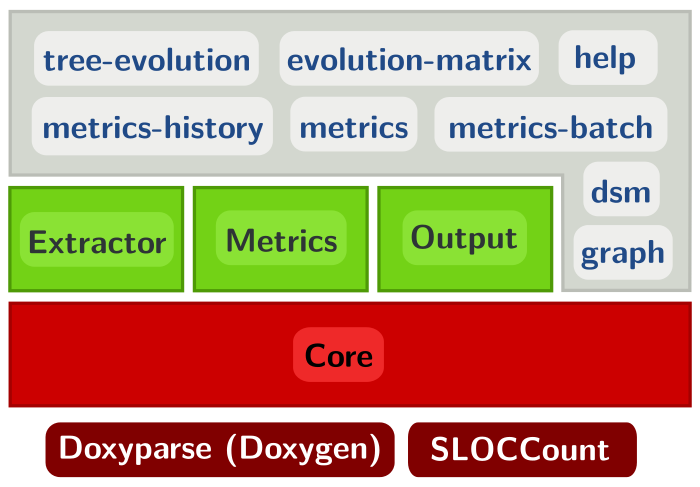
\includegraphics[scale=0.3]{imagens/analizo-architecture.png}
\caption{Arquitetura do Analizo, usando Layered Style \cite{Clements2002}}
\label{arquitetura-analizo}
\end{figure}

O {\it Core} contém as estruturas de dados usadas para armazenar informações a
respeito do código-fonte sendo analisado, como a lista de módulos\footnote{o
conceito ``módulo'' é usado como um termo abrangente para designar diferentes
tipos de estruturas usados em desenvolvimento de software, como classes e
arquivos fonte C}, elementos dentro de cada módulo (atributos, variáveis,
métodos, funções), informações de dependência (chamada, herança, etc). Esta
camada implementa a maior parte da lógica de negócio do Analizo, e não depende
de nenhuma outra camada.

A camada {\it Extractor} lida com as informaçoes de código-fonte obtidas pelas
diferentes estratégias implementadas no Analizo. Os extratores obtém
informações do código-fonte e armazenam em estruturas de dados da camada {\it
Core}. Adicionar um novo extrator requer apenas a criação de uma nova subclasse
que faça interface com uma ferramenta externa ou que ela própria realize análise
de código-fonte. Atualmente existem dois extratores, ambos fazem interface
com ferramentas externas de análise estática de código-fonte:

\begin{itemize}

  \item {\it Analizo::Extractor::Doxyparse} é uma interface para o Doxyparse,
  um parser de código-fonte para C, C++ e Java desenvolvida por nosso grupo de
  pesquisa\cite{Costa2009}. Doxyparse é baseado no
  Doxygen\footnote{doxygen.org}, um sistema de documentação multi-linguagem.

  \item {\it Analizo::Extractor::Sloccount} é uma interface para o
  Sloccount\footnote{dwheeler.com/sloccount} desenvolvido por David A. Wheeler,
  uma ferramenta que calcula o número efetivo de linhas de código.

\end{itemize}

As outras camadas intermediárias são {\it Metrics} e {\it Output}. A camada
{\it Metrics} processa as estruturas de dados do {\it Core} para calcular
métricas, até o momento Analizo suporta um conjunto razoável de métricas
(listadas na Seção \ref{metricas}). A camada {\it Output} é responsável por
lidar com diferentes formatos de arquivos. Atualmente, apenas o formato DOT é
implementado no Analizo para representar grafo de dependencia, adicionar novos
formatos é simplesmente adicionar novas classes nesta camada.

A camada {\it Tools} fornece um conjunto de ferramentas de linha de comando que
constituem a interface do analizo, tanto para usuários finais quanto para
aplicações de mais alto nível. Estas ferramentas usam serviços providos pelas
outras camadas: eles instanciam as estruturas de dados do {\it Core},
inicializam um ou mais extratores, opcionalmente executam o processador de
métricas, instanciam um módulo de formato de saída, e gerencia todos eles para
prover o resultado desejado. A maioria das funcionalidades descritas na Seção
\ref{funcionalidades} são implementadas na camada {\it Tools} do Analizo.

Estas ferramentas são pensadas na filosofia UNIX: fazem uma tarefa
especializada e geram uma saída que pode ser utilizada como entrada para outras
ferramentas, seja para o próprio Analizo ou para ferramentas externas. Algumas das
ferramentas implementadas no Analizo são feitas consumindo saída gerada por
outra ferramenta ao invés de manipular explicitamente os internos do Analizo,
algumas outras são desenhadas para prover saída em formato específico para
aplicacoes externas, como por exemplo programas para desenho de grafos ou
visualização de dados.

\section{Funcionalidades}\label{funcionalidades}

\subsection{Análise de código-fonte multi-linguagem}

Atualmente Analizo suporta análise de código-fonte escrito em C, C++ e Java.
Entretanto, pode ser facilmente estendido para suportar outras linguagens pois
pode potencialmente suportar as inúmeras outras linguagens suportadas pelo Doxygen.

\subsection{Métricas}\label{metricas}

O Analizo suporta tanto métricas em nível de projeto, que é calculada para todo o projeto,
quanto métricas em nível de módulos, que é calculado individualmente para cada módulo.
No nível de projeto, Analizo também provê estatística descritiva básica para cada métrica em
nível de módulo: soma, média, mediana, moda, desvio padrão, variância, skewness e kurtosis da
distribuição, valores mínimo e maximo. As seguintes métricas são suportadas até o momento:

\begin{itemize}

  \item Métricas em nível de projeto: Change Cost, Total Abstract Classes,
  Total Coupling Factor, Total Effective Lines of Code, Total Lines of Code,
  Methods per Abstract Class, Total Number of Modules, Total number of modules
  with at least one defined attributes, Total number of modules with at least
  one defined method, Total Number of Methods.

  \item Métricas em nível de módulo: Afferent Connections per Class, Average
  Cyclomatic Complexity per Method, Average Method Lines of Code, Argument with
  'nonnull' attribute passed null, Average Number of Parameters per Method,
  Allocator sizeof operand mismatch, Assigned value is garbage or undefined,
  Bad deallocator, Bad free, Coupling Between Objects, Dead assignment,
  Divisions by zero, Double free, Depth of Inheritance Tree, Dereference of
  null pointer, Dereference of undefined pointer value, Potential buffer
  overflow in call to 'gets', Lack of Cohesion of Methods, Lines of Code,
  Memory leak, Max Method LOC, Number of Attributes, Number of Children, Number
  of Methods, Number of Public Attributes, Number of Public Methods,
  Out-of-bound array access, Offset free, Potential insecure temporary file in
  call 'mktemp', Response for a Class, Result of operation is garbage or
  undefined, Return of stack variable address, Stack address stored into global
  variable, Structural Complexity, Undefined allocation of 0 bytes,
  Use-after-free, Uninitialized argument value.

\end{itemize}

É possível especificar que certos diretórios dentro do projeto não devem ser
analisados, de forma que o Analizo ignore tais arquivos durante a análise e o
cálculo de métricas.

\subsection{Processamento em lote}\label{lote}

A maioria dos estudos quantitativos em Engenharia de Software envolve aquisição
de métricas de código-fonte de um grande número de projetos, processar cada
projeto individualmente é pouco prático, passível de erros e difícil de
repetir. Analizo pode processar multiplos projetos em lote e produzir arquivo
de dados CSV com métricas de cada projeto, bem como um resumo com as métricas
em nível de projeto de todos os projetos. Estes arquivos de dados podem ser
facilmente importados em ferramentas de estatística ou planilhas para análise
futura. Esta capacidade de processar em lote pode também ser utilizada para
analisar várias versões de um mesmo projeto, especialmente útil em estudos
sobre evolução de software.

Este processamento em lote pode se beneficiar de processamento paralelo dando
mais agilidade e na análise e reduzindo o tempo total de processamento.  A
saída pode ser também escrita diretamente em um banco de dados relacional ao
invés de gerar arquivos CSV. Outro recurso voltado à performance é um sistema
de cache para as informações previamente calculadas, evitando repetição de
processamento.

\subsection{Histórico de métricas}

Algumas vezes pesquisadores precisam processar o histórico de projetos de
software de uma forma mais escalável. Analizo pode processar repositórios de
controle de versão e prover arquivo de dados CSV com valores de métricas para
cada revisão onde o código-fonte foi alterado no projeto, ou pode também gravar
os valores diretamente num banco de dados ao invés de usar arquivos CSV. Repositórios Git e
Subversion são suportados diretamente, repositórios CVS devem ser convertidos
para Git de forma manual.

\subsection{Grafo de dependência}

Analizo pode gerar saída com informações sobre dependência entre as entidades
do projeto em um formato adequado para processamento por ferramentas de
renderização de grafos do Graphviz\footnote{graphviz.org}. A Figura
\ref{sample-graph} apresenta um exemplo de grafo desenhado pela ferramenta {\it
dot} do Graphviz a partir da saída gerada pelo Analizo {\it graph}.

\begin{figure}[h]
\center
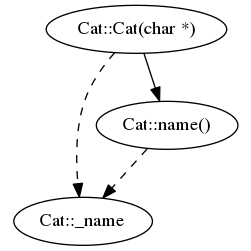
\includegraphics[scale=0.4]{imagens/sample-graph.png}
\caption{Exemplo de grafo de dependência}
\label{sample-graph}
\end{figure}

\subsection{Matriz de evolução}

Outra funcionalidade útil do Analizo é a visualização de matrizes de evolução
\cite{Lanza2001}. Ao processar cada release de um projeto (ver Seção
\ref{lote}), o usuário pode solicitar a criação de uma matrix de evolução a
partir de arquivos de dados individuais. A Figura \ref{sample-evolution-matrix}
apresenta um exemplo de uma matrix produzida pelo Analizo.

\begin{figure}[h]
\center
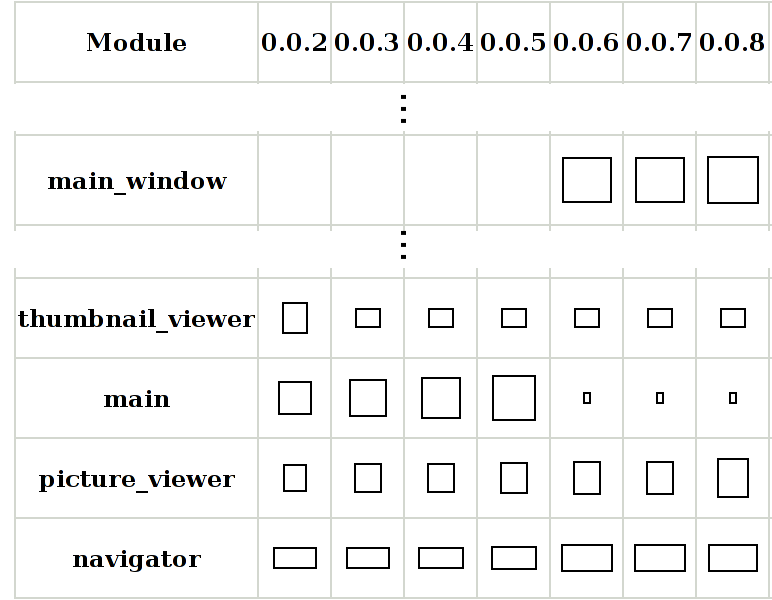
\includegraphics[scale=0.2]{imagens/sample-evolution-matrix.png}
\caption{Exemplo de matrix de evolução}
\label{sample-evolution-matrix}
\end{figure}

\subsection{Matriz de estrutura de projeto}

Uma funcionalidade recente do Analizo é a representação visual do
relacionamento entre os módulos do projeto em forma de uma Matriz de estrutura
de projeto ({\it Design Structure Matrix}) \cite{Maccormack2006}, uma DSM é a
representação de um grafo de dependência em forma de uma matriz quadrada. Um
exemplo gerado pelo Analizo pode ser visto na Figura \ref{sample-dsm}.

\begin{figure}[h]
\center
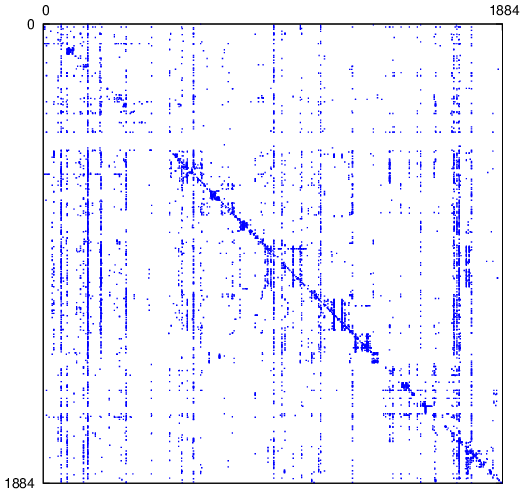
\includegraphics[scale=0.3]{imagens/sample-dsm.png}
\caption{Exemplo de matrix de estrutura de projeto}
\label{sample-dsm}
\end{figure}

\section{Uso em trabalhos de pesquisa}
\label{trabalhos-analizo}

Analizo tem sido extensivamente usada por nosso grupo de pesquisa em diversos
estudos:

\begin{itemize}

  \item \cite{Amaral2009} usou o grafo de dependencia gerado pelo Analizo para
  gerar uma matriz de evolução em um estudo de caso com o projeto VLC.

  \item \cite{Costa2009} fez uma comparação entre diferentes estratégias para
  extração de informação de dependencias entre módulos do código-fonte,
  resultando no desenvolvimento do Doxyparse - o extrator baseado no Doxygen do
  Analizo.

  \item \cite{Terceiro2009} usou métricas em um estudo exploratório sobre a
  evolução da complexidade estrutural em projetos de software livre escritos em
  C.

  \item \cite{Morais2009} usou a ferramenta de métricas do Analizo como backend
  para o Kalibro, um software para avaliação e observação de métricas de código-fonte.
  
  \item \cite{Terceiro2010} usou o processamento de histórico de métricas para
  realizar um estudo exploratório sobre a evolução da complexidade estrutural em
  7 projetos de servidor web de diferentes tamanhos.

  \item \cite{Meirelles2010} usou o processamento em lote do Analizo para
  processas o código-fonte de mais de 6000 projetos de software livre do
  repositório Sourceforge.net.

  \item \cite{Meirelles2011} usou o Analizo em um estudo sobre impacto de
  métricas de código-fonte na atratividade de projetos de softwares livres.

  \item \cite{Terceiro2012Understanding} usou o Analizo para investigar fatores
  que influenciam na evolução da complexidade estrutural em projetos de software
  livres.

  \item \cite{Silva2012} usou o Analizo para minerar 16000 revisões de
  repositórios de projetos de software para investigar o potencial de uma nova
  métrica chamada Lack of Concern-based Cohesion.

  \item \cite{Ronaldo2015} utilizou o Analizo para extrair métricas de
  código-fonte de 14 versões do sistema Android e estudar a evoluçao da API e
  seus aplicativos.

\end{itemize}

A maioria destes trabalhos contribuíram com melhorias para o Analizo, fazendo
dele ainda mais apropriado para pesquisas envolvendo análise de código-fonte.

\section{Considerações finais}

Este capítulo apresentou o Analizo, um conjunto de ferramentas para análise e
visualização de código-fonte com suporte a C, C++ e Java. Analizo é útil tanto
para pesquisadores trabalhando com análise de código-fonte quanto para
profissionais que precisam analisar seus projetos em busca de
potenciais problemas ou melhorias.

Analizo é software livre, licenciado sob a GNU General Public License versão 3.
Seu código-fonte, bem como pacotes binários, manuais e tutoriais podem ser
obtidos em http://analizo.org. Todas as ferramentas são auto-documentadas e
podem ser consultadas como páginas de manual UNIX. Analizo é escrito em Perl.


%------------------------------------------%

\xchapter{Seleção e caracterização dos projetos}
{Este capítulo apresenta ...}

A seção \ref{estudo1:introducao} apresenta ...
a seção \ref{estudo1:planejamento} apresenta o planejamento do estudo,
as seções \ref{estudo1:preparacao} e \ref{estudo1:coleta} apresentam detalhes da preparação e execução da coleta de dados,
as seções \ref{estudo1:analise} e \ref{estudo1:interpretacao} apresentam a análise e interpretação dos dados e
a seção \ref{estudo1:conclusoes} apresenta as conclusões do estudo.

% Introduction
% Background
% Experimental Setup (hipoteses / design)
% Results (data analysis)
% Discussion
% Threats to validity
% Conclusions

\section{Introdução e Motivação} \label{estudo1:introducao}

%TROUXE da INTRODUCAO e revisei. PRECISA DE CITACOES.
O software desenvolvido na academia sofre de {\it ``dysfunctional chaotic churn''} [CITAR].
Na prática, isso significa que há muitos projetos com características e funcionalidades parecidas, 
com poucos usuários, com ciclos de vida curtos, e encerrados quando o financiamento inicial termina,
bem como, comunidades desconectadas e paralelas, incompatibilidades entre projetos em um mesmo domínio, 
e tentativas aparentemente não coordenadas de ``reiniciar'' tudo ({\it re-boots}).

\section{Definição} \label{estudo1:definicao} % {{{

% Por que o estudo será realizado?

Sabemos quantos e quais são as características dos projetos de software
acadêmico de análise estática publicados em conferências de Engenharia de
Software?

\subsection{Definição do Objetivo}

\begin{description}
\item{\bf Objeto de estudo.} 
O objeto de estudo são projetos de software de análise estática publicados na literatura acadêmica.

\item{\bf Propósito.} 
O propósito é caracterizar os projetos de software de análise estática desenvolvidos na academia.

% Q: o propósito pode ser caracterizar?

\item{\bf Perspectiva.} 
A perspectiva considerada é a de cientistas usuários finais interessados em obter e utilizar software acadêmico.

\item{\bf Foco de qualidade.} 
O principal aspecto de qualidade estudado é a disponibilidade da URL para obtenção do software acadêmico.

\item{\bf Contexto.} 
O estudo foi conduzido com publicações das conferências de Engenharia de Software ASE e SCAM.

\end{description}

\subsection{Sumário da Definição}

%% GQM template

Analisar os \textit{projetos de software acadêmico de análise estática} % object of study
com o propósito de \textit{caracterizar suas informações} % purpose
com respeito a \textit{disponibilidade de URL para obtenção} % quality focus
na perspectiva de \textit{cientistas usuários finais} % perspective
no contexto de \textit{conferências de Engenharia de Software ASE e SCAM}. % context

\subsection{Questões de Pesquisa}

Neste estudo as seguintes questões de pesquisa, a respeito
%dos artigos publicados nas conferências ASE e SCAM,
dos projetos de software acadêmico de análise estática publicados nas conferências ASE e SCAM,
serão investigadas:

\newcommand{\EstudoUmQuestaoUm}{
  Quais são os projetos de software acadêmico de análise estática publicados
  com identificação de nome e URL?
}
\newcommand{\EstudoUmQuestaoDois}{
  Quantos projetos de software acadêmico de análise estática estão disponíveis
  para obtenção hoje?
}
\newcommand{\EstudoUmQuestaoTres}{
  Os projetos de software acadêmico de análise estática aceitam explicitamente
  contribuição via código fonte?
}

% Q: estas perguntas estão ok?

\begin{description}
  \item [Q1:] \EstudoUmQuestaoUm
  \item [Q2:] \EstudoUmQuestaoDois
  \item [Q2:] \EstudoUmQuestaoTres
\end{description}

\subsection{Métricas}

Para responder às questões de pesquisas, as seguintes métricas serão usadas:

\begin{enumerate}
  \item Número de artigos com publicação de software acadêmico de análise estática com identificação de nome e URL
  \item Número de projetos de software acadêmico de análise estática com URL disponível e acessível
  \item Número de projetos de software acadêmico de análise estática com código fonte disponível e com permissão explícita de contribuição via código fonte
\end{enumerate}

% }}}

\section{Planejamento do Estudo} \label{estudo1:planejamento}

Realizamos duas grandes etapas neste estudo, a primeira com objetivo de buscar
na literatura acadêmica publicações realizando contribuições em software de
análise estática, a segunda com objetivo de caracterizar os projetos a partir
de fontes documentais variadas.

\subsection{Seleção dos projetos de software acadêmico de análise estática} % {{{

A seleção dos projetos de software acadêmico de análise estática foi realizada
através de uma revisão de literatura acadêmica organizada em três etapas
distintas -- busca, filtro e seleção -- com critérios de inclusão e exclusão
utilizados para avaliar as publicações em cada etapa.

Cada etapa deste procedimento, representada na Figura
\ref{etapas-selecao-software}, produz como saída um conjunto de artigos que
atendem aos critérios de inclusão e exclusão definidos naquela etapa, estes
artigos são utilizados como entrada na etapa seguinte. A última etapa --
seleção -- gera como saída o conjunto final de artigos com publicação de
software acadêmico de análise estática.

\begin{figure}[h]
  \center
  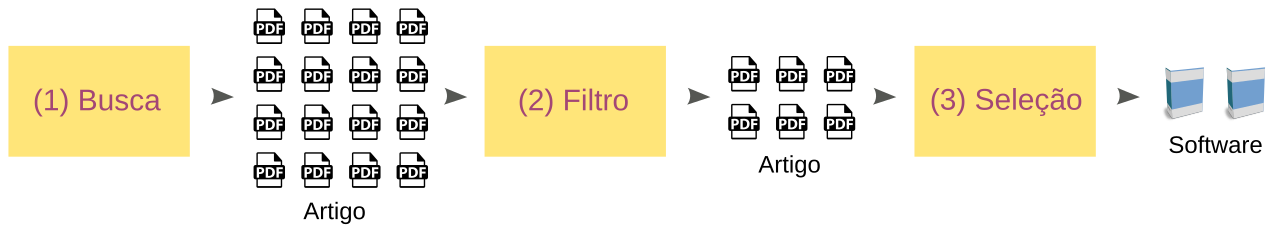
\includegraphics[scale=0.21]{imagens/etapas-selecao-software.png}
  \caption{Etapas da seleção de projetos de software acadêmico}
  \label{etapas-selecao-software}
\end{figure}

\subsubsection{Busca}

Nesta etapa definimos quais conferências serão utilizadas como fonte de busca
de software acadêmico de análise estática publicados pelos seus autores como
uma das contribuições do estudo.

A escolha de quais conferências farão parte desta etapa é realizada tendo em
vista aumentar e potencializar o número total de projetos selecionados e
busca-se conferências com histórico de publicações sobre o domínio de aplicação
do estudo, neste caso, análise estática.

Deve-se definir uma data final limite como critério de inclusão e exclusão,
sendo que a data inicial é determinada pelo histórico da conferência, devendo
englobar as edições iniciais até a última definido pela data limite.

Em casos de conferências tradicionais com longa data de existência, não é raro
que a conferência mude de nome ao longo de história, neste caso adotamos como
nome da conferência o nome mais recente e consideramos todos os outros nomes
que se passou como sendo de uma única conferência, ou seja, o nome mais
recente, mesmo que isto inclua conferencias distintas que tornaram-se uma em
algum momento.

Uma vez que estas fontes de busca estejam definidas copiamos localmente todas
as suas publicações em formato pdf até a data limite determinada, os artigos
são todos organizados em pastas por nome e ano da conferência e são também
registrados os títulos de cada artigo, além do nome da conferência e ano de
edição da conferência.

% Q: preciso dar detalhes sobre os arquivos, formato pdf, como organizei
%    em pastas, por ano, conferencia, etc?

% Q: usei libreoffice, preciso dar detalhes? fazer referencia ao nome do
%    arquivo, colunas, estrutura interna da planilha?

\subsubsection{Filtro}

A segunda etapa realiza uma busca textual automática no conteúdo de cada artigo
em seu formato pdf buscando por um conjunto de palavras chave, este conjunto
total de palavras chave é composto por subconjuntos de palavras chave
representando cada subconjunto um dos critérios de inclusão e exclusão desta
fase.

\begin{itemize}
  \item Menciona software ou ferramenta
  \item Disponibiliza online
  \item Identifica endereço
  \item Domínio de análise estática
\end{itemize}

Se um artigo não satisfaz um ou mais de um destes critérios ele é excluído do
conjunto final. Cada critério é mapeado num conjunto de strings para compor a
busca final com todos os critérios.

O principal objetivo desta etapa é reduzir o conjunto de artigos inicial,
critérios são aplicados de forma automática em cada artigo do conjunto, o
filtro automático percorre os arquivos pdf de cada artigo, aplicando uma busca
textual em todo o conteúdo, incluindo título, resumo, corpo, referências,
apêndices, anexos e demais seções do arquivo.

Assim o conjunto inicial de artigos é dividido em dois outros subconjunto, um
contendo artigos sem ocorrencia dos termos relacionados aos critérios de
interesse, e outro subconjunto, passado para a etapa seguinte, com artigos
contendo os termos pesquisados.

\subsubsection{Seleção}

Nesta etapa cada artigo deste subconjunto foi lido com objetivo de identificar
através de inspeção manual se entre as contribuições do estudo há menção a
software acadêmico de análise estática, identificado minimamente com nome e URL
para obtenção online. 
Essa leitura foi guiada pelos critérios descritos na Tabela \ref{criterios-selecao}.

% Q: tenho evitado usar o termo download, isso é necessário?

\begin{table}[h]
\caption{Critério de seleção de software acadêmico}
\centering
\begin{tabular}{ l p{12cm} }
  \hline
  Critério         & Explicação \\
  \hline
  Identificável    & É possível identificar uma contribuição em software? (ex: ``um programa que nós escrevemos``, ``nossa implementação``, ``nosso protótipo'') \\
  Disponível       & Podemos encontrar a URL do software para obtenção online (download)? \\
  \hline
\end{tabular}
\label{criterios-selecao}
\end{table}

Estes critérios foram utilizados durante a inspeção de cada artigo, sendo
realizado de forma sequencial entre cada edição de cada conferência, iniciando
pelos resultados de uma certa conferência e à seguir às demais, uma por vez, de
forma crescente, ou seja, primeiro a primeira edição de uma dada conferência,
por último a última edição, em seguida, a próxima conferência, até esgotar cada
artigo de cada conferência.

%1 seleciona um artigo do conjunto e abre o arquivo pdf deste artigo
%2 busca nome do software mencionado como de autoria desta publicação
%  se encontrar toma nota do nome, artigo, conferência e passa pro próximo passo
%  se não encontrar marca artigo como não publica software e passa pro próximo artigo
%3 busca URL e identificação sobre disponibilidade do software para obtenção
%  se encontrar toma nota da URL e passa pra próxima etapa
%  se não encontrar marca artigo como não indica fonte URL para obtenção do software
%4 registra informações sobre o artigo e sobre o projeto, seleciona próximo artigo

A inspeção manual de cada artigo foi realizado através da leitura do título,
introdução, resultados e conclusão, inicialmente, caso não seja suficiente para
identificar os critérios definidos na Tabela \ref{criterios-selecao} utilizamos
as demais seções do artigo. Alguns artigos descrevem a contribuição de software
acadêmico em seções específicas, por exemplo, é comum o uso de notas de rodapé
para indicar a URL do software.

%Q: é necessário citar o nome do software que usei para ler o PDF? Evince?

Os artigos inspecionados, tenha passado ou não nos critérios definidos aqui,
tiveram seus títulos, conferência, ano da conferência e uma informação
indicando se atenderam ou não os critérios, aqueles artigos que passaram nos
critérios, gera conjunto de projetos de software acadêmico com todos esses
dados e mais nome e URL do software, como mostra a Tabela \ref{esquema-selecao}.

\begin{table}[h]
\caption{Esquema para identificação do software na fase de seleção}
\centering
\begin{tabular}{ l p{11cm} }
  \hline
  Código                   & Explicação \\
  \hline
  Nome do software         & O nome do projeto de software \\
  URL                      & Endereço web do software ou projeto, site ou repositório de código fonte, com o software disponível \\
  Título do artigo         & Título do artigo onde o software é citado como contribuição, seja principal ou secundária \\
  Nome do evento           & Nome da conferência onde o software foi publicado \\
  Ano do evento            & Ano da edição da conferência onde o artigo foi publicado \\
  \hline
\end{tabular}
\label{esquema-selecao}
\end{table}

Os critérios de seleção da Tabela \ref{criterios-selecao} e o esquema para
identificação dos projetos de software apresentados na Tabela
\ref{esquema-selecao} foram adaptados do trabalho de
\citeonline{howison2016software}, que fez uma revisão de literatura da Biologia
em busca de menções a software acadêmico para evidenciar problemas de
visibilidade e de uso.

% }}}

\subsection{Caracterização dos projetos de software acadêmico de análise estática} % {{{

Os projetos de software acadêmico de análise estática selecionados foram então
caracterizados com informações adicionais coletadas por meio de inspeção manual
no website do projeto, de documentos, manuais e artigos. Quando o código fonte
estava disponível, o código fonte foi explorado em busca de informações sobre
licença, tipo de entrada e linguagens suportadas. Estas características são apresentadas
na Tabela \ref{esquema-caracteristicas}.

%foram coletadas 
%por meio de inspeção manual no website do projeto, de documentos, manuais e artigos.
%Quando o código fonte estava disponível, o código fonte foi explorado em busca de 
%informações sobre licença, tipo de entrada e linguagens suportadas.

\begin{table}[h]
\caption{Esquema para caracterização dos projetos de software selecionados}
\centering
\begin{tabular}{ l p{11cm} }
  \hline
  Característica           & Explicação \\
  \hline
  Descrição do software    & A descrição do projeto de software \\
  Acesso                   & Podemos acessar a URL do projeto agora? Pode receber os seguintes valores: Sem Acesso, Acesso Pago, Acesso Gratuito \\
  Distribuição             & Como o software é distribuído e pode ser acessado? Pode receber os seguintes valores: gratis, livre, proprietário \\
  Código fonte disponível  & É possível acessar o código fonte de alguma forma? \\
  Licença                  & O software deixa explícito qual licença é distribuído? \\
%  Permissão para modificar & Os criadores dão permissão para modificar o programa (se não menciona modificação, assume não)?; se permissão apenas por contato, também não \\
  Código fonte             & Em qual linguagem de programação o software acadêmico foi desenvolvido \\
  Entradas suportadas      & Qual o tipo de entrada suportada pelo software de análise estática \\
  Linguagens suportadas    & Quais linguagens de programação o software de análise estática suporta como entrada \\
  \hline
\end{tabular}
\label{esquema-caracteristicas}
\end{table}

Cada uma dessas características foram coletadas manualmente, primeiro
inspecionando o site do projeto, quando disponível, alguns projetos
disponibilizam manuais e documentos em seu site para download, estes documentos
foram consultados, normalmente arquivos txt, pdf ou doc. Quando disponível,
o código fonte também foi inspecionado em busca de informações, alguns projetos
distribuem junto ao código fonte documentos e manuais, outros documentam
algumas informações no próprio código fonte.

A característica sobre em qual linguagem de programação o projeto está escrito
foi coletado com o uso da ferramenta de software livre {\it
sloccount}\footnote{http://www.dwheeler.com/sloccount}, muitos projetos são
escritos em mais de uma linguagem, nestes casos consideramos a linguagem
dominante, o sloccount produz um resultado indicando todas as linguagens e
quanto do código total é escrito em cada uma delas.

% }}}

\section{Preparação} \label{estudo1:preparacao}

\subsection{Seleção dos projetos de software acadêmico de análise estática} % {{{

\subsubsection{Busca}

%pesquisa foram utilizadas como ponto de partida para
%selecionar o conjunto inicial de artigos: 
%O critério utilizado na definição destas fontes é bastante subjetivo 
%e depende de conhecimento prévio do pesquisador, seus pares, e colaboradores.

Seguindo o planejamento descrito em \ref{estudo1:planejamento}, definimos como
fonte de busca as conferências SCAM\footnote{\url{http://www.ieee-scam.org}}
({\it Source Code Analysis and Manipulation Working Conference}) e
ASE\footnote{\url{http://ase-conferences.org}} ({\it Automated Software
Engineering}), ambas conferências com um grande histórico de edições, ASE teve
sua primeira edição no ano de 1991 e o SCAM no ano de 2001, definimos como data
limite o ano de 2015, ou seja, incluimos os artigos publicados neste ano.

Ainda neste momento de preparação, buscamos descobrir onde estão disponíveis os
artigos de cada conferência e edição, as publicações da conferência SCAM, por
exemplo, estão todos disponibilizados no IEEE, ao menos até a data limite
investigada, já a conferência ASE, algumas edições está no IEEE outras só foram
encontradas na biblioteca digital da ACM, até o ano de 1996 a conferencia ASE
se chamava KBSE - Knowledge-Based Software Engineering Conference e a partir de
1997 passou a se chamar ASE - Automated Software Conference.

\subsubsection{Filtro}

%Dos 346 artigos do SCAM e 1533 artigos do ASE analisados na revisão estruturada
%apenas 44\% (155 artigos) e 18\% (281 artigos) continham os termos pesquisados
%no filtro automático da segunda atividade da revisão, respectivamente.

Dando sequência a preparação do estudo, definimos as palavras chave para cada
critério de filtro, como mostra a Tabela \ref{criterios-filtro}, para definir
estas palavras chave consultamos artigos com publicação de software de análise
estática e inspecionando o seu conteúdo percebemos como usualmente os
autores mencionam contribuição em software.

% Q: qual nível de detalhe eu preciso dar sobre a definição destas palavras?

\begin{table}[h]
\caption{Critérios para filtro de artigos}
\centering
\begin{tabular}{ l l }
  \hline
  Critério                        & String da busca textual               \\
  \hline
  Menciona software acadêmico     & {\tt tool} ou {\tt framework}         \\
  Disponibiliza online            & {\tt download} ou {\tt available}     \\
  Identifica endereço             & {\tt http} ou {\tt ftp}               \\
  Domínio de análise estática     & {\tt static analysis} ou {\tt parser} \\
  \hline
\end{tabular}
\label{criterios-filtro}
\end{table}

Implementamos estes critérios num script e instalamos todas as dependências
necessárias para execução, todos os detalhes de instalação e forma de uso deste
script e suas dependências de execução estão documentados no Apêndice
\ref{reproducibilidade-do-estudo}.

\subsubsection{Seleção}

Nesta fase não há preparação necessária.

% }}}

\subsection{Caracterização dos projetos de software acadêmico de análise estática} % {{{

Nesta fase de preparação para caracterização dos projetos com informações
adicionais conforme planejado, definimos o formato de armazenamendo destas
informações e quais tecnologias usar para gerenciar os dados coletados, optamos
por utilizar arquivos YAML organizados em diretórios distintos para cada
projeto de software, para coletar a informação a respeito de qual linguagem de
programação o projeto está escrito, instalamos o software livre {\it
sloccount}\footnote{http://www.dwheeler.com/sloccount}, detalhes sobre o
formato YAML, estrutura utilizada para armazenamento e instalação estão
documentados no Apêndice \ref{reproducibilidade-do-estudo}.

% }}}

\section{Coleta de Dados} \label{estudo1:coleta}

Seguindo o planejamento e preparação descritos nas seções
\ref{estudo1:planejamento} e \ref{estudo1:preparacao} iniciamos a coleta dos
dados seguindo também duas grandes etapas, uma de seleção, outra de
caracterização dos projetos de software acadêmico.

\subsection{Seleção dos projetos de software acadêmico de análise estática} % {{{

A seleção dos projetos de software acadêmico de análise estática seguiu
as etapas, conforme apresentadas na Figura \ref{etapas-selecao-software}, tomando
como primeiro passo a etapa de busca.

\subsubsection{Busca}

A busca realizada nas conferências ASE e SCAM considerando todas as edições até
o ano de 2015 resultou num conjunto total de 1873 artigos, representados na
Figura \ref{artigos-por-ano} distribuídos ao longo dos anos em cada conferência.
346 artigos do SCAM e 1527 artigos do ASE,
com uma média geral de 75 artigos publicados por ano. 

\begin{figure}[h]
  \center
  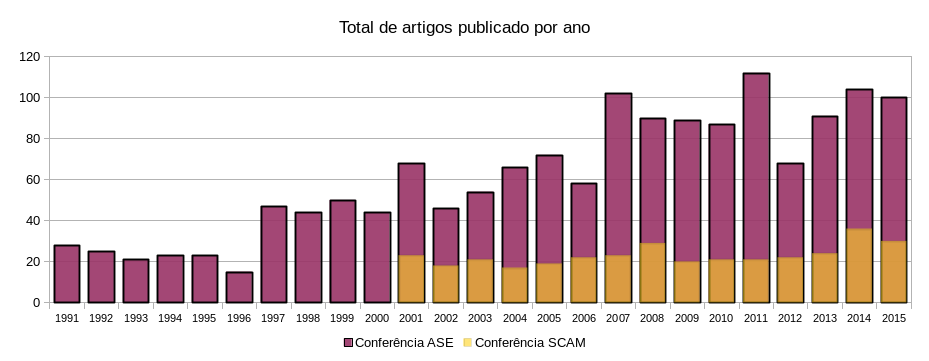
\includegraphics[scale=0.65]{imagens/artigos-por-ano.png}
  \caption{Gráfico em barras com o total de artigos publicado por ano}
  \label{artigos-por-ano}
\end{figure}

Coletamos o título de cada artigo e armazenamos juntamente com o nome da
conferência e edição onde o artigo foi publicado num arquivo do tipo ODS,
formato padrão da suíte de escritórios livre e multiplataforma
LibreOffice\footnote{\url{https://www.libreoffice.org}}, detalhes sobre este
arquivo pode ser encontrado no Apêndice \ref{reproducibilidade-do-estudo}.

\subsubsection{Filtro}

%no filtro automático da segunda atividade da revisão, respectivamente.

O filtro executado automaticamente usando os critérios definidos na fase de
preparação (seção \ref{estudo1:preparacao}) reduziu o conjunto de artigos para
441, que serão inspecionados manualmente na sequência,
155 artigos do SCAM e 286 artigos do ASE.

\subsubsection{Seleção}

Na etapa de seleção, os 441 artigos foram inspecionados, guiada pelos critérios
descritos na Tabela \ref{criterios-selecao} na fase de planejamento,
selecionados 61 artigos com publicação de software acadêmico de análise estática
segundo estes critérios, conforme Figura \ref{artigos-e-software-por-ano}
resultados distribuídos por ano.

\begin{figure}[h]
  \center
  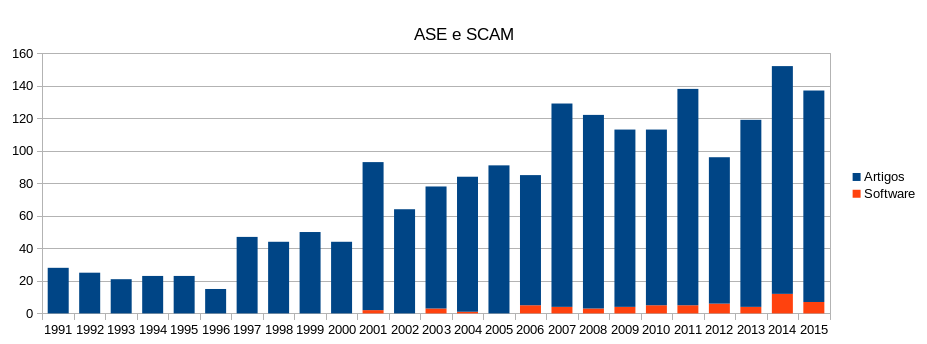
\includegraphics[scale=0.65]{imagens/artigos-e-software-por-ano.png}
  \caption{Número de projetos de software selecionados em relação ao total de publicações}
  \label{artigos-e-software-por-ano}
\end{figure}

Dois artigos, entre os 61, fazem referência a um mesmo software, assim temos no
total 60 projetos de software selecionados, para cada projeto foi criado um
diretório contendo o nome do software e um arquivo chamado
\texttt{software.yml} com os dados descritos na Tabela \ref{esquema-selecao}.

% Q: é necessário dar detalhes sobre o arquivo software.yml ?

%contribuindo com 60 projetos de software acadêmico de
%análise estática. O número de projetos de software é menor do que o número
%de artigos porque alguns foram mencionados em mais de um artigo. 

% }}}

\subsection{Caracterização dos projetos de software acadêmico de análise estática} % {{{

Conforme planejado coletamos informações adicionais para cada projeto de
software selecionado, as informações descritas na Tabela
\ref{esquema-caracteristicas} foram coletadas,

%por meio de inspeção manual no website do projeto, de documentos, manuais e artigos.
%Quando o código fonte estava disponível, o código fonte foi explorado em busca de 
%informações sobre licença, tipo de entrada e linguagens suportadas.

%Para identificar a linguagem de programação em que o software foi escrito, utilizamos a
%ferramenta livre {\it sloccount}\footnote{http://www.dwheeler.com/sloccount}.

% }}}

% \section{Operação} %%%%%%%%

% Raw results from the analysis
\section{Análise dos Dados} \label{estudo1:analise}

Dados de 60 projetos de software acadêmico de análise estática desenvolvidos e
publicados na literatura acadêmica de engenharia de software, nas conferências
ASE e SCAM, até o ano de 2015, informaçoes sobre as formas de distribuição e
licenciamento, dados de acesso ao software.

% ATENCAO: parei aqui, proximo passo:

% * criar template para gerar uma tabela e substituir a tabela (temporaria)
%   incluida abaixo
% * exibir nesta tabela as seguintes colunas para cada software:
%   - nome do software
%   - distribuição
%   - disponível para download?
%   - código fonte disponível?
%   - licença
%   - código fonte
\begin{longtable}{| l | c | c | c | c | c | c |}
\caption{Software acadêmico para análise estática.}
\label{tab:software} \\ 
  \hhline{| l | c | c | c | c | c | c |} \hline \endfirsthead
  %\hhline{|-------|} \multicolumn{7}{|c|}{continuação da página anterior} \\ \hline
  \hhline{| l | c | c | c | c | c | c |} \hline \textbf{Software} & \textbf{Versões} & \textbf{Citações} & \textbf{[cita]} & \textbf{[usa]} & \textbf{[contribui]} & \textbf{[cria]} \\ \hline
  \hhline{| l | c | c | c | c | c | c |}  \endhead
  \hhline{|-------|} \multicolumn{7}{|c|}{continua na próxima página} \\ \hline
  \hhline{|-------|} \endfoot
  \hhline{|-------|} \endlastfoot
\textbf{Software} & \textbf{Versões} & \textbf{Citações} & \textbf{[cita]} & \textbf{[usa]} & \textbf{[contribui]} & \textbf{[cria]} \\ \hline
  2ls
  &
  7
  &
  1
  &
  0
  &
  0
  &
  0
  &
  1
  \\
  accessanalysis
  &
  4
  &
  2
  &
  1
  &
  0
  &
  0
  &
  1
  \\
  apiexample
  &
  0
  &
  4
  &
  3
  &
  0
  &
  0
  &
  1
  \\
  beg
  &
  0
  &
  9
  &
  4
  &
  3
  &
  1
  &
  1
  \\
  ccjava
  &
  0
  &
  5
  &
  1
  &
  0
  &
  3
  &
  1
  \\
  civl
  &
  36
  &
  6
  &
  5
  &
  0
  &
  0
  &
  1
  \\
  codeboost
  &
  134
  &
  15
  &
  14
  &
  0
  &
  0
  &
  1
  \\
  composite
  &
  0
  &
  6
  &
  2
  &
  2
  &
  1
  &
  1
  \\
  cpa+
  &
  0
  &
  5
  &
  0
  &
  0
  &
  4
  &
  1
  \\
  cseq
  &
  0
  &
  5
  &
  1
  &
  2
  &
  1
  &
  1
  \\
  ddverify
  &
  0
  &
  3
  &
  2
  &
  0
  &
  0
  &
  1
  \\
  derailer
  &
  2
  &
  2
  &
  1
  &
  0
  &
  0
  &
  1
  \\
  diagnosys
  &
  0
  &
  1
  &
  0
  &
  0
  &
  0
  &
  1
  \\
  dompletion
  &
  0
  &
  2
  &
  1
  &
  0
  &
  0
  &
  1
  \\
  drc
  &
  0
  &
  5
  &
  4
  &
  0
  &
  0
  &
  1
  \\
  e-munity
  &
  0
  &
  1
  &
  0
  &
  0
  &
  0
  &
  1
  \\
  ejb
  &
  0
  &
  3
  &
  1
  &
  1
  &
  0
  &
  1
  \\
  error-prone
  &
  22
  &
  2
  &
  0
  &
  1
  &
  0
  &
  1
  \\
  esbmc
  &
  0
  &
  42
  &
  16
  &
  18
  &
  7
  &
  1
  \\
  etxl
  &
  0
  &
  1
  &
  0
  &
  0
  &
  0
  &
  1
  \\
  faultbuster
  &
  0
  &
  1
  &
  0
  &
  0
  &
  0
  &
  1
  \\
  flowgen
  &
  0
  &
  3
  &
  2
  &
  0
  &
  0
  &
  1
  \\
  grt
  &
  0
  &
  9
  &
  4
  &
  2
  &
  3
  &
  0
  \\
  guizmo
  &
  0
  &
  1
  &
  0
  &
  0
  &
  0
  &
  1
  \\
  gumtree
  &
  3
  &
  18
  &
  5
  &
  11
  &
  1
  &
  1
  \\
  husacct
  &
  22
  &
  7
  &
  3
  &
  2
  &
  0
  &
  2
  \\
  indus
  &
  36
  &
  4
  &
  0
  &
  3
  &
  0
  &
  1
  \\
  jastadd
  &
  24
  &
  43
  &
  24
  &
  15
  &
  3
  &
  1
  \\
  jflow
  &
  5
  &
  7
  &
  5
  &
  1
  &
  0
  &
  1
  \\
  jstereocode
  &
  0
  &
  8
  &
  2
  &
  5
  &
  0
  &
  1
  \\
  jtop
  &
  0
  &
  2
  &
  0
  &
  1
  &
  0
  &
  1
  \\
  kiasan
  &
  0
  &
  16
  &
  10
  &
  0
  &
  5
  &
  1
  \\
  loopfrog
  &
  0
  &
  5
  &
  2
  &
  2
  &
  0
  &
  1
  \\
  lotrack
  &
  0
  &
  2
  &
  1
  &
  0
  &
  0
  &
  1
  \\
  mpanalyzer
  &
  0
  &
  1
  &
  0
  &
  0
  &
  0
  &
  1
  \\
  msp
  &
  0
  &
  2
  &
  1
  &
  0
  &
  0
  &
  1
  \\
  mygcc
  &
  5
  &
  7
  &
  3
  &
  1
  &
  1
  &
  2
  \\
  parseweb
  &
  0
  &
  24
  &
  22
  &
  1
  &
  0
  &
  1
  \\
  pat
  &
  0
  &
  2
  &
  1
  &
  0
  &
  0
  &
  1
  \\
  php-air
  &
  4
  &
  9
  &
  1
  &
  5
  &
  2
  &
  1
  \\
  protopurity
  &
  0
  &
  1
  &
  0
  &
  0
  &
  0
  &
  1
  \\
  pseudogen
  &
  0
  &
  1
  &
  0
  &
  0
  &
  0
  &
  1
  \\
  ptyasm
  &
  0
  &
  2
  &
  0
  &
  0
  &
  2
  &
  0
  \\
  pumoc
  &
  0
  &
  2
  &
  1
  &
  0
  &
  0
  &
  1
  \\
  pythia
  &
  0
  &
  2
  &
  0
  &
  0
  &
  1
  &
  1
  \\
  reassert
  &
  5
  &
  13
  &
  9
  &
  3
  &
  0
  &
  1
  \\
  reve
  &
  0
  &
  1
  &
  0
  &
  0
  &
  0
  &
  1
  \\
  rrfinder
  &
  0
  &
  3
  &
  2
  &
  0
  &
  0
  &
  1
  \\
  sapid-xml
  &
  0
  &
  5
  &
  1
  &
  2
  &
  1
  &
  1
  \\
  sonarqube-plugin
  &
  4
  &
  1
  &
  0
  &
  0
  &
  0
  &
  1
  \\
  sparta
  &
  14
  &
  4
  &
  1
  &
  2
  &
  0
  &
  1
  \\
  srcml
  &
  14
  &
  40
  &
  14
  &
  23
  &
  2
  &
  1
  \\
  swat
  &
  0
  &
  4
  &
  1
  &
  2
  &
  0
  &
  1
  \\
  tacle
  &
  0
  &
  3
  &
  1
  &
  1
  &
  0
  &
  1
  \\
  teba
  &
  21
  &
  1
  &
  0
  &
  0
  &
  0
  &
  1
  \\
  testera
  &
  0
  &
  23
  &
  17
  &
  5
  &
  0
  &
  1
  \\
  vdiff
  &
  0
  &
  5
  &
  4
  &
  0
  &
  0
  &
  1
  \\
  wala
  &
  37
  &
  11
  &
  5
  &
  5
  &
  0
  &
  1
  \\
  wrangler
  &
  34
  &
  33
  &
  16
  &
  10
  &
  6
  &
  1
  \\
  xogastan
  &
  0
  &
  5
  &
  4
  &
  0
  &
  0
  &
  1
  \\
  \hline
\end{longtable}




% Hypothesis rejection
\section{Interpretação dos Resultados} \label{estudo1:interpretacao}

\subsection{Q1 - \EstudoUmQuestaoUm} % {{{

Até o ano de 1996 a conferencia ASE chamava-se KBSE\footnote{ Knowledge-Based
Software Engineering Conference} e só a partir de 1997 mudou para ASE, a
conferência SCAM teve sua primeira edição apenas em 2001, 10 anos após a
primeira edição do ASE.

No geral, a conferência ASE publica quase 4 vezes mais do que a conferência
SCAM, a edição com o maior número de publicações foi 2011 com 112 artigos
publicados, seguido de 2014 com 104, e 2007 com 102, a edição com o menor
número foi 1996 com apenas 15 artigos publicados.

Detalhes sobre o número de artigos
em cada conferência pode ser consultados nos Apêndices
\ref{artigos-do-scam} e \ref{artigos-do-ase} 

%Situação similar ocorreu com o {\it Augmenting
%Counterexample-Guided Abstraction Refinement with Proof Templates} e o {\it
%PtYasm: Software Model Checking with Proof Templates} publicados no ASE 2008,
%fazem referência ao software PtYasm. 
%Por conta disso, entre os 107 artigos, 

%Ainda durante esta última atividade da revisão cada um dos 107 artigos foram
%analisados em busca de informações sobre onde encontrar o software indicado,

Resultou em 60 softwares com indicação de fonte para obtenção do
software, apenas os artigos que indicam endereço de página web para download do
software foram selecionados, ou seja, uma grande parte dos artigos que produzem
softwares acadêmicos nem ao menos citam o software no paper, ou quando citam,
não informam site ou endereço do projeto para download
\cite{allen2017engineering}, seja código fonte ou apenas binários.


É possível perceber um crescimento no número de software publicados com o
passar dos anos, de forma que podemos confirmar que considerando as
conferências ASE e SCAM, há um crescimento na publicação de softwares
acadêmicos ao longo do tempo.

Apesar da busca na atividade -- (2) Filtro -- utilizar termos com o objetivo de
encontrar apenas softwares disponíveis com informação de onde encontrar o
software, ainda assim, encontramos 45 artigos com publicação de software sem
indicação de fonte para obtenção.

Entre os 1873 artigos, encontramos 107 artigos referenciando 105 softwares de
análise estática, apenas 60 destes indicam a fonte onde o software pode ser
encontrado.

% }}} Q1

\subsection{Q2 - \EstudoUmQuestaoDois} % {{{

%\citeonline{robles2010replicating} afirma que existe uma tendência das páginas
%web onde os softwares estão disponíveis tem uma grande chance de se tornarem
%indisponíveis ao passar do tempo, investigamos esta tendência 
%cruzando a informação de acesso ao software com a data de publicação do paper
%onde o software foi selecionado.
%a Figura \ref{softwares-disponivel-por-ano} apresenta em cada ano quantos
%porcentos do total de softwares publicados ainda continuam
%disponíveis hoje.

Apenas 37 estão disponíveis, os 23 restantes indicam fonte não mais
acessíveis, endereço não encontrado, indisponível, ou com informações não
relacionadas ao software. 
O Apêndice \ref{resumo-softwares-disponiveis} traz
uma tabela com os nomes e endereços web onde os softwares estão disponíveis.

%Levando em conta a sustentabilidade técnica podemos responder que 
Observamos que 61\% do software acadêmico produzido no domínio de aplicação de análise estática 
são sustentáveis, ou seja, continuam disponíveis ao longo do tempo. 
É importante destacar que não foram considerados aqui artigos que publicaram software 
sem menção à fonte onde o mesmo poderia ser encontrado.
% a revisão estruturada teve como foco encontrar artigos com publicação softwares com indicação de fonte,
% ou seja, aqueles artigos que publicam software mas que não indicam fonte não está sendo
% considerado aqui, vimos que na revisão estruturada, mesmo não sendo o objetivo
Se os artigos que não indicaram a fonte onde o software acadêmico poderia ser encontrado
fossem incluídos -- 45 artigos sem informação de fonte --, 
a taxa de sustentabilidade cairia para apenas 35\%.
Uma revisão estruturada mais abrangente, que desconsiderasse o critério de exclusão
(indicar fonte do software acadêmico), possivelmente resultaria em taxas abaixo dos 35\%, 
sugerindo que a quantidade de software acadêmico publicado em artigos porém indisponível para acesso
pode ser maior do que a encontrada neste estudo.

%TRABALHO FUTURO
%\citeonline{robles2010replicating} afirma que as páginas
%web onde os projetos de software acadêmico foram publicados 
%se tornem indisponíveis com o passar do tempo.
%Podemos investigar esta tendência avaliando os 60 softwares com fonte indicada no artigo,
%identificar se confirmamos neste contexto se com a idade do paper
%as páginas web onde os softwares são publicados tem uma grande chance de se
%tornarem indisponíveis ao passar do tempo.

\begin{figure}[h]
  \center
  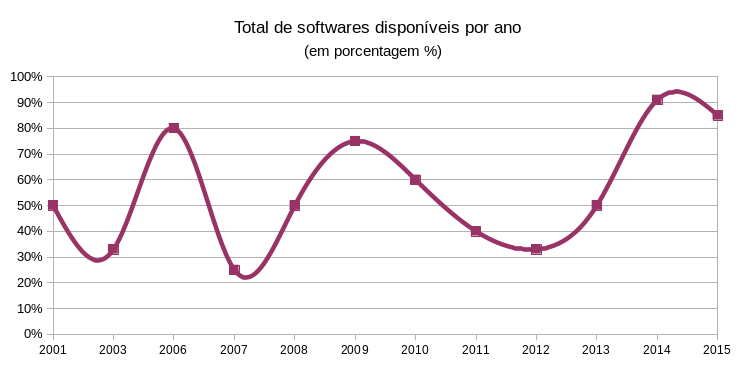
\includegraphics[scale=0.65]{imagens/softwares-disponivel-por-ano.png}
  \caption{Gráfico em linha com o total de projetos de software acadêmico disponíveis por ano}
  \label{softwares-disponivel-por-ano}
\end{figure}

A Figura \ref{softwares-disponivel-por-ano} apresenta 
um gráfico em linha com o total de projetos de software acadêmico disponíveis por ano.
Também apresenta a porcentagem de software acadêmico publicado com indicação de fonte que ainda estão
disponíveis, ou seja, a taxa de projetos de software que continuam
disponíveis hoje, considerando o conjunto de projetos de software publicado em cada ano 
com informação sobre fonte para download. 
Os anos de 2002, 2004, 2005, e anteriores a 2001 não possuem software publicado
com fonte indicada no artigo ainda disponível e, portanto,
suas informações não aparecem no gráfico.

Ao analisar a Figura \ref{softwares-disponivel-por-ano},
percebemos que há um leve crescimento na disponibilidade
dos projetos de software acadêmico  nos anos mais recentes.
%
Existe uma leve tendência, ao longo dos anos,  
para a indisponibilidade das fontes informadas e páginas web.
É possível notar que, em 2006, 80\% de todos os
softwares de análise estática publicados nas conferências ASE e SCAM ainda estão disponíveis.
Este número cresce em 2014, chegando a 90\%, e cai no ano seguinte para 85\%.
Apesar de não estar sempre crescente, e da  amostra pequena usada neste estudo 
-- apenas 60 projetos de software acadêmico,
este leve indício confirma a afirmação de \citeonline{robles2010replicating}.

Os 37 softwares com fonte disponível foram avaliados em relação ao segundo
aspecto, isto é, com respeito à forma em que estão disponíveis:
se os artigos informam onde obter tais softwares, se os softwares estão realmente disponíveis, e 
se, ao acessar as fontes indicadas na presente data deste estudo, os softwares estão funcionando e
acessíveis.

Do conjunto de 37 projetos de software estudados, %% Joenio, coloquei aqui o tempo no PRETERITO -- revisar outras partes.
3 não disponibilizaram seu código fonte e  %% Joenio, mudei as frases para VOZ ativa, sujeito: projeto de software.
34 disponibilizaram o código fonte publicamente.
Dentre os que disponibilizaram o código fonte, 13 não informaram licença alguma
%apesar de ter o código fonte disponível, 
e 21 informaram licenças de FOSS ({\it free and open source software}):

\begin{itemize}
  \item 8 usam GNU General Public License;
  \item 2 usam Apache License;
  \item 4 usam BSD License;
  \item 3 usam Eclipse Public License;
  \item 2 usam University of Illinois/NCSA Open Source License;
  \item 1 usa licença {\it FrontEndART Software Ltd}; e
  \item 1 usa licença {\it SAnToS Laboratory Open Academic License}.
\end{itemize}

Entre os 37 softwares disponíveis, 21 podem ser modificados para se adaptar às
necessidades emergentes sem necessidades de solicitação prévia de autorização
aos autores originais devido ao uso de licenças livres. 
Os 13 softwares restantes com código fonte disponível mas sem licença expressa podem
ser modificados, mas a falta de uma licença impõe a necessidade
de solicitar permissão aos autores originais.

35\% dos softwares disponíveis podem ser adaptados de forma incremental para
aproveitar oportunidades emergentes, 21\% podem mediante prévia autorização do
autor original serem modificados, e apenas 5\% não oferecem essa possibilidade
por não disponibilizarem o código fonte publicamente.

%4º Princípio, Persistencia.    % ??????

Os identificadores únicos e metadados descrevendo o software e sua disposição
devem persistir - mesmo além do tempo do software que descrevem.

%Deste total apenas 11\% (41 artigos) e 4\% (62 artigos) foram selecionados na
%terceira e última atividade da revisão contendo publicação de ferramenta de
%análise estática.

%Resultando em 103 artigos com publicação de {\it software científico} de
%análise estática de código fonte, apenas 35 possuem fonte para obtenção do
%software, sendo 32 de código aberto, ou seja, com disponibilidade de
%código fonte, e 3 grátis, apenas binários disponível. Ou seja, apenas 31\% dos
%artigos com publicação de software disponibilizam o código fonte das mesmas.
%Isto significa que 69\% dos artigos com publicação de software de análise
%estática de código fonte são potencialmente impossíveis de serem repetidos, já
%que os artefatos originais são necessários para tal atividade e o artigo não
%disponibiliza o código fonte dos mesmos.

% }}} Q2

\subsection{Q3 - \EstudoUmQuestaoTres} % {{{

Número de menções a cada software acadêmico e qual o contexto e tipo de menção
é feita, quem e quantos são os autores de cada menção.

...

%cada citação pontua no máximo 1 ponto para o peso final do paper ao quanto
%contribui para a sustentabilidade técnica do software, esta pontuação será
%calculada com base nos pesos (em porcentagem) 'contribution\_weight' e
%'authorship\_weight', este último valor é aplicado à contribution weight,
%ou seja contribution\_weight é acrescido a partir do valor de authorship\_weight.
%o valor final se ultrapassar 1 será cortado no limite 1 (máximo), a ideia não é muito
%os números, não queremos saber se são numeros altos, queremos constancia, queremos
%medir se existe um nível de contribuição mínimo aos softwares, isto está
%sendo proposto como algo que mantém o software vivo e útil para a comunidade
%acadêmmica. (por hora o valor mínimo "ideal" por ano é "0.5", ou seja, um
%valor bem modesto, este valor indica que houve ao menos uma contribuição
%ao software, ou que teve citações suficientes equivalente a uma contribuição,
%o software ao ser muito citado ganha mais visibilidade, impacta na possibilidade
%de maior adoção e maior contribuição por terceiros.

% }}} Q3

\subsection{Ameaças à validade}

Validade de construção.
A leitura dos artigos na revisão estruturada para identificar se publicam
softwares de análise estática de código fonte, se disponibilizam fonte para
obtenção de tais softwares, e se os softwares são mesmo do domínio de aplicação
de análise estática de código fonte podem ter maior validade se feitos em
par e revisados por outros pesquisadores.
Neste estudo, estas atividades foram realizadas pelo autor desta dissertação e 
não houve revisão por pesquisadores independentes.
%% A ameaça não foi tratada.

Validade externa. Apenas duas conferências. Apenas duas bases. Apenas um domínio de software acadêmico / uma área do conhecimento em que pesquisadores também programam.
%% A ameaça não foi tratada.

etapa busca: Sabemos que no subconjunto excluído, por ser automático, poderá existir artigos
dentro dos critérios mencionados, com publicação de software, mas 

\section{Conclusões} \label{estudo1:conclusoes}

FALTA uma síntese aqui. 
Este estudo ...
Resultados mostram que ...
Algumas tendências emergiram a partir da leitura ...

Planejamos fazer outro estudo ... 

\xchapter{Análise do ciclo de vida dos projetos}
{Este capítulo apresenta ...}

A seção \ref{sec:study1:intro} apresenta ...
seção \ref{sec:study1:definition} ...
seção \ref{sec:study1:operation} ...

% Introduction
% Background
% Experimental Setup (hipoteses / design)
% Results (data analysis)
% Discussion
% Threats to validity
% Conclusions

\section{Introdução e Motivação} \label{sec:study1:intro}

%TROUXE da INTRODUCAO e revisei. PRECISA DE CITACOES.
O software desenvolvido na academia sofre de {\it ``dysfunctional chaotic churn''} [CITAR].
Na prática, isso significa que há muitos projetos com características e funcionalidades parecidas, 
com poucos usuários, com ciclos de vida curtos, e encerrados quando o financiamento inicial termina,
bem como, comunidades desconectadas e paralelas, incompatibilidades entre projetos em um mesmo domínio, 
e tentativas aparentemente não coordenadas de ``reiniciar'' tudo ({\it re-boots}).

\textbf{O caso do Analizo.}  Descrever uma situação em que software acadêmico foi necessário
para apoiar pesquisa. egypt, etc. analizo, comunidade, usp, etc.
menções ...

Analizo \cite{Terceiro2010Analizo} é um conjunto de ferramentas para análise de código-fonte e
visualização com suporte a múltiplas linguagens de programação, software livre,
extensível e capaz de lidar com código-fonte não mais compilável. A capacidade
de lidar com código-fonte não mais compilável permite analisar código-fonte
com erros de sintaxe, com referências a bibliotecas não mais disponíveis, ou
que usem bibliotecas com mudanças de API.

Analizo tem sido extensivamente usado por nosso grupo de pesquisa em diversos
estudos.
\cite{Amaral2009} usou o grafo de dependencia gerado pelo Analizo para
  gerar uma matriz de evolução em um estudo de caso com o projeto VLC.
\cite{Costa2009} fez uma comparação entre diferentes estratégias para
  extração de informação de dependencias entre módulos do código-fonte,
  resultando no desenvolvimento do Doxyparse - o extrator baseado no Doxygen do
  Analizo.
\cite{Terceiro2009} usou métricas em um estudo exploratório sobre a
  evolução da complexidade estrutural em projetos de software livre escritos em
  C.
\cite{Morais2009} usou a ferramenta de métricas do Analizo como backend
  para o Kalibro, um software para avaliação e observação de métricas de código-fonte.
\cite{Terceiro2010} usou o processamento de histórico de métricas para
  realizar um estudo exploratório sobre a evolução da complexidade estrutural em
  7 projetos de servidor web de diferentes tamanhos.
\cite{Meirelles2010} usou o processamento em lote do Analizo para
  processas o código-fonte de mais de 6000 projetos de software livre do
  repositório Sourceforge.net.
\cite{Meirelles2011} usou o Analizo em um estudo sobre impacto de
  métricas de código-fonte na atratividade de projetos de softwares livres.
\cite{Terceiro2012Understanding} usou o Analizo para investigar fatores
  que influenciam na evolução da complexidade estrutural em projetos de software
  livres.
\cite{Silva2012} usou o Analizo para minerar 16000 revisões de
  repositórios de projetos de software para investigar o potencial de uma nova
  métrica chamada Lack of Concern-based Cohesion.

% \cite{Ronaldo2015}

% \cite{Mateus2017}

A maioria destes trabalhos contribuíram com melhorias para o Analizo, fazendo
dele uma ferramenta bastante apropriada para pesquisas envolvendo análise de código-fonte,
sendo útil tanto para pesquisadores trabalhando com análise de código-fonte
quanto para profissionais que precisam analisar seus projetos em busca de
potenciais problemas ou melhorias.

Analizo é software livre, distribuído sob a licença GNU General Public License
versão 3. Seu código-fonte, bem como pacotes binários, manuais e tutoriais
podem ser obtidos em \url{http://www.analizo.org}. Todas as ferramentas são
auto-documentadas e podem ser consultadas como páginas de manual UNIX. Analizo
é escrito em Perl, sua última versão 1.19.1 lançada em 01 de Setembro de 2016
foi a versão utilizada neste estudo.


% TRAZER/USAR o termo ecossistema de software aqui?
% Creio que o termo ```projeto'' atende ... a discutir.
% Como usar outros elementos do ecossistema neste capitulo, por exemplo, atores?
% Sustentabilidade técnica para a ciência de um modo geral?  ou sócio-técnica?


\section{Definição} \label{sec:study1:definition}

% Por que o estudo será realizado?

O que sabemos sobre a sustentabilidade técnica de projetos de software acadêmico publicados em conferências
de Engenharia de Software? Como estes projetos são mencionados na literatura acadêmica?   
Colocar QUESTAO SOBRE COLABORACAO.


\subsection{Definição do Objetivo}

\begin{description}
\item{\bf Objeto de estudo.} 
O objeto de estudo são projetos de software acadêmico de análise estática e sua sustentabilidade técnica.

\item{\bf Propósito.} 
O propósito deste estudo é caracterizar a sustentabilidade técnica de cada software acadêmico de análise estática,
trazendo informações que permitam ...

\item{\bf Perspectiva.} 
A perspectiva considerada é a de cientistas e pesquisadores, isto é, 
o cientista ou pesquisador gostaria de conhecer ecossistemas de software acadêmico de análise estática
em termos de sua sustentabilidade técnica. 
Além disso, pessoas da indústria podem estar interessadas em conhecer
software acadêmico de análise estática para financiá-lo.

\item{\bf Foco de qualidade.} 
O principal aspecto de qualidade estudado é a sustentabilidade sócio-técnica,
com destaque para três aspectos: transparência, complexidade e adoção.
%, A, B, C ... EXPLICAR A, B, C.


Q1 é demográfica?
Transparência: aberto? disponível? transparente?  Funciona? Ver Q2.
Adoção: ver Q4.
Q3? Parece que há duas questões em uma. Você vai olhar todas as versões para tratar da visibilidade??
A outra questão tem a ver sobre como referenciar software em artigos científicos?
Complexidade: qualidade do código.  Estudo 2.

\item{\bf Contexto.} 
O estudo foi conduzido com projetos de software acadêmico de análise estática
publicados nas conferências ASE e SCAM.
\end{description}

\subsection{Sumário da Definição}

%% QUERO DISCUTIR SE SUSTENTABILIDADE JA EH MENCIONADA OU NAO no Object of Study

%% GQM template

Analisar a \textit{software acadêmico de análise estática e sua sustentabilidade técnica} % object of study
com o propósito de \textit{caracterizar}  % purpose  % era medir e avaliar - coloquei 'caracterizar' 
com respeito a \textit{disponibilidade de código, números de citações e complexidade estrutural (manutenibilidade)}  % quality focus
na perspectiva do \textit{pesquisador} e do \textit{cientista}% perspective
no contexto de \textit{software acadêmico de análise estática publicado nas conferências ASE e SCAM 
e referenciado por artigos publicados nas bases da ACM e IEEE}. % context
%


\subsection{Questões de Pesquisa}

Neste estudo as seguintes questões de pesquisa, a respeito do ecossistema de
software acadêmico de análise estática, serão investigadas:

\newcommand{\EstudoDoisQuestaoUm}{Como as taxas de publicação contribuindo com novos projetos de software acadêmico nas conferências ASE e SCAM mudam ao longo do tempo?}
\newcommand{\EstudoDoisQuestaoDois}{Os projetos estão disponíveis para obtenção hoje? Os projetos incentivam ativamente a contribuição? Os espaços do projeto são abertos e transparentes?}
\newcommand{\EstudoDoisQuestaoTres}{Como a visibilidade dos artefatos de software publicados nas conferências ASE e SCAM mudam ao longo do tempo? Como os artefatos de software acadêmico publicados nas conferências ASE e SCAM são mencionados na literatura acadêmica ao longo do tempo?}
\newcommand{\EstudoDoisQuestaoQuatro}{Como as taxas de entrada de novos atores cientistas usuários finais de software acadêmico mudam ao longo do tempo? Os projetos possuem contribuidores além dos autores iniciais?}

\begin{description}
  \item [Q1:] \EstudoDoisQuestaoUm
  \item [Q2:] \EstudoDoisQuestaoDois
  \item [Q3:] \EstudoDoisQuestaoTres
  \item [Q4:] \EstudoDoisQuestaoQuatro
\end{description}

%\subsection{Resultados}

%\begin{enumerate}
%  \item Caracterização do ecossistema de software acadêmico de análise estática
%  \item Reflexão sobre os problemas de sustentabilidade sofridos pelo ecossistema de software acadêmico de análise estática
%  \item Formulação de hipóteses sobre os problemas de sustentabilidade sofridos pelo ecossistema de software acadêmico de análise estática
%\end{enumerate}

\subsection{Métricas}

Para responder às questões de pesquisas, as seguintes métricas serão usadas:
\begin{enumerate}
\item métricas relacionadas ao ecossistema do software (número
total de lançamentos, data e número de versão de cada lançamento, número de
commits, número de contribuidores); % estudo2
\item métricas relacionadas à qualidade interna do software (complexidade estrutural do código fonte). % estudo3
\item métricas de publicação (número de citações, número de menções, número de usos).) %estudo2
\end{enumerate}

%\section{Planejamento do Estudo} \label{sec:study1:planning}

% Como o estudo será conduzido?

\section{Coleta de dados} \label{sec:study1:operation}

A população estudada compreende um conjunto de 60 projetos de software
acadêmico de análise estática publicados na literatura acadêmica de engenharia
de software.

\subsection{Seleção de software acadêmico}

O contexto deste estudo inclui um conjunto de projetos de software acadêmico ...

A seleção de software acadêmico seguiu um procedimento
composto de 3 etapas -- busca, filtro e seleção.
Cada etapa deste procedimento, representada na Figura \ref{figura-revisao-estruturada}, gera
como saída um conjunto de artigos utilizado como entrada na etapa seguinte.
A última etapa -- seleção -- gera como saída a nossa população de 60 projetos.

\subsubsection{Busca}

Para a etapa de busca, duas fontes de pesquisa foram utilizadas como ponto de partida para
selecionar o conjunto inicial de artigos: 
%O critério utilizado na definição destas fontes é bastante subjetivo 
%e depende de conhecimento prévio do pesquisador, seus pares, e colaboradores.
a conferência SCAM - {\it Source Code Analysis and
Manipulation Working Conference}\footnote{\url{http://www.ieee-scam.org}} e 
a conferência ASE - {\it Automated Software Engineering}\footnote{\url{http://ase-conferences.org}},
ambas com histórico de publicações sobre análise de programas.
Incluimos todas as edições das duas conferências até o ano de 2015.

A busca resultou em um conjunto inicial de 1873 artigos,
todos copiados localmente em formato pdf e organizados em diretórios, por conferência
e ano de edição.
A Figura \ref{artigos-por-ano} apresenta o total de artigos distribuído
por ano para cada conferência.

\begin{figure}[h]
  \center
  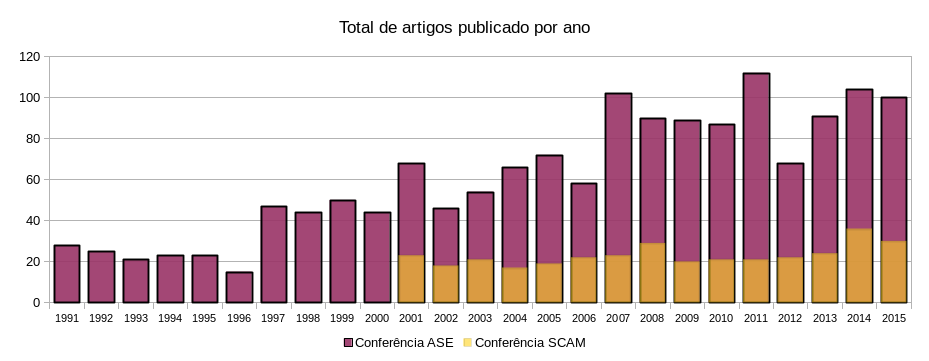
\includegraphics[scale=0.65]{imagens/artigos-por-ano.png}
  \caption{Gráfico em barras com o total de artigos publicado por ano}
  \label{artigos-por-ano}
\end{figure}

\subsubsection{Filtro}

%Dos 346 artigos do SCAM e 1533 artigos do ASE analisados na revisão estruturada
%apenas 44\% (155 artigos) e 18\% (281 artigos) continham os termos pesquisados
%no filtro automático da segunda atividade da revisão, respectivamente.

A segunda etapa filtra o conjunto total de artigos mantendo apenas aqueles que
combinam com os critérios definidos na Tabela \ref{codes-for-filter}, estes
critérios são aplicados de forma automática em cada artigo do conjunto, se um
artigo não satisfaz um ou mais de um destes critérios ele é excluído do
conjunto final.

\begin{table}[h]
\caption{Critérios para filtro de artigos}
\centering
\begin{tabular}{ l l }
  \hline
  Critério                        & String da busca textual               \\
  \hline
  Menciona software acadêmico     & {\tt tool} ou {\tt framework}         \\
  Disponibiliza online            & {\tt download} ou {\tt available}     \\
  Identifica fonte                & {\tt http} ou {\tt ftp}               \\
  Domínio de análise estática     & {\tt static analysis} ou {\tt parser} \\
  \hline
\end{tabular}
\label{codes-for-filter}
\end{table}

O filtro automático percorre os arquivos pdf de cada artigo, aplicando uma
busca textual em todo o conteúdo, incluindo título, resumo, corpo, referências,
apêndices, anexos e demais seções do arquivo. Esta etapa excluiu 1432 artigos
do conjunto inicial, resultando em conjunto, após filtragem, com 441 artigos.

\subsubsection{Seleção}

Na etapa de seleção, os 441 artigos foram lidos com o principal objetivo
de identificar se entre as contribuições do estudo há menção a software
acadêmico de análise estática, identificado minimamente com nome e URL para
obtenção online. 
Essa leitura foi guiada pelos critérios descritos na Tabela \ref{codes-for-selecao}.


Quando a leitura do título, introdução, resultados e conclusão não foi suficiente
para identificar o software utilizamos as demais seções do artigo. Alguns
artigos descrevem a contribuição de software acadêmico em seções específicas,
por exemplo, é comum o uso de notas de rodapé para indicar URL do projeto de
software acadêmico.

Encontramos 62 artigos contribuindo com 60 projetos de software acadêmico de
análise estática. O número de projetos de software é menor do que o número
de artigos porque alguns foram mencionados em mais de um artigo. 
Cada software acadêmico do conjunto foi caracterizado com
as seguintes informações: nome do software, URL do software, título do
artigo, título e ano da confêrencia, como mostra a  Tabela \ref{coding-scheme-software-1}.

\subsection{Caracterização dos projetos selecionados}

As informações coletadas pela seleção de projetos foi complementada por meio de
uma pesquisa manual, em diversas fontes: 
artigo original em que o software foi publicado, site do projeto,
repositório de código fonte, manuais e o próprio código fonte, quando disponível.

As informações descritas na Tabela \ref{coding-scheme-software} foram coletadas 
por meio de inspeção manual no website do projeto, de documentos, manuais e artigos.
Quando o código fonte estava disponível, o código fonte foi explorado em busca de 
informações sobre licença, tipo de entrada e linguagens suportadas.

\begin{table}[h]
\caption{Esquema de características coletadas para cada software acadêmico}
\centering
\begin{tabular}{ l p{11cm} }
  \hline
  Característica           & Explicação \\
  \hline
  Descrição do software    & A descrição do projeto de software \\
  Código fonte disponível  & É possível acessar o código fonte de alguma forma? \\
  Acesso                   & Podemos acessar o software agora? Pode receber os seguintes valores: Sem Acesso, Acesso Pago, Acesso Gratuito \\
  Distribuição             & Como o software é distribuído e pode ser acessado? Pode receber os seguintes valores: gratis, foss, proprietário \\
  Licença                  & O software deixa explícito qual licença é distribuído? \\
%  Permissão para modificar & Os criadores dão permissão para modificar o programa (se não menciona modificação, assume não)?; se permissão apenas por contato, também não \\
  Código fonte             & Em qual linguagem de programação o software acadêmico foi desenvolvido \\
  Entradas suportadas      & Qual o tipo de entrada suportada pelo software de análise estática \\
  Linguagens suportadas    & Quais linguagens de programação o software de análise estática suporta como entrada \\
  \hline
\end{tabular}
\label{coding-scheme-software}
\end{table}

Para identificar a linguagem de programação em que o software foi escrito, utilizamos a
ferramenta livre {\it sloccount}\footnote{http://www.dwheeler.com/sloccount}.

\subsection{Menções ao software}

Após a caracterização de cada software acadêmico, com as informações das Tabelas
\ref{coding-scheme-software-1} e 
\ref{coding-scheme-software}, 
uma revisão da literatura foi realizada nas bibliotecas digitais ACM e IEEE Xplore,
com o objetivo de coletar,
para cada software, as menções na literatura acadêmica ao nome do software.
Um artigo científico pode fazer uma ``menção'' ao software acadêmico 
diversas vezes e de diversas formas -- desde uma simples
menção nos trabalhos relacionados até uma grande contribuição ao software.


Uma string de busca foi definida para cada software acadêmico selecionado.
Além do nome do software pesquisado, as strings de busca incluíram outras
características do software sempre que necessário.
A Tabela \ref{exemplos-strings} apresenta exemplos de strings de busca utilizadas.

\begin{table}[h]
\caption{Exemplos de strings de busca por menções}
\centering
\begin{tabular}{ l p{10cm} }
  \hline
  Nome do software   & String de busca no IEEE Xplore e ACM \\
  \hline
  CodeBoost          & {\tt ((CodeBoost) AND C++)} \\
                     & {\tt content.ftsec:(+CodeBoost +"C++" +Tool)} \\
  \hline
  TestEra            & {\tt (((((TestEra) AND framework) AND Java) AND testing) AND sarfraz)} \\
                     & {\tt content.ftsec:(+TestEra +framework +Java +testing +sarfraz)} \\
  \hline
  XOgastan           & {\tt (XOgastan)} \\
                     & {\tt content.ftsec:(+XOgastan)} \\
  \hline
\end{tabular}
\label{exemplos-strings}
\end{table}

Os resultados foram armazenados localmente em arquivos no formato BibTeX.
Para cada software, os resultados foram agrupados num arquivo único, sem duplicidade
entre os resultados trazidos por cada base bibliográfica. %% Cuidado que ACM cita IEEE.
O arquivo de metadados de cada software contém informações sobre 
o artigo, autores, ano de publicação, conferência, jornal, etc.
Os artigos também foram armazenados localmente, no formato pdf.

Com base nos resultados das buscas, iniciamos a leitura
de cada artigo em busca de confirmar se os autores, de fato, mencionam o
software acadêmico em alguma seção do artigo, e se mencionam, em qual contexto
o software acadêmico é mencionado.

A avaliação dos diversos artigos nos gerou uma escala de tipos de menção ao
software, detalhado na Tabela \ref{coding-scheme-mention}, com 5 valores
distintos, onde o último tipo de menção com maior valor inclui todos os demais.
Um tipo de menção com maior peso inclui implicitamente o tipo de
menção de menor peso, e assim sucessivamente.

\begin{table}[h]
\caption{Tipos de menções ao software acadêmico encontrados nos artigos}
\centering
\begin{tabular}{ l c p{10cm} }
  \hline
  Tipo da menção   & Peso & Explicação \\
  \hline
% * tipo e peso da citação (peso em ordem crescente)
  Não menciona o software  & 0  & Não menciona o nome do software em nenhum contexto \\
  Menciona o software  & 0.1    & Apenas cita o software ou é o mesmo artigo onde o software selecionado; É um artigo com ``mesmo'' conteúdo publicado na ``mesma'' época; O artigo apenas descreve o software; Menciona o software numa tabela com outros, classifica; Menciona o software como exemplo; Menciona o software como trabalho relacionado; Menciona o software em trabalhos futuros \\
  Usa o software   & 0.25    & Avalia ou caracteriza o software; Usa para coleta ou análise de dados; Usa como objeto de estudo; Usa o software como parte de uma solução, implementação, etc; Cria um software derivado mas não disponibiliza as contribuições \\
  Contribui ou integra & 0.5 & Contribuição pequena ou moderada; Extende o software; Integra o software a outros sistemas, formatos de entrada/saída, APIs, etc (seja implementando suporte no software ou do outro lado); Refatora parte do software; Implementa parte do software em outro projeto e compara resultados \\
  Contribui ou cria & 1 & Cria; Contribuição inicial criando o projeto; Faz uma grande contribuição; Refatora todo o software; Abre o código de um software que antes era de código fechado \\
  \hline
\end{tabular}
\label{coding-scheme-mention}
\end{table}

Cada artigo assume, em relação ao software, um valor nesta escala de tipos de
menção. Esta informação foi armazenada no próprio arquivo BibTeX num campo
adicional aos demais campos dos metadados do artigo; ao final, temos os
metadados do artigo como, título, autores, ano de publicação, etc, e 
também o tipo de menção que é feita ao software: se apenas cita como exemplo,
se contribui com novos algoritmos e técnicas, se avalia, ou apenas descreve o
software comparando-o com outro software.

\subsection{Métricas de software}

Ao final, coletamos também algumas métricas do software em relação ao seu
ecossistema de software e em relação a sua qualidade interna: número
total de lançamentos, data e número de versão de cada lançamento, número de
commits e a complexidade estrutural do código fonte.

As informações sobre lançamentos foram coletadas manualmente em arquivos de
changelog, no site do projeto, ou em tags no próprio repositório de código
fonter. O número de commits foi coletado com o uso do git via linha de comando,
o cálculo e coleta da métrica de complexidade estrutural do código fonte foi
coletada com software de análise estática Analizo.
Os dados sobre complexidade estrutural do código fonte não foram utilizados
neste estudo.
% Coloquei a FRASE acima para discutirmos depois.

% \section{Operação} %%%%%%%%
\section{Análise dos Dados} % Raw results from the analysis
\label{sec:study1:analysis}

Dados de 60 projetos de software acadêmico de análise estática desenvolvidos e
publicados na literatura acadêmica de engenharia de software, informações sobre
diversas formas de menção ao nome destes projetos na literatura acadêmica,
o número de autores mencionando o software ao longo do tempo, informações sobre
lançamentos e novas versões do software, atividade de commits no repositório
de código fonte, informaçoes sobre as formas de distribuição e licenciamento,
dados de acesso ao software.

\section{Interpretação dos Resultados} % Hypothesis rejection
\label{sec:study1:interpretation}


\subsection{Q1 - \EstudoDoisQuestaoUm}

% Demográfica.
Todas as trilhas das duas conferências foram incluídas. 
Encontramos 1873 artigos no total, 1527 artigos do ASE e 346
artigos do SCAM, 
com uma média geral de 75 artigos publicados por ano. 

Até o ano de 1996 a conferencia ASE chamava-se KBSE\footnote{ Knowledge-Based
Software Engineering Conference} e só a partir de 1997 mudou para ASE, a
conferência SCAM teve sua primeira edição apenas em 2001, 10 anos após a
primeira edição do ASE.

No geral, a conferência ASE publica quase 4 vezes mais do que a conferência
SCAM, a edição com o maior número de publicações foi 2011 com 112 artigos
publicados, seguido de 2014 com 104, e 2007 com 102, a edição com o menor
número foi 1996 com apenas 15 artigos publicados.

Detalhes sobre o número de artigos
em cada conferência pode ser consultados nos Apêndices
\ref{artigos-do-scam} e \ref{artigos-do-ase} 

%Situação similar ocorreu com o {\it Augmenting
%Counterexample-Guided Abstraction Refinement with Proof Templates} e o {\it
%PtYasm: Software Model Checking with Proof Templates} publicados no ASE 2008,
%fazem referência ao software PtYasm. 
%Por conta disso, entre os 107 artigos, 

%Ainda durante esta última atividade da revisão cada um dos 107 artigos foram
%analisados em busca de informações sobre onde encontrar o software indicado,

Resultou em 60 softwares com indicação de fonte para obtenção do
software, apenas os artigos que indicam endereço de página web para download do
software foram selecionados, ou seja, uma grande parte dos artigos que produzem
softwares acadêmicos nem ao menos citam o software no paper, ou quando citam,
não informam site ou endereço do projeto para download
\cite{allen2017engineering}, seja código fonte ou apenas binários.

... a Figura \ref{softwares-por-ano} apresenta os resultados distribuídos por ano ...

É possível perceber um crescimento no número de software publicados com o
passar dos anos, de forma que podemos confirmar que considerando as
conferências ASE e SCAM, há um crescimento na publicação de softwares
acadêmicos ao longo do tempo.

Apesar da busca na atividade -- (2) Filtro -- utilizar termos com o objetivo de
encontrar apenas softwares disponíveis com informação de onde encontrar o
software, ainda assim, encontramos 45 artigos com publicação de software sem
indicação de fonte para obtenção.

Entre os 1873 artigos, encontramos 107 artigos referenciando 105 softwares de
análise estática, apenas 60 destes indicam a fonte onde o software pode ser
encontrado.

\subsection{Q2 - \EstudoDoisQuestaoDois}

%\citeonline{robles2010replicating} afirma que existe uma tendência das páginas
%web onde os softwares estão disponíveis tem uma grande chance de se tornarem
%indisponíveis ao passar do tempo, investigamos esta tendência 
%cruzando a informação de acesso ao software com a data de publicação do paper
%onde o software foi selecionado.
%a Figura \ref{softwares-disponivel-por-ano} apresenta em cada ano quantos
%porcentos do total de softwares publicados ainda continuam
%disponíveis hoje.

Apenas 37 estão disponíveis, os 23 restantes indicam fonte não mais
acessíveis, endereço não encontrado, indisponível, ou com informações não
relacionadas ao software. 
O Apêndice \ref{resumo-softwares-disponiveis} traz
uma tabela com os nomes e endereços web onde os softwares estão disponíveis.

%Levando em conta a sustentabilidade técnica podemos responder que 
Observamos que 61\% do software acadêmico produzido no domínio de aplicação de análise estática 
são sustentáveis, ou seja, continuam disponíveis ao longo do tempo. 
É importante destacar que não foram considerados aqui artigos que publicaram software 
sem menção à fonte onde o mesmo poderia ser encontrado.
% a revisão estruturada teve como foco encontrar artigos com publicação softwares com indicação de fonte,
% ou seja, aqueles artigos que publicam software mas que não indicam fonte não está sendo
% considerado aqui, vimos que na revisão estruturada, mesmo não sendo o objetivo
Se os artigos que não indicaram a fonte onde o software acadêmico poderia ser encontrado
fossem incluídos -- 45 artigos sem informação de fonte --, 
a taxa de sustentabilidade cairia para apenas 35\%.
Uma revisão estruturada mais abrangente, que desconsiderasse o critério de exclusão
(indicar fonte do software acadêmico), possivelmente resultaria em taxas abaixo dos 35\%, 
sugerindo que a quantidade de software acadêmico publicado em artigos porém indisponível para acesso
pode ser maior do que a encontrada neste estudo.

%TRABALHO FUTURO
%\citeonline{robles2010replicating} afirma que as páginas
%web onde os projetos de software acadêmico foram publicados 
%se tornem indisponíveis com o passar do tempo.
%Podemos investigar esta tendência avaliando os 60 softwares com fonte indicada no artigo,
%identificar se confirmamos neste contexto se com a idade do paper
%as páginas web onde os softwares são publicados tem uma grande chance de se
%tornarem indisponíveis ao passar do tempo.

A Figura \ref{softwares-disponivel-por-ano} apresenta 
um gráfico em linha com o total de projetos de software acadêmico disponíveis por ano.
Também apresenta a porcentagem de software acadêmico publicado com indicação de fonte que ainda estão
disponíveis, ou seja, a taxa de projetos de software que continuam
disponíveis hoje, considerando o conjunto de projetos de software publicado em cada ano 
com informação sobre fonte para download. 
Os anos de 2002, 2004, 2005, e anteriores a 2001 não possuem software publicado
com fonte indicada no artigo ainda disponível e, portanto,
suas informações não aparecem no gráfico.

Ao analisar a Figura \ref{softwares-disponivel-por-ano},
percebemos que há um leve crescimento na disponibilidade
dos projetos de software acadêmico  nos anos mais recentes.
%
Existe uma leve tendência, ao longo dos anos,  
para a indisponibilidade das fontes informadas e páginas web.
É possível notar que, em 2006, 80\% de todos os
softwares de análise estática publicados nas conferências ASE e SCAM ainda estão disponíveis.
Este número cresce em 2014, chegando a 90\%, e cai no ano seguinte para 85\%.
Apesar de não estar sempre crescente, e da  amostra pequena usada neste estudo 
-- apenas 60 projetos de software acadêmico,
este leve indício confirma a afirmação de \citeonline{robles2010replicating}.

Os 37 softwares com fonte disponível foram avaliados em relação ao segundo
aspecto, isto é, com respeito à forma em que estão disponíveis:
se os artigos informam onde obter tais softwares, se os softwares estão realmente disponíveis, e 
se, ao acessar as fontes indicadas na presente data deste estudo, os softwares estão funcionando e
acessíveis.

Do conjunto de 37 projetos de software estudados, %% Joenio, coloquei aqui o tempo no PRETERITO -- revisar outras partes.
3 não disponibilizaram seu código fonte e  %% Joenio, mudei as frases para VOZ ativa, sujeito: projeto de software.
34 disponibilizaram o código fonte publicamente.
Dentre os que disponibilizaram o código fonte, 13 não informaram licença alguma
%apesar de ter o código fonte disponível, 
e 21 informaram licenças de FOSS ({\it free and open source software}):

\begin{itemize}
  \item 8 usam GNU General Public License;
  \item 2 usam Apache License;
  \item 4 usam BSD License;
  \item 3 usam Eclipse Public License;
  \item 2 usam University of Illinois/NCSA Open Source License;
  \item 1 usa licença {\it FrontEndART Software Ltd}; e
  \item 1 usa licença {\it SAnToS Laboratory Open Academic License}.
\end{itemize}

Entre os 37 softwares disponíveis, 21 podem ser modificados para se adaptar às
necessidades emergentes sem necessidades de solicitação prévia de autorização
aos autores originais devido ao uso de licenças livres. 
Os 13 softwares restantes com código fonte disponível mas sem licença expressa podem
ser modificados, mas a falta de uma licença impõe a necessidade
de solicitar permissão aos autores originais.

35\% dos softwares disponíveis podem ser adaptados de forma incremental para
aproveitar oportunidades emergentes, 21\% podem mediante prévia autorização do
autor original serem modificados, e apenas 5\% não oferecem essa possibilidade
por não disponibilizarem o código fonte publicamente.

%4º Princípio, Persistencia.    % ??????

Os identificadores únicos e metadados descrevendo o software e sua disposição
devem persistir - mesmo além do tempo do software que descrevem.

%Deste total apenas 11\% (41 artigos) e 4\% (62 artigos) foram selecionados na
%terceira e última atividade da revisão contendo publicação de ferramenta de
%análise estática.

%Resultando em 103 artigos com publicação de {\it software científico} de
%análise estática de código fonte, apenas 35 possuem fonte para obtenção do
%software, sendo 32 de código aberto, ou seja, com disponibilidade de
%código fonte, e 3 grátis, apenas binários disponível. Ou seja, apenas 31\% dos
%artigos com publicação de software disponibilizam o código fonte das mesmas.
%Isto significa que 69\% dos artigos com publicação de software de análise
%estática de código fonte são potencialmente impossíveis de serem repetidos, já
%que os artefatos originais são necessários para tal atividade e o artigo não
%disponibiliza o código fonte dos mesmos.

\subsection{Q3 - \EstudoDoisQuestaoTres}

Número de menções a cada software acadêmico e qual o contexto e tipo de menção
é feita, quem e quantos são os autores de cada menção.

...

%cada citação pontua no máximo 1 ponto para o peso final do paper ao quanto
%contribui para a sustentabilidade técnica do software, esta pontuação será
%calculada com base nos pesos (em porcentagem) 'contribution\_weight' e
%'authorship\_weight', este último valor é aplicado à contribution weight,
%ou seja contribution\_weight é acrescido a partir do valor de authorship\_weight.
%o valor final se ultrapassar 1 será cortado no limite 1 (máximo), a ideia não é muito
%os números, não queremos saber se são numeros altos, queremos constancia, queremos
%medir se existe um nível de contribuição mínimo aos softwares, isto está
%sendo proposto como algo que mantém o software vivo e útil para a comunidade
%acadêmmica. (por hora o valor mínimo "ideal" por ano é "0.5", ou seja, um
%valor bem modesto, este valor indica que houve ao menos uma contribuição
%ao software, ou que teve citações suficientes equivalente a uma contribuição,
%o software ao ser muito citado ganha mais visibilidade, impacta na possibilidade
%de maior adoção e maior contribuição por terceiros.

\subsection{Q4 - \EstudoDoisQuestaoQuatro}

Os dados coletados sobre as menções a cada software foram acrescentados com uma
nova informação calculada a partir da autoria de cada artigo mencionando o
software, representado numa escala de peso quantos novos atores foram incluídos
no ecossistema daquele software, isto foi feito comparando o conjunto de autores
da publicaçao com o conjunto acumulado de todos os autores anteriores, 
podendo assumir um dos valores da Tabela \ref{coding-scheme-author}.

%segundo a publicação
%representa

\begin{table}[h]
\caption{Autoria das menções ao software acadêmico encontradas nos artigos}
\centering
\begin{tabular}{ l c p{10cm} }
  \hline
  Novos atores no ecossistema & Peso & Explicação \\
  \hline
  Criadores & 0 & São os primeiros autores a publicar sobre o software \\
  Nenhum    & 0.1 & Todos os autores já publicaram sobre o software em anos anteriores \\
  Parte     & 0.25 & Uma parte dos autores já publicou sobre o software em anos anteriores \\
  Todos     & 0.5 & Nenhum dos autores jamais publicou sobre o software \\
  \hline
\end{tabular}
\label{coding-scheme-author}
\end{table}

A comparação entre os nomes do autores passou antes pela normalização
no formato de representação, visto que cada artigo utiliza um formato
de nome diferente, transformamos, por exemplo, ``Bajaj, Kon'' em ``Bajaj K.'',
``Costa, Kim A.'' em ``Costa K. A.'', ``Rajan, Sreeranga P.'' em ``Rajan S. P.'',
``Pol, Jaco van de'' em ``Pol J. van de'', ``Zijiang Yang'' em ``Yang Z.'',
e assim comparamos dois nomes considerando que cada um destes nomes representa,
de forma única, um autor.

Acesso ao software

5º Princípio da citação ao softwares, Acessibilidade:

``citações aos softwares devem permitir e facilitar acesso ao software,
metadados, documentação, dados e outros materiais necessários tanto
para humanos quanto para máquinas se informar do referido software''

Não significa que o software deva estar disponível gratuitamente, mas que
os metadados devem prover informação suficiente para que o software seja
acessado. Se o software é livre, os metadados devem prover um identificador
que pode ser resolvido para uma URL apontando para a versão específica
do software sendo citado.

Pra softwares comerciais, os metadados devem ainda prover informações sobre
como acessa o software, mas pode ser um número de telefone da empresa que
vende o software ou o link para um site que venda o software

\cite{smith2016software}

5. Accessibility: Software citations should facilitate access to the software itself and to its

%outro fator de peso para definir o valor final do peso é se houve lençamentos
%de novas versões do software naquele ano, se houve ao menos 1 versão lançada,
%isso leva o final\_weight para o valor máximo 1.0 (que representa 100\%)

\subsection{Ameaças à validade}

Validade de construção.
A leitura dos artigos na revisão estruturada para identificar se publicam
softwares de análise estática de código fonte, se disponibilizam fonte para
obtenção de tais softwares, e se os softwares são mesmo do domínio de aplicação
de análise estática de código fonte podem ter maior validade se feitos em
par e revisados por outros pesquisadores.
Neste estudo, estas atividades foram realizadas pelo autor desta dissertação e 
não houve revisão por pesquisadores independentes.
%% A ameaça não foi tratada.

Validade externa. Apenas duas conferências. Apenas duas bases. Apenas um domínio de software acadêmico / uma área do conhecimento em que pesquisadores também programam.
%% A ameaça não foi tratada.

\section{Conclusões}

FALTA uma síntese aqui. 
Este estudo ...
Resultados mostram que ...
Algumas tendências emergiram a partir da leitura ...

Planejamos fazer outro estudo ... 

Todas as atividades e artefatos produzidos neste estudo estão documentados em
repositório público no
Github\footnote{\url{http://github.com/joenio/dissertacao-ufba-2016}}, o
Apêndice \ref{apendice-revisao-estruturada} traz mais informações.

%%%%%%%%%%%%%%%%%%%%%%%%%%%%%%%%%%%%%%%%%%%%%%%%%%%%%%%%%%%%%%%%%%%

%, uma lista completa e
%o endereço de cada edição onde os artigos foram obtidos está documentado no
%Apêndice \ref{edicoes-conferencias}

%% usar a dimensao abaixo para definir quais usar na avaliacao longitudinal:
%% 
%% %, e qual a frequência de lançamentos indicando se são
%% %atualizadas frequentemente ou estão obsoletas.
%% 
%% \begin{description}
%% 
%%   \item {\it Lançamentos ({\it Releases}) - quantos lançamentos por ano:}
%%     \begin{itemize}
%%       \item Frequentemente $>=$ 3 vezes ao ano\\
%%         {\it \small novas versões da ferramenta são lançadas 3 ou mais vezes por ano}
%%       \item Ocasionalmente $<$ 3 vezes ao ano\\
%%         {\it \small novas versões da ferramenta são lançadas menos que 3 vezes ao ano}
%%       \item Obsoleta 0 vezes ao ano\\
%%         {\it \small intervalo entre novos lançamentos é maior que 1 ano}
%%     \end{itemize}
%% 
%% \end{description}
%% 
%% O autor não deixa claro como categorizar softwares sem lançamentos nos últimos
%% anos mas com histórico de lançamento frequente em anos anteriores. Assim, será
%% considerado todo o histórico de lançamentos e só serão considerados obsoletos
%% por exemplo softwares que nunca tenha tido mais de 1 lançamento ao ano
%% considerando todo o histórico dele. Da mesma forma, será considerado ocasional
%% apenas aqueles que sempre tiveram no máximo 2 lançamentos ao ano. Esta dimensão
%% irá nos dizer o grau de evolução de cada ferramenta, considerando que softwares
%% com lançamentos frequentes estão evoluindo.
%% 
%% ======================
%% 
%% \begin{description}
%% 
%%   \item {\it Entrada - quais tipos de arquivos podem ser carregados na ferramenta:}
%%     \begin{itemize}
%%       \item Código-fonte - arquivos de código texto podem ser carregados
%%       \item Byte code - arquivos com Java Byte Code ou Microsoft
%%       \item Linguagem intermediária (MSIL) pode ser carregada
%%     \end{itemize}
%% 
%%   \item {\it Linguagens suportadas - quais linguagens de programação a ferramenta suporta:}
%%     \begin{itemize}
%%       \item .NET - todas as linguagens compiladas em bibliotecas ou programas no framework .NET
%%       \item VB .NET - suporta VB.NET
%%       \item C\# - suporta C\#
%%       \item Java - suporta linguagem de programação Java
%%       \item C, C++ - suporta linguagem de programação C ou C++
%%     \end{itemize}
%% 
%% \end{description}
%% 
%% As dimensões apresentada por \citeonline{Novak2010} não cobrem alguns aspectos
%% importantes percebidos ao longo deste estudo, assim novas dimensões serão utilizadas
%% em complemento às dimensões citadas acima.
%% 
%% \begin{description}
%% 
%%   \item {\it Linguagem de programação - em que linguagem de programação à ferramenta é escrita:}
%%     \begin{itemize}
%%       \item .NET
%%       \item VB .NET
%%       \item C\#
%%       \item Java
%%       \item C, C++
%%     \end{itemize}
%% 
%% \end{description}
%% 
%% \subsection{Ferramentas da indústria}
%% 
%% Em paralelo à revisão estruturada para seleção de ferramentas da academia
%% foi realizada uma seleção manual no catálogo de ferramentas de análise estática do projeto
%% SAMATE\footnote{https://samate.nist.gov/index.php/Source\_Code\_Security\_Analyzers.html}
%% em busca de ferramentas da indústria.
%% 
%% O projeto SAMATE\footnote{http://samate.nist.gov} - {\em Software Assurance
%% Metrics and Tool Evaluation}, um projeto do NIST\footnote{http://nist.gov}
%% dedicado ao desenvolvimento de métodos que permitam avaliar e medir a
%% eficiência de ferramentas e técnicas sobre garantia de qualidade em software.
%% O site do projeto, disponível em \citeonline{SamateAnalysers}, mantém uma lista
%% de ferramentas de análise estática.
%% 
%% Nesta busca por ferramentas da indústria encontramos um total de 54 ferramentas
%% presentes no catálogo do projeto SAMATE, 19 tinham código-fonte disponível,
%% destas apenas 14 eram suportadas pelo Analizo (escritas em C, C++ ou Java).
%% 
%% Após download do código-fonte de cada ferramenta selecionada, em sua versão
%% mais recente, a ferramenta Analizo será utilizada para a coleta das métricas. 
%% A Tabela \ref{total-de-ferramentas} traz um resum com todas as ferramentas
%% selecionadas, tando da indústria quanto da academia.
%% 
%% Deste total de 35, 4 tem lançamentos frequentes, 9 são obsoletas, 8 tem
%% lançamentos ocasional e 14 não possui informação sobre lançamentos.
%% 
%% Uma vez identificados os artigos que publicaram ferramentas do domínio
%% desejado, procuramos no próprio artigo por referências de onde encontrar o
%% código-fonte da ferramenta. Neste momento, pode-se enfrentar algumas situações.
%% 
%% \begin{itemize}
%% 
%%   \item Os autores afirmam que a ferramenta está disponível mas o artigo
%%     não contém referências de onde encontrar o código-fonte, estes
%%     autores serão contactados, por email, solicitando informações de onde
%%     obter o código-fonte da ferramenta.
%% 
%%   \item O artigo indica onde obter o código-fonte da ferramenta, mas o acesso ao local
%%     indicado não está disponível, ou está disponível mas o software não se
%%     encontra lá, os autores serão contactados, solicitando informações
%%     atualizadas de onde obter uma cópia do código-fonte da ferramenta.
%% 
%%   \item Artigos que indicam onde obter o código-fonte da ferramenta e a referência
%%     está correta. Será feito o download do código-fonte da última versão
%%     disponível.
%% 
%% \end{itemize}
%% 
%% Uma vez que os autores sejam contactados por email e respondam com informações
%% sobre onde obter o software, a ferramenta é adicionada ao conjunto de
%% ferramentas a serem analisadas.
%% 
%% \begin{description}
%% 
%%   \item {\it Contexto - onde a ferramenta surgiu:}
%%     \begin{itemize}
%%       \item Academia - foi desenvolvida inicialmente em contexto acadêmico
%%       \item Indústria - foi desenvolvido fora da academia
%%     \end{itemize}
%% 
%%   \item {\it Tamanho em número de classes - número de classes/módulos da ferramenta}
%% 
%%   \item {\it Nível de manutenabilidade - interpretação das seguintes métricas de código-fonte:}
%%     \begin{itemize}
%%       \item Complexidade Estrutural
%%       \item Custo de Mudança
%%     \end{itemize}
%% 
%% \end{description}

%\section{Avaliação da sustentabilidade técnica}
%\label{sustentabilidade-tecnica}

%apesar disso, antes mesmo de resolver tais questões é
%fundamental compreender os impactos que eles causam na comunidade de pesquisa.

%, dados sobre cada software acadêmico e
%informações sobre o seu ecossistema.

%A Tabela \ref{coding-scheme-mentions} descreve as informações
%coletadas para cada projeto.

%\begin{table}[h]
%\caption{Esquema de codificação para menções a software acadêmico como contribuição}
%\centering
%\begin{tabular}{ l p{10cm} }
%  \hline
%  Código                   & Definição \\
%  \hline
%  Nome do software         & O nome do projeto de software \\
%  URL                      & Endereço web do software ou projeto, site ou repositório de código fonte, com o software disponível \\
%  Título do artigo         & Título do artigo onde o software é citado como contribuição, seja principal ou secundária \\
%  Nome do evento           & Nome da conferência onde o software foi publicado \\
%  Ano do evento            & Ano da edição da conferência onde o artigo foi publicado \\
%  \hline
%\end{tabular}
%\label{coding-scheme-mentions}
%\end{table}

%Este esquema de codificação foi inspirado no {\it Coding scheme for mentions of
%software} proposto no trabalho de \citeonline{howison2016software}.

%O conjunto estudado representa um corte transversal nas publicações de dois
%eventos tradicionais da engenharia de software, análise estática, uma área com
%um bom histórico ...

%identificará os possíveis falsos negativos deste conjunto reduzido deixando-os
%fora do resultado final.

%Cada critério são aplicados de forma automática numa busca textual aplicada
%em todo o conteúdo de cada artigo selecionado na etapa anterior, a string de
%busca final tem o objetivo geral de ser abrangente a fim de evitar falsos
%negativos, ou seja, evitar que o filtro deixe de fora artigos que publiquem
%software de análise estática.

%é esperado encontrar resultados com
%falso positivo, ou seja, artigos com publicação de software acadêmico de outros
%domínios, ou artigos com publicação de software acadêmico mas sem menção
%à fonte online para obtenção, entre outras situações.

%cada um destes projetos foram devidamente identificados
%com nome e URL, e estão disponíveis para download segundo os autores.

%Dois dos resultados de software acadêmico
%encontrados são mencionados em dois artigos, resultado ao final 60 projetos de
%software acadêmico, 

%Software
%acadêmico que seja mais abrangente do que apenas análise estática de
%código fonte mas que contenham esta função em seu conjunto também são
%selecionados.

%O objetivo foi conseguir caracterizar cada software com todas
%as 
%Os softwares disponíveis foram avaliados em relação à disponibilidade de código
%fonte e à licença utilizada, essas informações, ...

%se os autores mencionam alguma contribuição
%ao software, ou se o software foi utilizado apenas para coleta de dados, ou se
%nem mesmo mencionam o nome do software.

%a busca por ocorrências ao nome do
%software foi realizado com o auxílio da funcionalidade de busca do leitor de
%pdf utilizado para ...
%mecanismo de busca do leitor de
%pdf\footnote{Utilizamos o software livre Evince versão 3.22.1} utilizado para
%leitura dos artigos, com o auxílio da busca encontramos cada ocorrência ao nome
%do software tomando nota sobre o contexto e o uso que é feito do software neste
%contexto

%foi lido em busca de encontrar menções ao nome do software,
%em qual contexto o software é mencionado e de que forma é mencionado,
%a Tabela \ref{coding-scheme-mention} resume cada
%tipo de menção com explicação dos casos em que se enquadram,
%o método utilizado
%para .

%das bibliotecas digitais, temos para cada um dos artigos todos os seus
%metadados,. Os autores de
%cada uma das menções ao software, por exemplo, serão utilizados na fase de
%análise para calcular o quanto de autores novos começaram a publicar sobre
%certo software acadêmico.

%Quanto ...  Na literatura científica publicada nas conferências ASE e SCAM ...
%do ponto de vista da literatura acadêmica e do seu ecossistema de software acadêmico:
%O que a literatura acadêmica publicada nos diz sobre os projetos de software
%acadêmico publicados nas conferências ASE e SCAM?
%Podemos adaptar de forma incremental os softwares acadêmicos de análise estática para aproveitar oportunidades emergentes, sem perda de reprodutibilidade?

% o artigo com resumo do RESER 2011 diz \cite{knutson2010report}:
% 4) Re-
% search tools are either not available or not usable, so precise
% replication is impractical [1, 2, 8, 18, 19].

%e possui uma média de 23 artigos publicados por edição.
%com uma média geral de 75 artigos publicados por ano. 
%Neste período a conferência ASE teve uma média de 80 artigos
%publicados por ano, se for levado em conta todas as edições, apenas da
%conferência ASE, a média cai para 61 artigos por ano.

%(2) Filtro -- reduziu em 77\%
%o número total de artigos, resultando em ??? (metodologia) artigos
%para serem analisados na próxima etapa da revisão estruturada.  Durante a execução desta
%atividade foi necessário analisar dois artigos manualmente, {\it Adaptable
%concern-based framework specialization in UML} e {\it Property-oriented test
%generation from UML Statecharts}. O conteúdo destes dois artigos não é possível
%de ser analisados pelo script de filtro uma vez que é formado por imagens
%digitalizadas, ambos artigos publicados no ASE edição 2004. Nenhum dos dois
%artigos continham os termos pesquisados e ficaram fora do conjunto selecionado
%nesta atividade.

%alguns destes
%artigos fazem referência à um mesmo software, é o caso do {\it BEST: A symbolic
%testing tool for predicting multi-threaded program failures} e do {\it Scalable
%and precise symbolic analysis for atomicity violations}, ambos publicados no
%ASE 2011 fazem referência ao software BEST.

%em cima dos 441 artigos selecionou 107 artigos com publicação de software
%acadêmico, temos 105 softwares distintos, uma lista com todos os softwares e
%uma breve descrição de cada um é apresentado no Apêndice
%\ref{resumo-softwares}, 

%Apesar da busca na atividade -- (2) Filtro -- utilizar termos com o objetivo de
%encontrar apenas softwares disponíveis com informação de onde encontrar o
%software, ainda assim, encontramos 45 artigos com publicação de software sem
%indicação de fonte para obtenção.

%Entre os 1873 artigos, encontramos 107 artigos referenciando 105 softwares de
%análise estática, apenas 60 destes indicam fonte onde o software pode ser
%encontrado.

%identificar se confirmamos neste contexto se com a idade do paper
%as páginas web onde os softwares são publicados tem uma grande chance de se
%tornarem indisponíveis ao passar do tempo.

%A Figura \ref{softwares-disponivel-por-ano} apresenta em cada ano quantos
%porcentos do total de softwares publicados com indicação de fonte estão ainda continuam
%disponíveis hoje, ou seja, quantos qual é a taxa de softwares que continuam
%disponíveis hoje dentro do conjunto de softwares publicados em cada ano com
%informação sobre fonte para download.  Os anos de 2002, 2004, 2005, e
%anteriores a 2001 não possuem softwares publicados com fonte indicada no artigo
%ainda disponível, portanto não constam no gráfico suas informações.

%O Apêndice \ref{resumo-softwares-disponiveis} traz
%uma tabela com os nomes e endereços web onde os softwares estão disponíveis.

%Levando em conta a sustentabilidade técnica podemos responder que 61\% dos
%softwares produzidos no domínio de aplicação de análise estática são
%sustentáveis, ou seja, continuam disponíveis ao longo do tempo. Lembrando que
%não está sendo considerado aqui pesquisas que publicam software sem menção à
%fonte onde pode ser encontrado o software, a revisão estruturada teve como foco encontrar
%artigos com publicação softwares com indicação de fonte, ou seja, aqueles
%artigos que publicam software mas que não indicam fonte não está sendo
%considerado aqui, vimos que na revisão estruturada, mesmo não sendo o objetivo
%encontramos 45 artigos sem informação de fonte, isto faria esta taxa cair para
%apenas 35\%, uma revisão estruturada mais abrangente com objetivo de encontrar
%todo e qualquer software, independente de indicar fonte ou não, com certeza
%faria esta taxa cair abaixo dos 35\%, indicando que o número de softwares
%publicados e hoje indisponíveis é maior que os números encontrados neste estudo.

%4º Princípio, Persistencia
%
%Os identificadores únicos e metadados descrevendo o software e sua disposição
%devem persistir - mesmo além do tempo do software que descrevem.

%Deste total apenas 11\% (41 artigos) e 4\% (62 artigos) foram selecionados na
%terceira e última atividade da revisão contendo publicação de ferramenta de
%análise estática.

%Resultando em 103 artigos com publicação de {\it software científico} de
%análise estática de código fonte, apenas 35 possuem fonte para obtenção do
%software, sendo 32 de código aberto, ou seja, com disponibilidade de
%código fonte, e 3 grátis, apenas binários disponível. Ou seja, apenas 31\% dos
%artigos com publicação de software disponibilizam o código fonte das mesmas.
%Isto significa que 69\% dos artigos com publicação de software de análise
%estática de código fonte são potencialmente impossíveis de serem repetidos, já
%que os artefatos originais são necessários para tal atividade e o artigo não
%disponibiliza o código fonte dos mesmos.

\xchapter{Ciclo de vida de software acadêmico de análise estática}{}
\label{estudo3}

Este capítulo apresenta um estudo para caracterização do estágio de evolução de
software acadêmico de análise estática em termos de número de lançamentos
(releases) e módulos no código fonte.

O estudo avaliou o ciclo de vida de software acadêmico coletando
dados do código fonte através de análise estática com o apoio da
ferramenta Analizo \cite{terceiro2010analizo}.
Esta análise revelou que a maior parte dos projetos
estão em estágio inicial de desenvolvimento ou encerrados.

A seção \ref{estudo3:introducao} contextualiza o estudo,
a seção \ref{estudo3:escopo} descreve o objetivo e apresenta as questões de pesquisa,
a seção \ref{estudo3:planejamento} apresenta um planejamento do estudo,
as seções \ref{estudo3:preparacao} e \ref{estudo3:coleta} apresentam detalhes sobre a preparação e execução da coleta de dados,
as seções \ref{estudo3:analise} e \ref{estudo3:interpretacao} apresentam a análise e interpretação dos dados e
a seção \ref{estudo3:conclusoes} traça as conclusões finais deste estudo.

\section{Motivação} \label{estudo3:introducao} % {{{

%Segundo o {\it ``Staged Model for Software Evolution''} \cite{rajlich2000staged},
%o ciclo de vida de um produto de software tem início no estágio
%de evolução chamado {\it ``Initial development''}, no qual a primeira versão funcional
%do software é desenvolvida. A partir daí, ao longo de sua vida,
%o software em evolução pode passar pelos estágios de 
%{\it``Evolution''}, {\it ``Servicing''}, {\it ``Phaseout''}, até o encerramento de seu ciclo
%no estágio de {\it ``Closedown''}, quando as empresas detentoras do
%software o retiram do mercado \cite{rajlich2000staged}.

%Em modelos de produção distintos e não-tradicionais, como é o modelo de desenvolvimento de
%software acadêmico ou o modelo de software livre, por exemplo, o ciclo de vida do software pode
%variar. No modelo {\it ``Staged Model for Software Evolution''} adaptado a
%projetos software livre \cite{capiluppi2007adapting}, por exemplo, o ciclo de
%vida do software não se encerra na fase de {\it ``Closedown''}, uma vez que estes projetos
%não são retirados do mercado por empresas, podendo haver um caminho de retorno
%entre as diversas fases, incluindo o retorno para a fase {\it
%``Initial development''}, por exemplo.

Os projetos de software acadêmico caracterizados neste estudo são considerados
como projetos de software livre sob a perspectiva do modelo proposto por
\citeonline{capiluppi2007adapting}; uma vez que não há entre eles projetos
comerciais de propriedade exclusiva de empresas.

%, enquadram-se muito melhor
%neste modelo do que no modelo tradicional de software comercial não-livre
%originalmente proposto por \citeonline{rajlich2000staged}.

A caracterização de projetos de software acadêmico de análise estática quanto
ao ciclo de vida será feita sob a perspectiva de cientistas desenvolvedores e
usuários finais de software interessados em compreender em que estágio de
desenvolvimento e evolução estão os projetos do ecossistema de software
acadêmico de análise estática. Tal informação pode ser 
útil ao se tomar decisão de adotar um certo software acadêmico para uso ou mesmo como
objeto de contribuição (ver Capítulo~\ref{estudo2}).

Neste estudo, \textit{módulo} refere-se \`{a}s unidades que compõem um sistema de software.  
Paradigmas e linguagens de programação possuem uma ou mais
construções que fazem o papel de módulo -- ``classes'', ``aspectos'', ``tipos
abstratos de dados'', ou ``arquivos-fonte'' -- com propriedades que poderão
servir para caracterização do software acadêmico.

% }}}

\section{Escopo} \label{estudo3:escopo} % {{{

Projetos de software acadêmico de análise estática publicados nas 
conferências ASE e SCAM 
são nosso principal objeto de estudo.
Queremos saber em qual estágio de evolução estão os projetos de software
acadêmico de análise estática publicados nas conferências ASE e SCAM.

O objetivo da pesquisa está definido segundo a estrutura GQM \cite{basili1994goal}.

\subsection{Definição do Objetivo}

\begin{description}

  \item{\bf Objeto de estudo.}
    O objeto de estudo são projetos de software acadêmico de análise estática
    publicados em artigos científicos e seu estágio de evolução no ciclo de
    vida de software, conforme definido na Seção~\ref{estudo3:introducao}.

  \item{\bf Propósito.}
    O propósito do estudo é caracterizar em qual estágio de evolução
    encontra-se cada software acadêmico de análise estática. O estudo
    contribuirá para a análise da desordem disfuncional caótica no domínio de
    análise estática. 

  \item{\bf Perspectiva.}
    A perspectiva considerada é a do cientista desenvolvedor e usuário final, isto é, o pesquisador
    que deseja saber em que estágio de evolução estão os projetos de software acadêmico do domínio
    de interesse. A perspectiva a ser considerada também é a do pesquisador que deseja
    conhecer ferramentas de análise estática para uso em sua pesquisa.

  \item{\bf Foco de qualidade.}
    O principal foco de qualidade estudado é a modularidade do software
    acadêmico de análise estática, com ênfase nos aspectos de lançamentos e
    versões do projeto, especialmente sobre o tamanho do software em número de
    módulos.

  \item{\bf Contexto.}
    O estudo foi conduzido com projetos de software acadêmico de análise
    estática publicados nas conferências ASE e SCAM.

\end{description}

\subsection{Sumário da Definição}

Analisar os \textit{projetos de software acadêmico de análise estática} publicados
com o propósito de \textit{caracterizá-los}
com respeito ao seu \textit{estágio de evolução no ciclo de vida}
na perspectiva de \textit{cientistas usuários finais e desenvolvedores de software}
no contexto das \textit{conferências de Engenharia de Software ASE e SCAM}.

\subsection{Questões de Pesquisa}

Neste estudo as seguintes questões de pesquisa, a respeito dos projetos de
software acadêmico de análise estática publicados nas conferências ASE e SCAM,
e seu ciclo de vida serão investigadas:

\newcommand{\EstudoTresQuestaoUm}{
  Em qual estágio de evolução estão os projetos de software acadêmico de
  análise estática publicados nas conferências ASE e SCAM em relação ao seu
  ciclo de vida?
}

\begin{description}
  \item [Q1:] \EstudoTresQuestaoUm

    Queremos saber com esta questão quais projetos de software acadêmico de
    análise estática continuam evoluindo após a sua publicação e em que nível
    de evolução se encontram.
\end{description}

\subsection{Métricas}

Para responder às questões de pesquisas, as seguintes métricas serão usadas:

\begin{enumerate}
  \item Número de lançamentos de cada projeto com informações sobre versão e data
  \item Número de lançamentos com código fonte disponível para download
  \item Número de módulos no código fonte de cada lançamento/versão
\end{enumerate}

% }}}

\section{Fundamentação} \label{estudo3:fundamentacao}

Neste estudo, {\it modularidade} será utilizado como fator de avaliação do
estágio de evolução do software acadêmico, será medida através do número de
módulos que o código fonte de um projeto apresenta, estudos apontam que o
número de módulos de um software possui a tendência de estabilizar com o tempo
e dessa forma esta medida pode ser utilizada para caracterizar o seu estágio de
evolução \cite{capiluppi2007adapting}.

%a evolução, ver trabalhos de Andrea Capiluppi
%Evidences in the evolution of OS projects through
%Changelog Analyses
%
%The initial results of this analysis, especially growth in
%code size and tendency to stability in modularity, seem to
%be in line with traditional close source development.
%
%2.8 Modularity
%When analyzing the evolution of the 12 chosen projects,
%we refine the above definition as follows: modularity is the
%number of modules (as a proxy we use the number of di-
%rectories the source code is split into). We further define
%the average size of module (= code size/number of mod-
%ules).

\section{Planejamento do Estudo} \label{estudo3:planejamento} % {{{

Este estudo foi realizado a partir de uma análise preliminar dos dados existentes
de cada software, coletados previamente nos Capítulos \ref{estudo1} e
\ref{estudo2}. O objetivo de tal análise foi identificar quais projetos são candidatos a
terem mais dados coletados para compor a caracterização do seu ciclo de vida. 
Ao final do estudo, cada projeto será caracterizado em um dos estágios
de evolução apresentados na Seção \ref{estudo3:introducao}.

Na análise preliminar deve-se identificar entre os projetos de software
acadêmico quais possuem disponibilidade de download, ou ao menos, presença
oficial online com informações do projeto sobre lançamentos, para coleta
dos seguintes dados:

\begin{itemize}
  \item Número da versão
  \item Data do lançamento
  \item URL para download do código fonte
\end{itemize}

As fontes para coleta de dados são o site do projeto, manuais, código fonte e
repositórios. Usualmente será utilizada mais de uma fonte para compor todas as
informações sobre os lançamentos de um certo software. Não é raro que os
projetos mudem a forma de lançamento, passando de um formato para outro, de uma
plataforma a outra, entre outras mudanças; essas informações devem ser
investigadas a fim de encontrar o máximo de informação possível.

Os projetos sem presença oficial online ou sem disponibilidade de download, ou
seja, com a URL indicada pelos seus autores originais indisponível,
não terão, consequentemente, informações sobre os lançamentos; dessa forma, estes
projetos serão caracterizados como software com ciclo de vida encerrado ({\it
Closedown}), uma vez que eles estão indisponíveis e inacessíveis a qualquer
potencial usuário interessado em utilizar o software.

Os demais projetos, aqueles com presença online, e com código fonte disponível,
tiveram o código fonte de cada lançamento copiado localmente para análise
estática e coleta da métrica representando o tamanho do software em número de
módulos. Foi feito o download do código fonte de cada versão e a ferramenta de
análise estática Analizo foi utilizada para extrair as informações do código
fonte.

Analizo é software livre, distribuído sob a licença GNU General Public License
versão 3. Seu código-fonte, bem como pacotes binários, manuais e tutoriais
podem ser obtidos em \url{http://www.analizo.org}. Analizo é escrito em Perl,
sua última versão 1.19.1 lançada em 01 de Setembro de 2016 foi a versão
utilizada neste estudo.

Apenas os projetos escritos nas linguagens de programação suportadas pelo Analizo 
-- C, C++ C\# e Java -- serão analisados.
O código fonte dos projetos escritos em
outras linguagens de programação não serão analisados; 
estes projetos serão caracterizados com base em informações disponíveis ou 
serão definidos como {\it Desconhecido} quando não for possível determinar 
o estágio de evolução com as informações disponíveis. Projetos com apenas um
lançamento serão considerados projetos em estágio inicial de desenvolvimento
({\it Initial development}).

% }}}

\section{Preparação} \label{estudo3:preparacao} % {{{

Seguindo o planejamento apresentado na seção \ref{estudo3:planejamento},
preparamos os arquivos e templates necessários para realizar a coleta e análise
dos dados, o conjunto de projetos de software acadêmico de análise estática e
os dados coletados nos Capítulos \ref{estudo1} e \ref{estudo2} serão também
utilizados aqui neste estudo.

Para cada projeto foi criado um arquivo \texttt{releases.yml}
onde serão registradas as
informações sobre os lançamentos de cada software. Os arquivos foram criados
manualmente, para os projetos sem informações sobre lançamentos o arquivo será
criado com um único campo indicando indisponibilidade com o seguinte conteúdo
\texttt{source: unavailable}.

Após criar os arquivos para a coleta de informações sobre os lançamentos,
implementamos um arquivo de template em
\texttt{templates/releases-table.tex.epl} para agregar os dados e apresentá-los
na seção \ref{estudo3:coleta}, Tabela \ref{releases-table}.

O Analizo e suas dependências foram instaladas, um script para automatizar a
execução da ferramenta {\it analizo metrics} para coletar o número de módulos
de cada lançamento foi desenvolvido. Este script, disponível em
\texttt{bin/run-analizo}, foi implementado em linguagem Perl e será apresentado
em mais detalhes no Apêndice \ref{reproducibilidade-do-estudo}.

As métricas serão agregadas no arquivo CSV \texttt{documents/metrics.csv}
gerado pelo template \texttt{templates/metrics.csv.epl}, este template consulta
os arquivos com os dados de cada lançamento criado pela execução do {\it analizo metrics}
e exibe, para cada projeto, todos os lançamentos e suas métricas.

Por fim, definimos uma estrutura para adicionar aos arquivos \texttt{software.yml} de
cada projeto a informação final sobre o atual estágio de evolução em relação ao
ciclo de vida do software.

O campo \texttt{review} foi utilizado para registrar anotações em forma livre
sobre a análise dos dados, a avaliação de cada projeto é realizada
inspecionando manualmente os dados coletados, incluindo dados trazidos pelos
estudos anteriores, o campo \texttt{stage} contém o resultado final da
caracterização do ciclo de vida de cada software, este campo assumirá um dos
estágios de evolução conforme o modelo de evolução apresentado em
\ref{estudo3:introducao}.

% }}}

\section{Coleta de Dados} \label{estudo3:coleta} % {{{

Seguindo o planejamento e preparação descritos nas Seções
\ref{estudo3:planejamento} e \ref{estudo3:preparacao}, iniciamos a coleta dos
dados, incluindo a coleta do número de lançamentos de cada projeto, informações
e código fonte de cada lançamento, bem como a métrica representando o número de
módulos do software em cada versão. Coletamos os dados sobre lançamentos,
fizemos o download do código fonte e executamos a ferramenta \texttt{analizo
metrics} para cada projeto, em cada versão.

Foi encontrado ao todo \ReleasesCount \ lançamentos, coletamos para cada
lançamento, quando disponível, número da versão, data de lançamento e URL para
download do código fonte. Destes lançamentos, \ReleasesAvailableCount \ possui
informação para download, 5 destes releases não tem código fonte, apenas
binários do software \texttt{s33}. Assim, deste total extraímos métricas
de código fonte de \ReleasesMetricsCount \ lançamentos.

Este total de métricas foi extraído de um conjunto de \ProjectsAnalizedCount \
projetos com lançamentos entre os anos de \ReleasesYearFirst \ e \ReleasesYearLast.
Os demais projetos não possuem código fonte disponível ou são
escritos em linguagem de programação não suportada pelo Analizo.

Os lançamentos coletados do repositório, código fonte, sites, devem ser
organizados em ordem de data de lançamento, os mais antigos primeiros, numa
lista em ordem, sendo o último release o lançamento mais recente. Isto é
necessário uma vez que o número de versão de cada projeto não segue o mesmo
padrão, alterando de formatos entre releases distintos, a data de lançamento de
cada release também nem sempre está disponível, então a coleta deve garantir
que haja alguma ordem, então no momento da coleta deve-se avaliar a ordem dos
lançamentos e registrar no arquivo \texttt{releases.yml} na ordem correta.

% }}}

\section{Análise dos Dados} \label{estudo3:analise} % {{{

Analisamos as métricas e a variação em número de módulos entre as versões dos
projetos com lançamentos e código fonte disponível, analisamos também as
menções do tipo Uso e Contribuiçao para determinar se há atividade recente para
os projetos sem lançamentos atuais.

Consideramos projetos em fase de serviço ({\it Servicing}) aqueles que
apresentem variação pequena entre os lançamentos em relação ao tamanho do
projeto, em termos de número de módulos, abaixo de 10\% de variação ao longo
das versões será considerado {\it Servicing}, acima de 10\% está em evolução
({\it Evolution}), este número 10\% foi baseado no trabalho de
\citeonline{capiluppi2007adapting}.

Cinco projetos não puderam ser caracterizados em relação ao estágio de
evolução, a Tabela \ref{releases-table} apreseta a caracterização final de
todos os projetos incluindo o número total de lançamentos e o período em que
estes lançamentos aconteceram; a coluna {\bf Módulos} apresenta o número de
módulos da versão mais recente.

\begin{longtable}{ l c c l | l c c l }
\caption{Número e período dos lançamentos de software acadêmico de análise estática.}
\label{releases-table} \\
  \hline
  \hhline{ l c c l | l c c l |}
  \endfirsthead
  \hhline{ l c c l | l c c l |}
  \hline
  \multirow{2}{*}{\textbf{ID}} & \multicolumn{2}{c}{\textbf{Lançamentos}} & \multirow{2}{*}{\textbf{Evolução}} & \multirow{2}{*}{\textbf{ID}} & \multicolumn{2}{c}{\textbf{Lançamentos}} & \multirow{2}{*}{\textbf{Evolução}} \\
           & \textbf{\#} & \textbf{Período} &                &            & \textbf{\#} & \textbf{Período} &  \\
  \hline
  \hhline{ l c c l | l c c l |}
  \endhead
  \hhline{----|----}
  \multicolumn{8}{c}{continua na próxima página} \\
  \hhline{----|----} \endfoot
  \hhline{----|----} \endlastfoot
  \multirow{2}{*}{\textbf{ID}} & \multicolumn{2}{c}{\textbf{Lançamentos}} & \multirow{2}{*}{\textbf{Evolução}} & \multirow{2}{*}{\textbf{ID}} & \multicolumn{2}{c}{\textbf{Lançamentos}} & \multirow{2}{*}{\textbf{Evolução}} \\
           & \textbf{\#} & \textbf{Período} &                &            & \textbf{\#} & \textbf{Período} &  \\
  \hline
      \texttt{s1} & 7 & 2015-2017 & Evolution &
        \texttt{s31} & - & - & Closedown  \\
      \texttt{s2} & 4 & 2010-2012 & Initial development &
        \texttt{s32} & 1 & 2006 & Desconhecido  \\
      \texttt{s3} & - & - & Closedown &
        \texttt{s33} & 5 & 2007-2010 & Desconhecido  \\
      \texttt{s4} & - & - & Closedown &
        \texttt{s34} & 1 & 2017 & Initial development  \\
      \texttt{s5} & - & - & Closedown &
        \texttt{s35} & 1 & 2017 & Initial development  \\
      \texttt{s6} & 36 & 2013-2017 & Servicing &
        \texttt{s36} & - & - & Closedown  \\
      \texttt{s7} & 7 & 2001-2004 & Initial development &
        \texttt{s37} & 5 & - & Initial development  \\
      \texttt{s8} & 4 & 2005 & Initial development &
        \texttt{s38} & - & - & Closedown  \\
      \texttt{s9} & - & - & Closedown &
        \texttt{s39} & - & - & Closedown  \\
      \texttt{s10} & 4 & - & Initial development &
        \texttt{s40} & 4 & 2011-2014 & Desconhecido  \\
      \texttt{s11} & - & - & Closedown &
        \texttt{s41} & - & - & Phaseout  \\
      \texttt{s12} & 2 & 2013-2014 & Initial development &
        \texttt{s42} & 1 & 2017 & Initial development  \\
      \texttt{s13} & - & - & Closedown &
        \texttt{s43} & 1 & 2008 & Initial development  \\
      \texttt{s14} & 1 & 2014 & Initial development &
        \texttt{s44} & - & - & Closedown  \\
      \texttt{s15} & - & - & Closedown &
        \texttt{s45} & - & - & Closedown  \\
      \texttt{s17} & 1 & 2014 & Initial development &
        \texttt{s46} & 5 & 2009-2010 & Initial development  \\
      \texttt{s16} & 1 & - & Initial development &
        \texttt{s47} & - & - & Closedown  \\
      \texttt{s18} & 25 & 2015-2017 & Servicing &
        \texttt{s48} & - & - & Closedown  \\
      \texttt{s19} & - & - & Closedown &
        \texttt{s49} & - & - & Closedown  \\
      \texttt{s20} & - & - & Closedown &
        \texttt{s50} & 6 & 2015-2017 & Evolution  \\
      \texttt{s21} & 1 & - & Initial development &
        \texttt{s51} & 18 & 2012-2016 & Servicing  \\
      \texttt{s22} & 1 & 2017 & Initial development &
        \texttt{s52} & 14 & 2011-2015 & Initial development  \\
      \texttt{s23} & - & - & Closedown &
        \texttt{s53} & - & - & Closedown  \\
      \texttt{s24} & 1 & - & Closedown &
        \texttt{s54} & 1 & - & Closedown  \\
      \texttt{s25} & 3 & 2013-2015 & Initial development &
        \texttt{s55} & 21 & 2010-2016 & Desconhecido  \\
      \texttt{s26} & 22 & 2013-2017 & Servicing &
        \texttt{s56} & - & - & Closedown  \\
      \texttt{s27} & 1 & - & Initial development &
        \texttt{s57} & - & - & Closedown  \\
      \texttt{s28} & 26 & 2013-2017 & Servicing &
        \texttt{s58} & 37 & 2006-2017 & Servicing  \\
      \texttt{s29} & 1 & 2013 & Initial development &
        \texttt{s59} & 34 & 2013-2015 & Desconhecido  \\
      \texttt{s30} & - & - & Closedown &
        \texttt{s60} & - & - & Closedown  \\
\end{longtable}


O projeto \texttt{s59} não foi caracterizado em relação ao estágio de evolução
apesar possuir muitas versões entre 2013 e 2015 por ser escrito em Erlang e
esta linguagem não ser suportada pelo Analizo. O mesmo ocorre com os projetos
\texttt{s55} escrito em Perl, e \texttt{s40} escrito em Rascal.  O projeto
\texttt{s33} disponível apenas em binários não possível ser analisado e o
projeto \texttt{s32} possui um histórico de lançamentos bastante confuso,
dificultando compreender quais pacotes fazem parte de qual versão ou
lançamento.

% }}}

\section{Interpretação dos Resultados} \label{estudo3:interpretacao} % {{{

\subsection{Q1 - \EstudoTresQuestaoUm}

Os \SoftwareCount \ projetos de software acadêmico de análise estática estão em
sua maioria em estágio inicial de desenvolvimento ou encerrados, representando
76\% de todos os projetos. Os demais 24\% dos projetos estão distribuídos entre
projetos em evolução, serviço, encerrando ou não puderam ser determinados,
conforme Figura \ref{life-cycle}.

\begin{figure}[h]
  \begin{minipage}{0.5\textwidth}
    \centering
    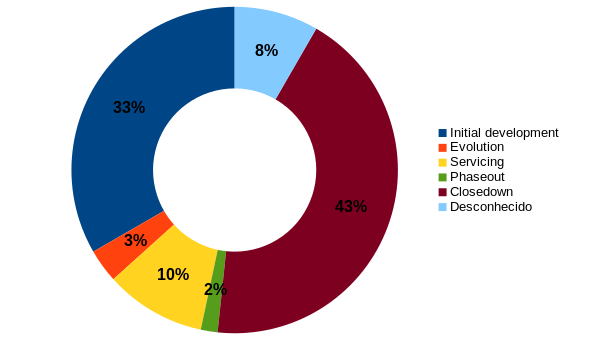
\includegraphics[scale=0.55]{imagens/life-cycle-pie.png}
  \end{minipage}
  \begin{minipage}{0.5\textwidth}
    \centering
    \begin{tabular}{l c}
  \hline
  {\bf Estágio} & {\bf Projetos} \\
  \hline
    Initial development & 20 \\
    Evolution & 2 \\
    Servicing & 6 \\
    Phaseout & 3 \\
    Closedown & 24 \\
    Desconhecido & 5 \\
  \hline
\end{tabular}

  \end{minipage}
  \caption{Número total de projetos identificados em cada estágio de evolução.}
  \label{life-cycle}
\end{figure}

Entre os projetos em fase de evolução ou serviço estão aqueles com maior número
de lançamentos. Os projetos em estágio {\it Initial development} possuem
características de ser software acadêmico do tipo Software Incidental ({\it
Incidental software}) e ter sido feito puramente para apoiar e facilitar
pesquisas, enquanto os projetos em estágio {\it Evolution} e {\it Servicing}
possi características de ser software acadêmico do tipo Prática de software
paralela ({\it A parallel software practice}) feito com objetivo de ser
utilizado por outros pesquisadores ou Um subcampo de software ({\it A Software
Sub-field}) onde o próprio software é considerado uma contribuição primária
para a Ciência.

%\begin{figure}[h]
%  \begin{minipage}{0.32\textwidth}
%    \centering
%    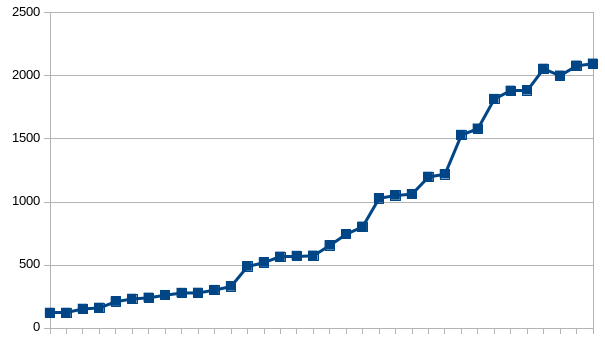
\includegraphics[scale=0.32]{imagens/evolution-s6.png}
%    \texttt{s6}
%  \end{minipage}
%  \begin{minipage}{0.32\textwidth}
%    \centering
%    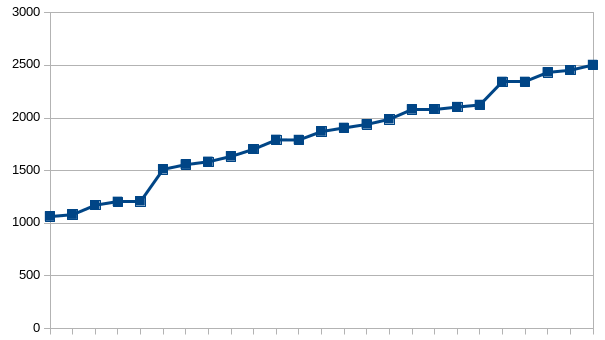
\includegraphics[scale=0.32]{imagens/evolution-s18.png}
%    \texttt{s18}
%  \end{minipage}
%  \begin{minipage}{0.32\textwidth}
%    \centering
%    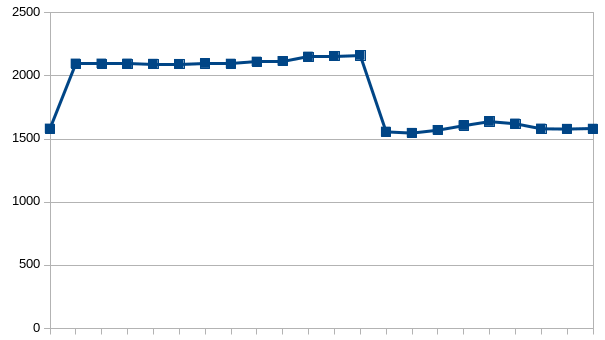
\includegraphics[scale=0.32]{imagens/evolution-s26.png}
%    \texttt{s26}
%  \end{minipage}
%
%\vspace{3mm}
%
%  \begin{minipage}{0.32\textwidth}
%    \centering
%    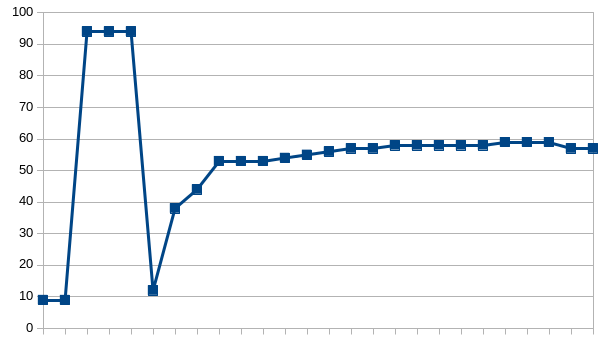
\includegraphics[scale=0.32]{imagens/evolution-s28.png}
%    \texttt{s28}
%  \end{minipage}
%  \begin{minipage}{0.32\textwidth}
%    \centering
%    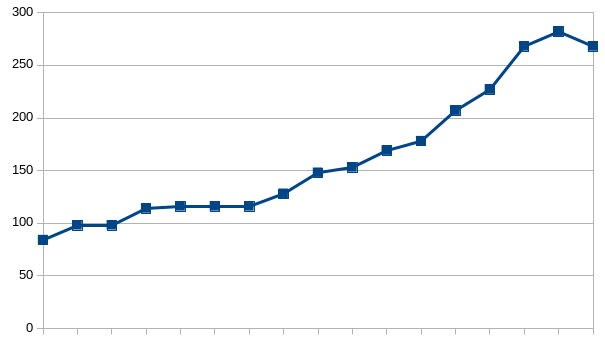
\includegraphics[scale=0.32]{imagens/evolution-s51.png}
%    \texttt{s51}
%  \end{minipage}
%  \begin{minipage}{0.32\textwidth}
%    \centering
%    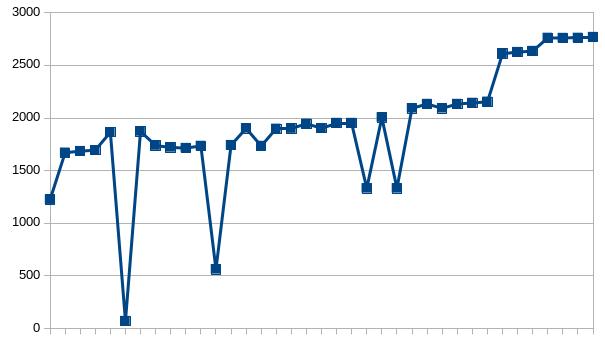
\includegraphics[scale=0.32]{imagens/evolution-s58.png}
%    \texttt{s58}
%  \end{minipage}
%  \caption{Variação no número de módulos dos projetos em fase de {\it Servicing}.}
%  \label{evolution-graph}
%\end{figure}

% }}}

\section{Ameaças à validade} % {{{

Toda a análise e interpretação dos resultados tomou como base apenas os dados
coletados do site, publicações, e repositórios dos projetos de software
acadêmico de análise estática, o fato de não incluirmos coleta de dados a
partir das pessoas envolvidas nos projetos pode enfraquecer alguma conclusão no
sentido de que alguns projetos podem ter definições explícitas por parte dos
seus desenvolvedores mas que não se refletem ainda nos documentos dos projetos,
apesar disso o nosso estudo tem um caráter exploratório, com interesse especial em
uma figura geral do domínio de análise estática e não necessariamente trazer
evidências sobre os projetos inidivualmente.

% }}}

\section{Conclusões} \label{estudo3:conclusoes} % {{{

Este estudo coletou informações de \ReleasesCount \ lançamentos em relação a
\ProjectsWithReleasesCount \ projetos de software acadêmico de análise
estática. Analisou e extraiu o número de módulos do código fonte de
\ReleasesMetricsCount \ versões distintas destes projetos.

A partir destes dados caracterizou cada um dos \SoftwareCount \ projetos
estudados em relação ao estágio de evolução do ciclo de vida do software e
identificou que a grande maioria encontra-se em estado inicial de
desenvolvimento ou encerrados (76\%).

Apenas 2 projetos encontram-se em evoluçao atualmente, com variação no número
de módulos nos últimos lançamentos recentes superior a 10\%. E 6 projetos em
fase de serviço, indicando que são projetos estáveis com atualizações
constantes mas com pouca variação na base de código do projeto.

Os dados, interpretações e conclusões deste estudo e dos dois estudos
anteriores apresentados nos Capítulos \ref{estudo1} e \ref{estudo2} serão
analisados em conjunto e discutidos no capítulo seguinte sob uma mesma
perspectiva em relação à sustentabilidade técnica do ecossistema de software
acadêmico de análise estática, no recorte de projetos selecionados nas
conferências de Engenharia de Software ASE e SCAM, entre menções encontradas
nas bases ACM e IEEE, e com análise ao nível de código fonte dos projetos
escritos em C, C++ e Java.

% }}}


%------------------------------------------%

\xchapter{Conclusões}{}
\label{conclusoes}

%Mas independente de como seja calculado o impacto científico de uma determinada
%pesquisa o impacto causado se reverte potencialmente em mais recursos que
%poderão ser reinvestidos no próprio ecossistema onde o software está inserido.


O desenvolvimento de software acadêmico, de forma sustentável,
abre portas para elevar a qualidade geral do software e
da pesquisa científica, promovendo a reproducibilidade e
proporcionando um ambiente de compartilhamento e colaboração 
em oposição ao tradicional modelo de competição que permeia
o sistema de reputação e crédito científico.
%
Na área de engenharia de software, 
especialmente no domínio de análise estática,
com tradição no desenvolvimento de ferramentas para apoiar pesquisas
em diferentes áreas da ciência da computação,
a preocupação com a sustentabilidade técnica em software acadêmico
não pode ser desconsiderada. 

Esta pesquisa de mestrado caracterizou
projetos de software acadêmico de análise estática,
publicados até 2015 em artigos científicos das conferências ASE e SCAM,
em relação a sua sustentabilidade técnica, definida
em termos de publicização, reconhecimento e ciclo de vida.
%
O estudo sobre a publicização
%de software acadêmico de análise estática 
identificou 60 projetos de software acadêmico de análise estática
publicados originalmente nas conferências ASE e SCAM.
A caracterização da publicização desses projetos considerou
disponibilidade para download, acesso ao código fonte, forma de distribuição e licença.
Apenas 3\% dos 1873 artigos publicados nas conferências ASE e SCAM 
publicizaram software acadêmico de análise estática de forma adequada,
com indicação de URL para download.
%
O estudo sobre reconhecimento 
inspecionou \SearchUniqueCount \ artigos encontrados nas bases ACM
e IEEE através de busca avançada, 
usando características de \SoftwareCount \ projetos 
de software acadêmico de análise estática. 
A inspeção identificou  \ScreeningCount \ menções 
dos tipos \texttt{Cita}, \texttt{Usa} ou \texttt{Contribui}.
Houve um crescimento de 38\% ao ano no número de menções ao software acadêmico, 
e apenas 10\% do total de menções realizam contribuição de código fonte dos
projetos.
%
O estudo sobre ciclo de vida
caracterizou o estágio de evolução de software acadêmico de análise estática
com código fonte disponível,
considerando o número de lançamentos e de módulos no código fonte,
e revelou que a maior parte dos projetos encontra-se 
em estágio inicial de desenvolvimento ou encerrado.

Ao sintetizar os resultados (capítulo~\ref{discussao}) para responder a questão
geral de pesquisa ({\it \QuestaoGeralUm}) percebemos que a DCD é útil para
explicar a sustentabilidade técnica de um domínio de aplicação em níveis
distintos de profundidade, através da seguintes características:

\begin{description}
  \item [C1] Existência de muitos projetos com poucos usuários;
  \item [C2] Cada projeto tendo ciclos de vida curtos que se encerram junto ao financiamento inicial;
  \item [C3] Comunidades de usuários desconectadas e paralelas;
  \item [C4] Incompatibilidades entre os projetos de maneira persistente e imutável;
  \item [C5] Tentativas constantes e aparentemente não coordenadas de ``reiniciar'' tudo ({\it re-boots}).
\end{description}

Em nosso estudo utilizamos as características {\bf C1} e {\bf C2} da DCD para
explicar a sustentabilidade técnica dos projetos do ecossistema de análise
estática e percebemos que neste domínio há muitos projetos de software
acadêmico indisponíveis ou encerrados (78\%), com pouco reconhecimento e com
poucos usuários, com ciclos de vida curtos ou em estágio inicial de
desenvolvimento, revelando um ecossistema em que há pouca colaboração e
indícios de graves problemas de sustentabilidade.

%... a característica 
%(Existência de muitos projetos com poucos usuários) foi ... neste domínio; a
%característica 
%encerram junto ao financiamento inicial) foi parcialmente demonstrada onde
%projetos possuem ciclos de vida curtos, mas não coletados dados para realizar
%estudo sobre o financiamento dos projetos; as características {\bf C3}, {\bf
%C4} e {\bf C5} não foram avaliadas.

%sendo
%desordem caótica disfuncional ({\it ``dysfunctional chaotic churn''}),
%caracterizado por \cite{howison2015understanding}:

%A caracterização da sustentabilidade técnica de 
%software acadêmico de análise estática, no contexto de 
%60 projetos de análise estática estudados, mostrou que 
%há muitos projetos de software acadêmico indisponíveis ou encerrados (78\%), 
%com pouco reconhecimento, com poucos usuários, 
%e ciclos de vida curtos ou em estágio inicial de desenvolvimento,
%revelando um ecossistema em que há pouca colaboração
%e indícios de sintomas de desordem caótica disfuncional.

\section{Contribuições}

A caracterização da sustentabilidade técnica de software acadêmico de análise estática
publicado nas conferências de Engenharia de Software ASE e SCAM 
mapeou os projetos de software disponíveis e o grau de evolução que
se encontram no ciclo de vida.

Este mapeamento abre caminho para a compreensão de problemas relacionados a 
sustentabilidade de software acadêmico de análise estática 
e posterior definição de estratégias para
solucionar e melhorar o campo, tanto em termos práticos quanto teóricos.

O conhecimento a respeito dos projetos de software acadêmico de análise estática
existentes serve aos interessados em utilizar tais projetos em novas pesquisas,
seja como objeto de estudo, como apoio metodológico, ou ainda, como base para
iniciar novos desenvolvimentos.

%especialmente entre os projetos em estágio inicial, que apresentam em alguns casos
%indícios de estarem abandonados mas o código fonte deles possui grande potencial
%de ser útil e reduzir o caminho tomado em novas pesquisas.

Esta pesquisa contribui ainda com uma auto-reflexão sobre o campo de análise
estática e seus projetos de software acadêmico, especialmente em relação ao
esforço e recursos investidos no desenvolvimento de software neste domínio de
aplicação sendo consumidos de maneira ineficiente.

%, para que
%a partir daí, como exercício resolver estes problemas e reduzir duplicação de esforço e retrabalho.

No campo teórico, contribui para uma melhor compreensão do que vem a ser
sustentabilidade de software, um tema que ainda carece de definição clara,
especialmente sustentabilidade de software acadêmico de análise estática.

%além de contribui para
%uma definição teórica e prática sobre ecossistema de software acadêmico de análise estática.

Por fim, contribui alertando para os prejuízos que a indisponibilidade de
código destes projetos causam para a Ciência, uma vez que acesso ao código é
parte fundamental para validar ou refutar conclusões de pesquisas através da
reprodução e replicação.

%ou reproduir estudos do passado é uma excelente forma, tanto de validar ou refutar conclusões,
%quanto de contribuir evoluindo as pesquisa e os dados, além de ser tb uma oportunidade
%de evoluir os próprios códigos.

%6 ...  A caracterização ... contribuir para a sustentabilidade do software acadêmico
%de análise estática.

\section{Limitações}

%Escopo limitado.

O escopo do estudo limitou-se a selecionar software acadêmico em apenas um
domínio de aplicação, análise estática, e em apenas duas conferências de
Engenharia de Software, ASE e SCAM, e ainda, usando como data limite o ano de
2015. A busca por menções aos projetos também foi limitado a apenas duas
bibliotecas de indexação de publicações, ACM e IEEE.

%apenas projetos publicados com URL e indicados que estão disponíveis para download
%não levar em consideração o fator de impacto das conferências onde os artigos foram publicados

Além da limitação de escopo, este estudo realizou também uma série de
procedimentos manuais, a revisao de literatura para seleção de software
acadêmico foi realizada manualmente, a execução da busca nas bases ACM e IEEE
foi feita em atividades manuais.

%Procedimentos manuais.
%extração de informações de cada projeto também totalmente manual, incluindo as buscas nas bases ACM e IEEE
%coleta de dados ...

\section{Trabalhos futuros}

% Sobre escopo

O trabalho mais imediato para extender esta pesquisa seria atualizar a revisão
de literatura inicial para extender o período de seleção de software acadêmico
de análise estática incluindo os anos de 2016 e 2017, uma vez que esta
dissertação limitou a seleção ao ano de 2015.

Outro trabalho importante é ampliar o escopo do estudo incluindo mais
conferências visando aumentar o realismo sobre o domínio estudado,
especialmente conferências tradicionais de Engenharia de Software, como por
exemplo, a conferência ICSE (International Conference on Software
Engineering)\footnote{\url{http://www.icse-conferences.org}} por ser uma das
mais tradicionais e importantes conferências da área de Engenharia de Software.
Consideramos também ser importante incluir o congresso CBSOFT (Congresso
Brasileiro de Software: Teoria e Prática)\footnote{\url{http://www.cbsoft.org}}
por ser uma importante conferência no contexto Brasileiro de Engenharia de
Software, com longo histórico, e trilhas de publicação de ferramentas.

% Sobre procedimentos manuais
Usar técnicas de ... para identificar automaticamente menções e seus tipos ...
VER com Rodrigo.

% Sobre extensões: novas questões

Outro ponto em relação a conferências é coletar o fator de impacto da
conferência e utilizar esta informação na análise dos dados e discussão, é
possível que conferências com maior fator de impacto apresentem projetos com
maior reconhecimento e com características de publicização mais adequadas.

Além de ampliar o escopo de forma horizontal incluindo novas conferências, é
interessante também aumentar a qualidade da caracterização do software
incluindo novas dimensões de caracterização, especialmente dimensões na visão
de usuário, como por exemplo, documentação, facilidade de instalaçao, execução,
existência de manuais, avaliar o nível de descrição e apresentação do software
no site ou repositório, ou mesmo incluir aspectos de Engenharia de Software,
como por exemplo, testes, resolução de {\it issues}, métricas de qualidade como
por exemplo complexidade estrutural, número de contribuidores, número de
commits e uso de controle de versão.

%O autor do software provê informações sobre como citar o software apropriadmente? \cite{allen2017engineering}

Uma outra forma de enriquecer a caracterização de cada software é usar
caracterizações já realizadas em outros trabalhos científicos, muitos estudos
avaliam e comparam ferramentas de análise estática entre sí, os artigos
encontrados na seleção de software acadêmico são os primeiros candidatos a
serem utilizados como fonte de coleta de dados sobre cada software.

%apenas caracterizaçõas mas também avaliações, ou seja, entrar no conteúdo dos
%artigos encontrados sobre cada software, e usar as informações já
%caracterizadas para compor uma caracterização mais rica do conjunto de
%ferramentas.

%incluir outras bases na primeira revisão (estruturada) realizada para
%ver se outras ferramentas importantes não ficaram de for.

Outra possibilidade de trabalho futuro é revisar artigos publicados em jornais
com foco específico em publicação de software em busca mais projetos de
software acadêmico de análise estática, entre estes jornais podemos citar, por
exemplo, o JORS (Journal of Open Research
Software)\footnote{\url{https://openresearchsoftware.metajnl.com/articles/10.5334/jors.bt}},
JOSS (Journal of Open Source Software)\footnote{\url{http://joss.theoj.org}} \cite{smith2017journal} e
o SoftwareX\footnote{\url{https://www.journals.elsevier.com/softwarex}} da
Elsevier. 

%Incluir e avaliar ferramentas publicadas e apresentadas no evento de
%ferramentas da UFBA.
%
%Medir a usabilidade do software acadêmico de análise estática e como podem ser
%mais úteis ao desenvolvedor de modo geral, especialmente para o cientista
%desenvolvedor de software.
%
%Investigar o impacto da sustentabilidade técnica do software acadêmico na
%reprodutibilidade dos estudos que fazem uso do software como apoio metodológico
%(coleta ou análise).


%------------------------------------------%

\backmatter
\bibliography{bibliografia}

\appendix
\xchapter{Reproducibilidade do estudo}
{Este capítulo apresenta ....}
\label{reproducibilidade-do-estudo}

% TODO
% documentar instalação das dependencias do script para filtro
% documentar a instaação do sloccount
% descrever o formato YAML utilizado para caracterização dos projetos

%produz um resultado indicando todas as linguagens e
%quanto do código total é escrito em cada uma delas.

Apresentar e detalhar os arquivos scam-links.md e ase-link.md (citado no estudo1:preparacao).

Os artigos analisados na revisão estruturada estão todos documentados arquivo
{\it
dataset/dataset.ods}\footnote{\url{http://github.com/joenio/dissertacao-ufba-2016/blob/master/dataset/dataset.ods}},
uma planilha no formato aberto {\it Open Document Format for Office
Applications}\footnote{\url{http://www.oasis-open.org/committees/office}}.

Nesta planilha está documentada cada etapa da revisão estruturada, indicando em
cada artigo analisado qual o estado do mesmo, se foi ou não incluído na
execução da atividade.  Nesta planilha é possível encontrar também o nome de
cada ferramenta e uma caracterização completa.

O script utilizado na segunda atividade da revisão estruturada -- {\it (2)
Filtro} -- também está neste mesmo repositório no arquivo {\it
dataset/revisao-estruturada/filter}\footnote{\url{http://github.com/joenio/dissertacao-ufba-2016/blob/master/revisao-estruturada/filter}}
escrito em linguagem Perl especialmente para este estudo.

A maior parte das atividades de pesquisa, reuniões de orientação e comunicação
realizadas neste estudo estão também documentadas em {\it issues} neste
repositório e na wiki do grupo de pesquisa aSide.

\begin{itemize}
  \item \url{http://wiki.dcc.ufba.br/Aside/Orientacao2014JoenioCosta}
  \item \url{https://github.com/joenio/dissertacao-ufba-2016/issues}
\end{itemize}


%------------------------------------------%

\end{document}

% vim: filetype=tex
